%%%%%%%%%%%%%%%%%%%%%%%%%%%%%%%%%%%%%%%%%%%%%%%%%%%%%%%%%%%%%%%
%% OXFORD THESIS TEMPLATE

% Use this template to produce a standard thesis that meets the Oxford University requirements for DPhil submission
%
% Originally by Keith A. Gillow (gillow@maths.ox.ac.uk), 1997
% Modified by Sam Evans (sam@samuelevansresearch.org), 2007
% Modified by John McManigle (mcmanigle@gmail.com), 2015

% I've (John) tried to comment this file extensively, so read through it to see how to use the various options.  Remember
% that in LaTeX, any line starting with a % is NOT executed.  Several places below, you have a choice of which line to use
% out of multiple options (eg draft vs final, for PDF vs for binding, etc.)  When you pick one, add a % to the beginning of
% the lines you don't want.


%%%%% CHOOSE PAGE LAYOUT
% The most common choices should be below.  You can also do other things, like replacing "a4paper" with "letterpaper", etc.

% This one will format for two-sided binding (ie left and right pages have mirror margins; blank pages inserted where needed):
\documentclass[hidelinks, a4paper,twoside]{ociamthesis}
% This one will format for one-sided binding (ie left margin > right margin; no extra blank pages):
%\documentclass[a4paper]{ociamthesis}
% This one will format for PDF output (ie equal margins, no extra blank pages):
%\documentclass[a4paper,nobind]{ociamthesis} 

\usepackage{graphbox}

\usepackage{svg}
\usepackage{tabularx}
\renewcommand\tabularxcolumn[1]{m{#1}}% for vertical centering text in X column

\usepackage{tikz} 

\usepackage{listings}

%%%%% SELECT YOUR DRAFT OPTIONS
% Three options going on here; use in any combination.  But remember to turn the first two off before
% generating a PDF to send to the printer!

% This adds a "DRAFT" footer to every normal page.  (The first page of each chapter is not a "normal" page.)
\fancyfoot[C]{\emph{DRAFT Printed on \today}}  

% This highlights (in blue) corrections marked with (for words) \mccorrect{blah} or (for whole
% paragraphs) \begin{mccorrection} . . . \end{mccorrection}.  This can be useful for sending a PDF of
% your corrected thesis to your examiners for review.  Turn it off, and the blue disappears.
\correctionstrue


%%%%% BIBLIOGRAPHY SETUP
% Note that your bibliography will require some tweaking depending on your department, preferred format, etc.
% The options included below are just very basic "sciencey" and "humanitiesey" options to get started.
% If you've not used LaTeX before, I recommend reading a little about biblatex/biber and getting started with it.
% If you're already a LaTeX pro and are used to natbib or something, modify as necessary.
% Either way, you'll have to choose and configure an appropriate bibliography format...

% The science-type option: numerical in-text citation with references in order of appearance.
\usepackage[style=numeric-comp, sorting=none, backend=biber, doi=false, isbn=false]{biblatex}
\newcommand*{\bibtitle}{References}

% The humanities-type option: author-year in-text citation with an alphabetical works cited.
%\usepackage[style=authoryear, sorting=nyt, backend=biber, maxcitenames=2, useprefix, doi=false, isbn=false]{biblatex}
%\newcommand*{\bibtitle}{Works Cited}

% This makes the bibliography left-aligned (not 'justified') and slightly smaller font.
\renewcommand*{\bibfont}{\raggedright\small}

% Change this to the name of your .bib file (usually exported from a citation manager like Zotero or EndNote).
\addbibresource{references.bib}


% Uncomment this if you want equation numbers per section (2.3.12), instead of per chapter (2.18):
%\numberwithin{equation}{subsection}



%%%%% THESIS / TITLE PAGE INFORMATION
% Everybody needs to complete the following:
\title{Design and modular self-assembly of nanostructures}
\author{Joakim Bohlin}
\college{Balliol College}

% Master's candidates who require the alternate title page (with candidate number and word count)
% must also un-comment and complete the following three lines:
%\masterssubmissiontrue
%\candidateno{933516}
%\wordcount{28,815}

% Uncomment the following line if your degree also includes exams (eg most masters):
%\renewcommand{\submittedtext}{Submitted in partial completion of the}
% Your full degree name.  (But remember that DPhils aren't "in" anything.  They're just DPhils.)
\degree{Doctor of Philosophy}
% Term and year of submission, or date if your board requires (eg most masters)
\degreedate{Michaelmas 2021}


%%%%% YOUR OWN PERSONAL MACROS
% This is a good place to dump your own LaTeX macros as they come up.

% To make text superscripts shortcuts
	\renewcommand{\th}{\textsuperscript{th}} % ex: I won 4\th place
	\newcommand{\nd}{\textsuperscript{nd}}
	\renewcommand{\st}{\textsuperscript{st}}
	\newcommand{\rd}{\textsuperscript{rd}}



%%%%% THE ACTUAL DOCUMENT STARTS HERE
\begin{document}

%%%%% CHOOSE YOUR LINE SPACING HERE
% This is the official option.  Use it for your submission copy and library copy:
\setlength{\textbaselineskip}{22pt plus2pt}
% This is closer spacing (about 1.5-spaced) that you might prefer for your personal copies:
%\setlength{\textbaselineskip}{18pt plus2pt minus1pt}

% You can set the spacing here for the roman-numbered pages (acknowledgements, table of contents, etc.)
\setlength{\frontmatterbaselineskip}{17pt plus1pt minus1pt}

% Leave this line alone; it gets things started for the real document.
\setlength{\baselineskip}{\textbaselineskip}


%%%%% CHOOSE YOUR SECTION NUMBERING DEPTH HERE
% You have two choices.  First, how far down are sections numbered?  (Below that, they're named but
% don't get numbers.)  Second, what level of section appears in the table of contents?  These don't have
% to match: you can have numbered sections that don't show up in the ToC, or unnumbered sections that
% do.  Throughout, 0 = chapter; 1 = section; 2 = subsection; 3 = subsubsection, 4 = paragraph...

% The level that gets a number:
\setcounter{secnumdepth}{2}
% The level that shows up in the ToC:
\setcounter{tocdepth}{2}


%%%%% ABSTRACT SEPARATE
% This is used to create the separate, one-page abstract that you are required to hand into the Exam
% Schools.  You can comment it out to generate a PDF for printing or whatnot.
\begin{abstractseparate}
	Your abstract text goes here.  Check your departmental regulations, but generally this should be less than 300 words.  See the beginning of Chapter~\ref{ch:2-litreview} for more.

Lorem ipsum dolor sit amet, consectetur adipiscing elit. Pellentesque sit amet nibh volutpat, scelerisque nibh a, vehicula neque. Integer placerat nulla massa, et vestibulum velit dignissim id. Ut eget nisi elementum, consectetur nibh in, condimentum velit. Quisque sodales dui ut tempus mattis. Duis malesuada arcu at ligula egestas egestas. Phasellus interdum odio at sapien fringilla scelerisque. Mauris sagittis eleifend sapien, sit amet laoreet felis mollis quis. Pellentesque dui ante, finibus eget blandit sit amet, tincidunt eu neque. Vivamus rutrum dapibus ligula, ut imperdiet lectus tincidunt ac. Pellentesque ac lorem sed diam egestas lobortis.

Suspendisse leo purus, efficitur mattis urna a, maximus molestie nisl. Aenean porta semper tortor a vestibulum. Suspendisse viverra facilisis lorem, non pretium erat lacinia a. Vestibulum tempus, quam vitae placerat porta, magna risus euismod purus, in viverra lorem dui at metus. Sed ac sollicitudin nunc. In maximus ipsum nunc, placerat maximus tortor gravida varius. Suspendisse pretium, lorem at porttitor rhoncus, nulla urna condimentum tortor, sed suscipit nisi metus ac risus.

Aenean sit amet enim quis lorem tristique commodo vitae ut lorem. Duis vel tincidunt lacus. Sed massa velit, lacinia sed posuere vitae, malesuada vel ante. Praesent a rhoncus leo. Etiam sed rutrum enim. Pellentesque lobortis elementum augue, at suscipit justo malesuada at. Lorem ipsum dolor sit amet, consectetur adipiscing elit. Praesent rhoncus convallis ex. Etiam commodo nunc ex, non consequat diam consectetur ut. Pellentesque vitae est nec enim interdum dapibus. Donec dapibus purus ipsum, eget tincidunt ex gravida eget. Donec luctus nisi eu fringilla mollis. Donec eget lobortis diam.

Suspendisse finibus placerat dolor. Etiam ornare elementum ex ut vehicula. Donec accumsan mattis erat. Quisque cursus fringilla diam, eget placerat neque bibendum eu. Ut faucibus dui vitae dolor porta, at elementum ipsum semper. Sed ultrices dui non arcu pellentesque placerat. Etiam posuere malesuada turpis, nec malesuada tellus malesuada. % Create an abstract.tex file in the 'text' folder for your abstract.
\end{abstractseparate}


% JEM: Pages are roman numbered from here, though page numbers are invisible until ToC.  This is in
% keeping with most typesetting conventions.
\begin{romanpages}

% Title page is created here
\maketitle

%%%%% DEDICATION -- If you'd like one, un-comment the following.
%\begin{dedication}
%This thesis is dedicated to\\
%someone\\
%for some special reason\\
%\end{dedication}

%%%%% ACKNOWLEDGEMENTS -- Nothing to do here except comment out if you don't want it.
\begin{acknowledgements}
 	\subsection*{Personal}

This is where you thank your advisor, colleagues, and family and friends.

Lorem ipsum dolor sit amet, consectetur adipiscing elit. Vestibulum feugiat et est at accumsan. Praesent sed elit mattis, congue mi sed, porta ipsum. In non ullamcorper lacus. Quisque volutpat tempus ligula ac ultricies. Nam sed erat feugiat, elementum dolor sed, elementum neque. Aliquam eu iaculis est, a sollicitudin augue. Cras id lorem vel purus posuere tempor. Proin tincidunt, sapien non dictum aliquam, ex odio ornare mauris, ultrices viverra nisi magna in lacus. Fusce aliquet molestie massa, ut fringilla purus rutrum consectetur. Nam non nunc tincidunt, rutrum dui sit amet, ornare nunc. Donec cursus tortor vel odio molestie dignissim. Vivamus id mi erat. Duis porttitor diam tempor rutrum porttitor. Lorem ipsum dolor sit amet, consectetur adipiscing elit. Sed condimentum venenatis consectetur. Lorem ipsum dolor sit amet, consectetur adipiscing elit.

Aenean sit amet lectus nec tellus viverra ultrices vitae commodo nunc. Mauris at maximus arcu. Aliquam varius congue orci et ultrices. In non ipsum vel est scelerisque efficitur in at augue. Nullam rhoncus orci velit. Duis ultricies accumsan feugiat. Etiam consectetur ornare velit et eleifend.

Suspendisse sed enim lacinia, pharetra neque ac, ultricies urna. Phasellus sit amet cursus purus. Quisque non odio libero. Etiam iaculis odio a ex volutpat, eget pulvinar augue mollis. Mauris nibh lorem, mollis quis semper quis, consequat nec metus. Etiam dolor mi, cursus a ipsum aliquam, eleifend venenatis ipsum. Maecenas tempus, nibh eget scelerisque feugiat, leo nibh lobortis diam, id laoreet purus dolor eu mauris. Pellentesque habitant morbi tristique senectus et netus et malesuada fames ac turpis egestas. Nulla eget tortor eu arcu sagittis euismod fermentum id neque. In sit amet justo ligula. Donec rutrum ex a aliquet egestas.

\subsection*{Institutional}

This project has received funding from the European Union’s Horizon 2020 research and innovation programme under the Marie Skłodowska-Curie grant agreement No 765703

If you want to separate out your thanks for funding and institutional support, I don't think there's any rule against it.  Of course, you could also just remove the subsections and do one big traditional acknowledgement section.

Lorem ipsum dolor sit amet, consectetur adipiscing elit. Ut luctus tempor ex at pretium. Sed varius, mauris at dapibus lobortis, elit purus tempor neque, facilisis sollicitudin felis nunc a urna. Morbi mattis ante non augue blandit pulvinar. Quisque nec euismod mauris. Nulla et tellus eu nibh auctor malesuada quis imperdiet quam. Sed eget tincidunt velit. Cras molestie sem ipsum, at faucibus quam mattis vel. Quisque vel placerat orci, id tempor urna. Vivamus mollis, neque in aliquam consequat, dui sem volutpat lorem, sit amet tempor ipsum felis eget ante. Integer lacinia nulla vitae felis vulputate, at tincidunt ligula maximus. Aenean venenatis dolor ante, euismod ultrices nibh mollis ac. Ut malesuada aliquam urna, ac interdum magna malesuada posuere.
\end{acknowledgements}

%%%%% ABSTRACT -- Nothing to do here except comment out if you don't want it.
\begin{abstract}
	Your abstract text goes here.  Check your departmental regulations, but generally this should be less than 300 words.  See the beginning of Chapter~\ref{ch:2-litreview} for more.

Lorem ipsum dolor sit amet, consectetur adipiscing elit. Pellentesque sit amet nibh volutpat, scelerisque nibh a, vehicula neque. Integer placerat nulla massa, et vestibulum velit dignissim id. Ut eget nisi elementum, consectetur nibh in, condimentum velit. Quisque sodales dui ut tempus mattis. Duis malesuada arcu at ligula egestas egestas. Phasellus interdum odio at sapien fringilla scelerisque. Mauris sagittis eleifend sapien, sit amet laoreet felis mollis quis. Pellentesque dui ante, finibus eget blandit sit amet, tincidunt eu neque. Vivamus rutrum dapibus ligula, ut imperdiet lectus tincidunt ac. Pellentesque ac lorem sed diam egestas lobortis.

Suspendisse leo purus, efficitur mattis urna a, maximus molestie nisl. Aenean porta semper tortor a vestibulum. Suspendisse viverra facilisis lorem, non pretium erat lacinia a. Vestibulum tempus, quam vitae placerat porta, magna risus euismod purus, in viverra lorem dui at metus. Sed ac sollicitudin nunc. In maximus ipsum nunc, placerat maximus tortor gravida varius. Suspendisse pretium, lorem at porttitor rhoncus, nulla urna condimentum tortor, sed suscipit nisi metus ac risus.

Aenean sit amet enim quis lorem tristique commodo vitae ut lorem. Duis vel tincidunt lacus. Sed massa velit, lacinia sed posuere vitae, malesuada vel ante. Praesent a rhoncus leo. Etiam sed rutrum enim. Pellentesque lobortis elementum augue, at suscipit justo malesuada at. Lorem ipsum dolor sit amet, consectetur adipiscing elit. Praesent rhoncus convallis ex. Etiam commodo nunc ex, non consequat diam consectetur ut. Pellentesque vitae est nec enim interdum dapibus. Donec dapibus purus ipsum, eget tincidunt ex gravida eget. Donec luctus nisi eu fringilla mollis. Donec eget lobortis diam.

Suspendisse finibus placerat dolor. Etiam ornare elementum ex ut vehicula. Donec accumsan mattis erat. Quisque cursus fringilla diam, eget placerat neque bibendum eu. Ut faucibus dui vitae dolor porta, at elementum ipsum semper. Sed ultrices dui non arcu pellentesque placerat. Etiam posuere malesuada turpis, nec malesuada tellus malesuada.
\end{abstract}

%%%%% MINI TABLES
% This lays the groundwork for per-chapter, mini tables of contents.  Comment the following line
% (and remove \minitoc from the chapter files) if you don't want this.  Un-comment either of the
% next two lines if you want a per-chapter list of figures or tables.
\dominitoc % include a mini table of contents
%\dominilof  % include a mini list of figures
%\dominilot  % include a mini list of tables

% This aligns the bottom of the text of each page.  It generally makes things look better.
\flushbottom

% This is where the whole-document ToC appears:
\tableofcontents

\listoffigures
	\mtcaddchapter
% \mtcaddchapter is needed when adding a non-chapter (but chapter-like) entity to avoid confusing minitoc

% Uncomment to generate a list of tables:
\listoftables
	\mtcaddchapter

%%%%% LIST OF ABBREVIATIONS
% This example includes a list of abbreviations.  Look at text/abbreviations.tex to see how that file is
% formatted.  The template can handle any kind of list though, so this might be a good place for a
% glossary, etc.
% First parameter can be changed eg to "Glossary" or something.
% Second parameter is the max length of bold terms.
\begin{mclistof}{Glossary}{3.2cm}

\item[2D, 3D] Two- or three-dimensional, referring in this thesis to spatial dimensions of a self-assembled structure.
\item[AIT] Algorithmic Information Theory
\item[DNA] Deoxyribonucleic acid.
\item[RNA] Ribonucleic acid.
\item[PDB] The Protein Data Bank (\url{https://www.wwpdb.org/}). Used in this thesis to refer to the file format used to save atomic structures.
\item[Polycube] A 3D shape consisting of multiple cubes connected by their sides.
\item[Polyomino] A 2D shape consisting of multiple squares connected by their edges.
\item[SAT] Boolean satisfiability.
\item[Species] Used in this thesis to denote a type of cube allowed by the polycube rule.
\item[TEM] Transmission Electron Microscopy 

\end{mclistof} 


% The Roman pages, like the Roman Empire, must come to its inevitable close.
\end{romanpages}

%Instead, let's talk a little about a few of the features and packages lumped into this template situation.  The \verb|savequote| environment at the beginning of chapters can add some wittiness to your thesis.  If you don't like the quotes, just remove that block.

%For when it comes time to do corrections, there are two useful commands here.  First, the \verb|mccorrect| command allows you to highlight a short correction \mccorrect{like this one}.  When the thesis is typeset normally, the correction will just appear as part of the text.  However, when you declare \verb|\correctionstrue| in the main \verb|Oxford_Thesis.tex| file, that correction will be highlighted in blue.  That might be useful for submitting a post-viva, corrected copy to your examiners so they can quickly verify you've completed the task.

%\begin{mccorrection}
%For larger chunks, like this paragraph or indeed entire figures, you can use the \verb|mccorrection| environment.  This environment highlights paragraph-sized and larger blocks with the same blue colour.
%\end{mccorrection}

%Read through the \verb|Oxford_Thesis.tex| file to see the various options for one- and two-sided printing, including or excluding the separate abstract page, and turning corrections and draft footer on or off, and the separate option to centre your text on the page (for PDF submission) or offset it (for binding).  There is also a separate option for master's degree submissions, which changes identifying information to candidate number and includes a word count.  (Unfortunately, \LaTeX has a hard time doing word counts automatically, so you'll have to enter the count manually if you require this.)


%%%%% CHAPTERS
% Add or remove any chapters you'd like here, by file name (excluding '.tex'):
\flushbottom
%\begin{savequote}[8cm]
%Far out in the uncharted backwaters of the unfashionable end of the western spiral arm of the Galaxy lies a small unregarded yellow sun. Orbiting this at a distance of roughly ninety-two million miles is an utterly insignificant little blue green planet whose ape-descended life forms are so amazingly primitive that they still think digital watches are a pretty neat idea.
%  \qauthor{--- D. Adams, The Hitchhiker's Guide to the Galaxy}
%\end{savequote}

\chapter{Introduction}\label{ch:1-intro}

\minitoc

How do you design and assemble something on the nanoscale? When working with everyday objects on the macroscale, it is easy to pick the building blocks you want and attach them where you want them to be. However, for nanoscale objects it is difficult to have that level of top-down control. Instead, more success has been had by imitating nature and letting the building blocks assemble themselves. After millions of years of evolution, nature has the advantage. This thesis will cover novel methods and tools to design such self-assembling nanostructures.

\section{Background}
I am pursuing my graduate studies in Condensed Matter Physics as an Early-Stage Researcher, part of a Marie Skłodowska-Curie Innovative Training Network called \emph{DNA-Robotics}\footnote{\url{https://dna-robotics.eu/}, grant agreement number 765703}. The network consists of the leading European DNA nanotechnology research groups and was formed with the goal of creating a unified framework for integrated biomolecular robotics\cite{dnaroboticsResearch}.

My position, in particular, is assigned to develop standardised techniques for the design and self-assembly of the nanorobotic modules\cite{dnaroboticsESR12}. The original design proposed for the robotic modules was to use cubic DNA origami modules, as shown in Figure \ref{fig:dnaRoboticsHeader}, but the network is now also investigating using interacting vesicles as the basic modules. Other Early-Stage Researchers within the network are developing such modules with either sensoring, actuating or signal processing capabilities. The motivation for developing standardised modules is that they, when proven to work, can be reused in new designs, saving development time and resources.

\begin{figure}
    \centering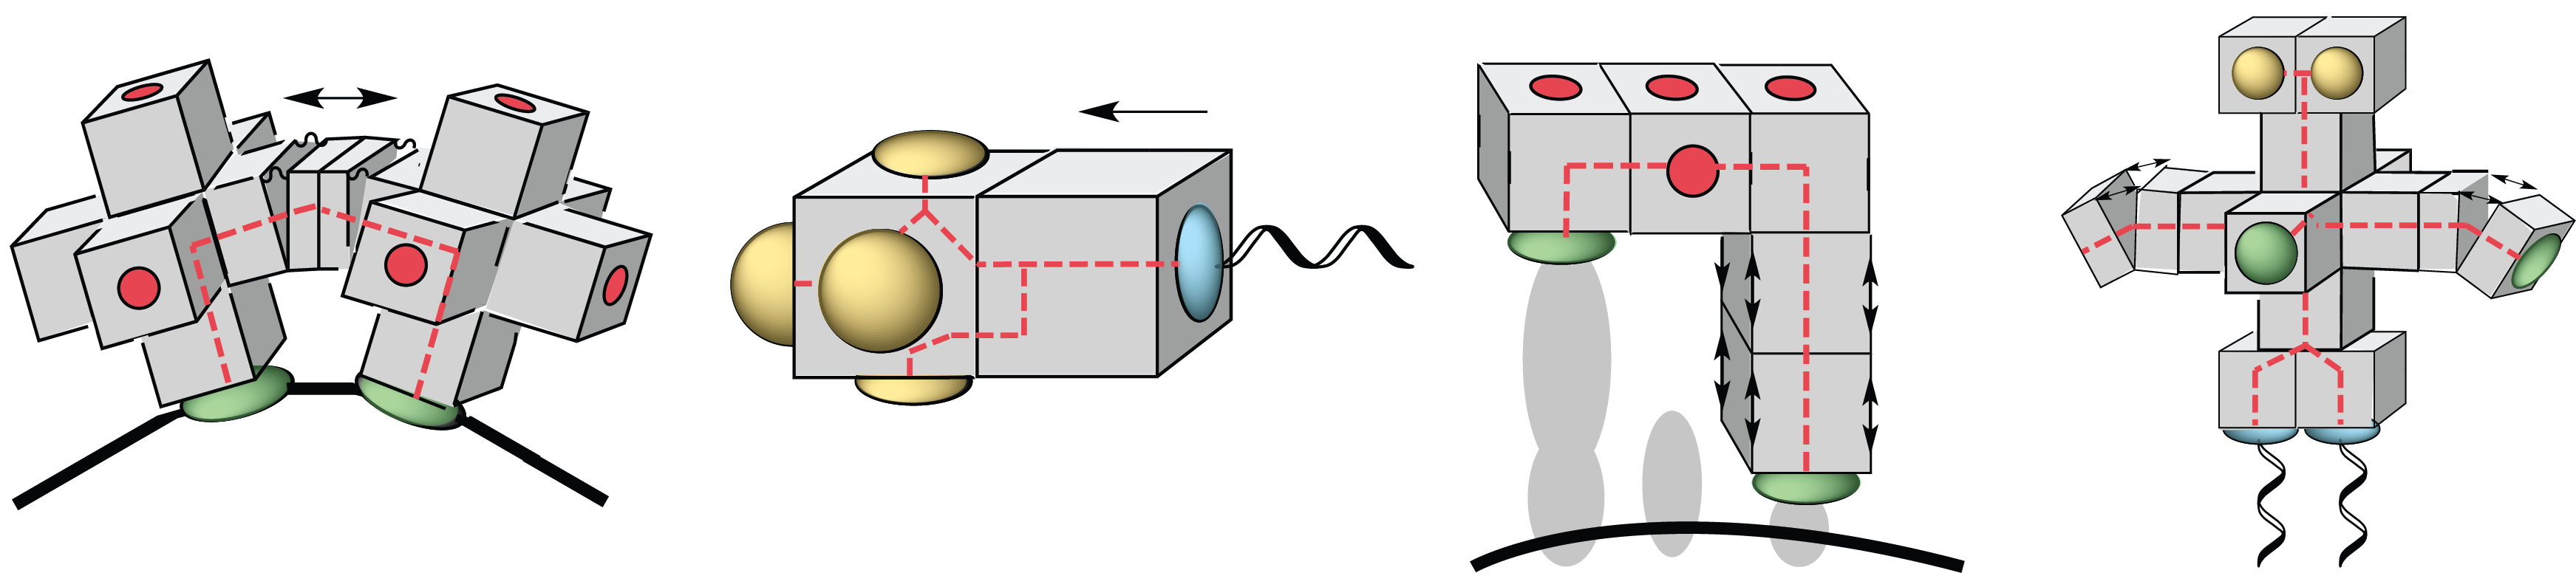
\includegraphics[width=\textwidth]{figures/dnaRoboticsHeader.png} 
    \caption{The original DNA Robotics design concept. The nanorobots are assembled from standardised cubic modules that functions as sensor, actuators, processors, or structural components. Image adapted from \url{https://dna-robotics.eu/about/}}
    \label{fig:dnaRoboticsHeader}
\end{figure}

As such, my contribution to the network and the field will be a step further in the ongoing effort to find methods for organising matter on the nanoscale.

\section{Thesis aim}
The aim of this thesis is to present methods that make it easier to design self-assembling nanostructures. This corresponds to the question of how to find the proper building blocks to use, but my aim has also been to simplify the detailed design of individual components. The next section will cover how the results of these two topics are documented.


\section{Thesis structure}
The thesis covers two related projects, both concerning the design and modular self-assembly of nanostructures. Each project is introduced by a separate chapter on its background, with Chapter~\ref{ch:polycubes_intro} introducing the first project and Chapter~\ref{ch:oxview_intro} introducing the second.

\paragraph{Modular self-assembly}
The first project covers the results of an abstract self-assembly model called \emph{polycubes}. Chapter~\ref{ch:polycubes_intro} introduces the project, providing a background to past experimental and theoretical self-assembly results. This includes an introduction to DNA origami, which is also relevant for the second project. Chapter~\ref{ch:polycubes1} then details the polycube model and the shapes we get when randomly sampling the input space. Chapter~\ref{ch:polycubes2} presents the results on the inverse problem: given a polycube shape, which input rules will assemble it and what is the least complex input?

\paragraph{Nucleic acid design, simulation, and visualisation}
The second project takes a more detailed view of self-assembly, with Chapter~\ref{ch:oxview_intro} providing background on computer-aided design tools for nucleic acid structures, together with some related simulation models. Chapter~\ref{ch:oxview} presents my contributions to \emph{oxView}, a web-based tool for the visualisation, design, and integration of DNA, RNA and protein structures.

\paragraph{}
Chapter~\ref{ch:conclusion} provides some concluding remarks, with a discussion on the results of both projects.

%Before moving on to the individual projects, however, the following sections will provide a general background on nucleic acid self-assembly and complexity.

%\section{Scope of the thesis}


%\begin{savequote}[8cm]
%Simplicity is prerequisite for reliability.
%  \qauthor{--- Edsger W. Dijkstra}
%\end{savequote}

\chapter{An introduction to modular assembly}
\label{ch:polycubes_intro}

\minitoc

This chapter will provide a background on modular self--assembly, starting with an explanation of how nucleic acids can be used as a building material and followed by examples of experimentally realised multicomponent structures. The final section will cover relevant self--assembly theory, presenting tile assembly models and their results.

%Components that self--assemble into such chrystals can also assemble bounded structures, if only a way can be found to make them self--limiting. 

\section{Nucleic acids as a building material}
Professor Ned Seeman was inspired to pioneer the field of \emph{structural DNA nanotechnology} after seeing the woodcut \emph{Depth} by M.C. Escher, where fish are depicted organised into a crystalline structure \cite{seeman_2016}. As it turned out, the nucleic acid strands of DNA (and later also RNA) could be designed to self--assemble into similar structures if the strand sequences were chosen cleverly enough, as this section will explain.

\subsection{DNA structures}

The main building material covered in this thesis is deoxyribonucleic acid (DNA). DNA is a linear polymer more known for encoding the genes of living systems \cite{calladine1997understanding}. Strands of DNA are made up of units called \emph{nucleotides}, consisting of a sugar--phosphate backbone unit, as well as one of four possible bases: \emph{adenine} (\textbf{A}), \emph{thymine} (\textbf{T}) \emph{cytosine} (\textbf{C}), and \emph{guanine} (\textbf{G}). 

Two strands of DNA can bind together to form a helical duplex. Through Watson--Crick base--pairing, the \textbf{A} nucleotide form two hydrogen bonds with \textbf{T}, while \textbf{G} forms three with \textbf{C}, making DNA double--stranded. Each strand has a directionality, conventionally represented as going from the 3' to the 5' end of the strand, making the duplex anti--parallel.

The base part of the nucleotide is hydrophobic, while the sugar--phosphate backbone is hydrophilic, which means that the bases ``hide'' on the inside of the duplex to avoid contact with water molecules. However, the length of a backbone unit is about 6~Å (0.6~nm), while the bases would need to be at a distance of 3.3~Å (the Van der Waals contact separation) to stack stably (without any room for water) \cite{calladine1997understanding}. To reconcile this inequality, the DNA duplex forms a double--helical structure with a radius of about 9~Å.

While an unbranched double--helix is the most natural confirmation, it is still possible for duplicates to branch into multiple junctions. For example, the Holliday junction is a junction between four double--helical arms, shown in Figure~\ref{fig:holliday} in one of its possible configurations.

\begin{figure}
    \centering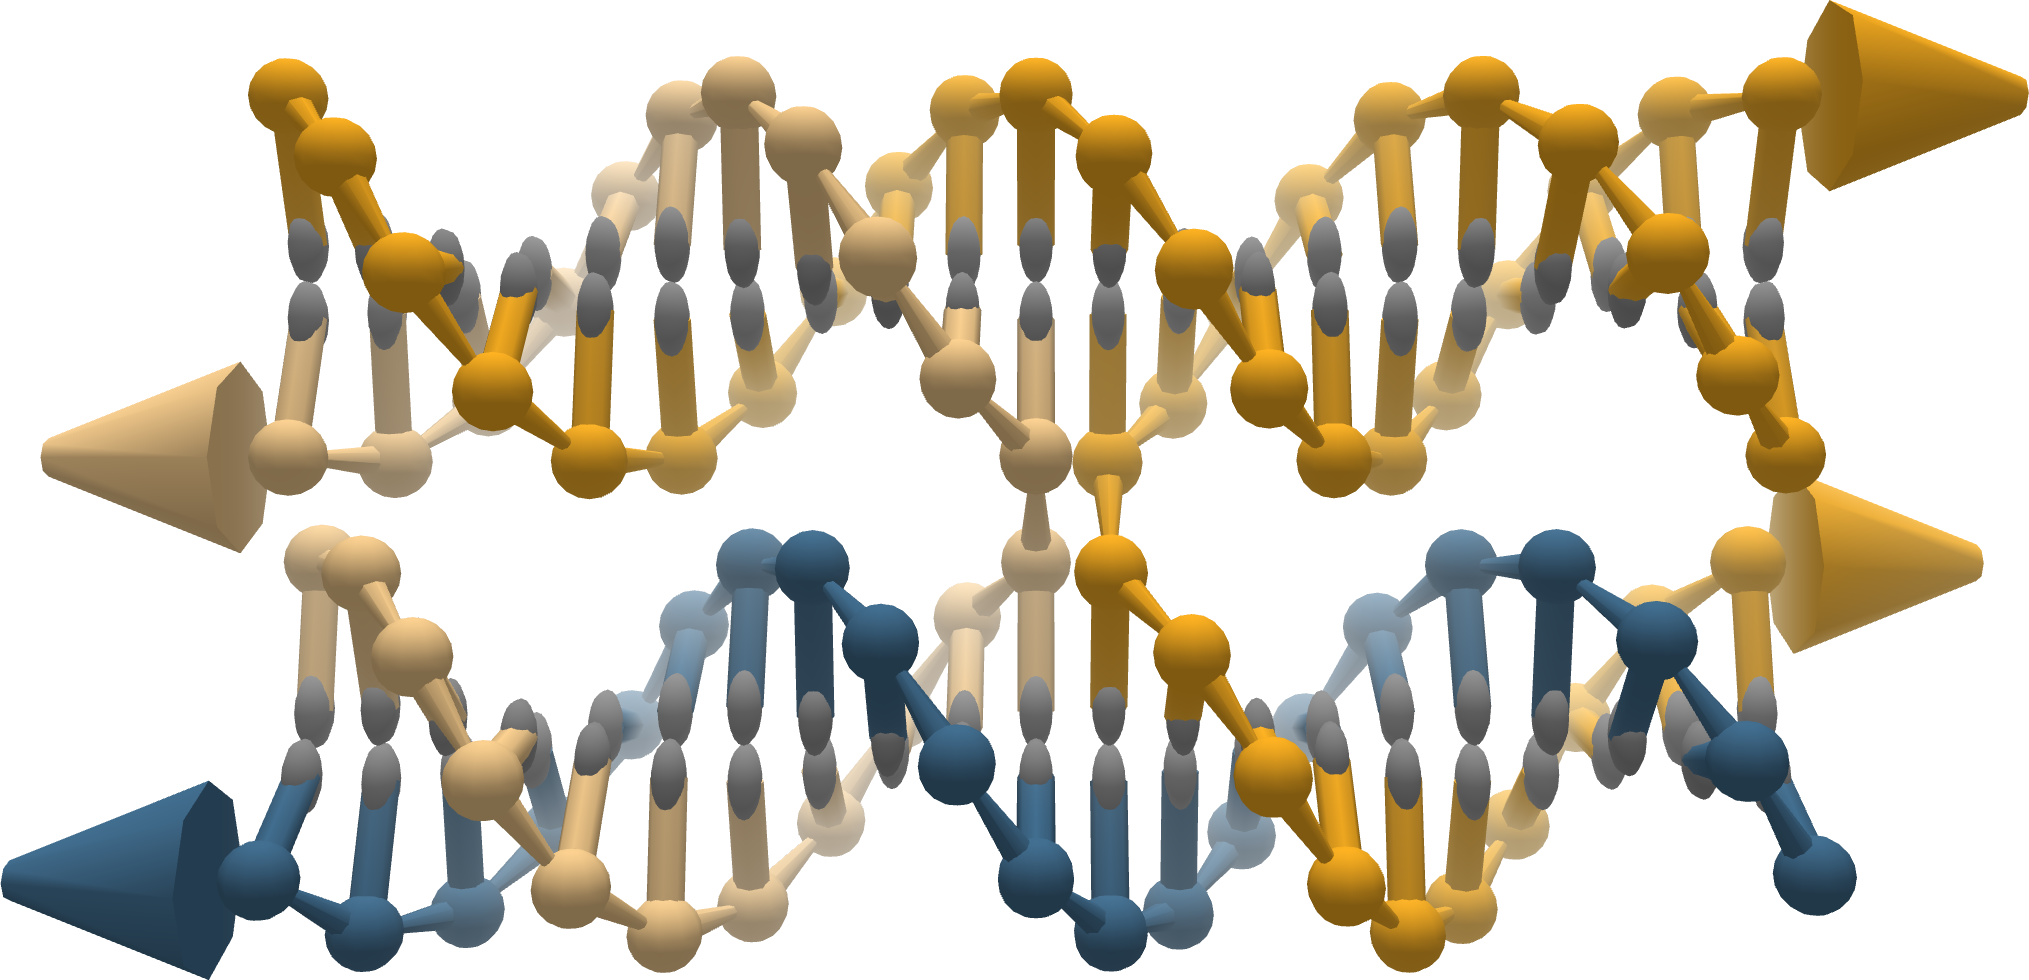
\includegraphics[width=\textwidth]{figures/holliday.png}
    \caption{Holliday junction, designed in oxView. Sugar--phosphate backbone unit are represented as spheres, while bases are represented as gray spheroids (here without any visual distinction between base types). Arrow heads at the end indicate the 3' end of each of the four strands.}
    \label{fig:holliday}
\end{figure}

%https://www.rcsb.org/structure/1M6G

%Double--stranded DNA has a persistence length of approximately [], while single--stranded sections are much more flexible,

By designing sequences with complementary domains corresponding to intended duplex regions, it is possible to create many different DNA motifs and structures \cite{seeman_2016, Seeman1982}, an understanding that pioneered the field of structural DNA nanotechnology and the use of DNA as a building material.

%% Add more here

Another breakthrough in the field was the DNA origami technique \cite{rothemund2006folding}, a now popular and proven method for creating larger irregular structures using DNA. The principle behind it, as illustrated in Figure~\ref{fig:dnaOrigami}, is to use short staple strands, each with one or more domans that are complementary to domains on a viral scaffold strand. As the temperature is gradually lowered, the staples bind to the scaffold as seen in Figure~\ref{fig:dnaOrigami}. If done correctly, this ``folds'' the scaffold into the desired structure, hence the name ``origami''. However, care must be taken to how the scaffold should be routed through the design to avoid kinetic traps where the folding cannot be completed.

With improved design software, it is becoming easier to design DNA origami structures of any given form. See Section~\ref{sec:design_tools} for an introduction to such tools.

% Andrew: I suggest a more extensive discussion of the basis of origami design to accompany an improved/alternate fig:{dnaOrigami}

% Some more added

\begin{figure}
    \centering
    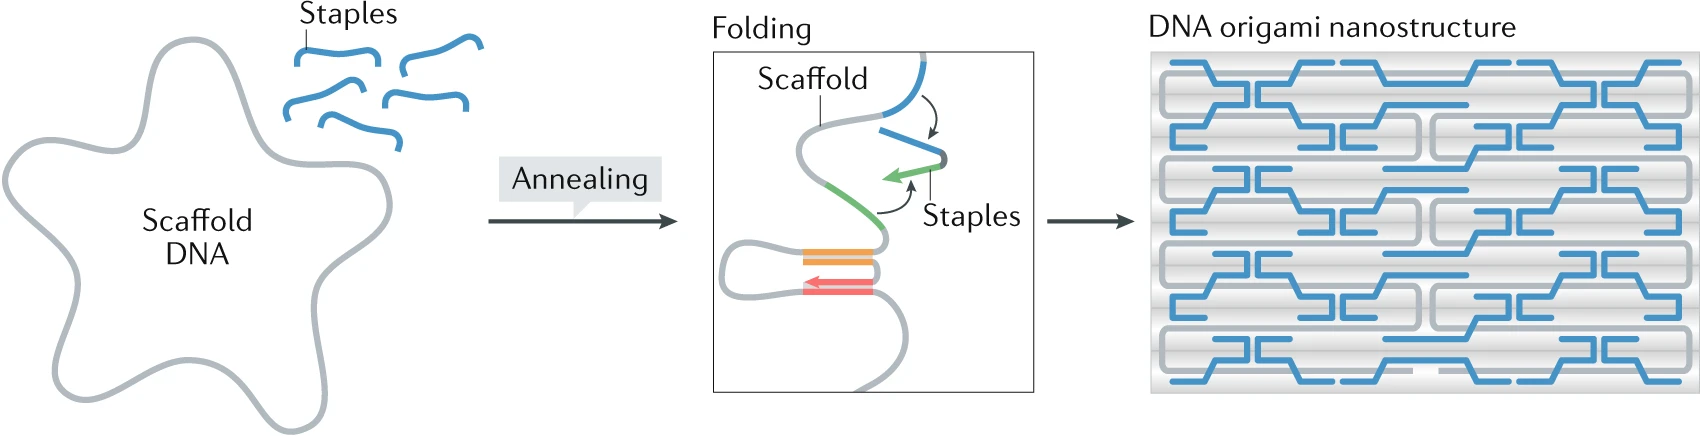
\includegraphics[width=\textwidth]{figures/dna_origami.png}
    \caption{Illustration of \emph{DNA origami} \cite{rothemund2006folding}, adapted from \cite{dey2021dna}. A long scaffold strand, obtained from a virus, is folded into the desired nanostructure by multiple short staple strands binding to complementary domains of the scaffold.
    }
    \label{fig:dnaOrigami}
\end{figure}

In DNA origami, the size of the structure is limited by the length of the scaffold, which motivates researchers to investigate approaches with multiple origami modules. Some previous results will be described in Section~\ref{sec:experimental_appl}. The work described in this thesis aims to simplify the design process significantly.

\subsection{RNA structures}
\label{sec:RNA_design}
Another promising building material for self--assembly is ribonucleic acid (RNA). RNA is very similar to DNA, but with a backbone containing the sugar ribose, instead of the deoxyribose sugar found in DNA, and with the \emph{thymine} base (\textbf{T}) replaced by \emph{uracil} (\textbf{U}).

Biologically, DNA is transcribed into RNA by the RNA polymerase enzyme as part of gene expression \cite{sadava2014life}. While DNA folding is easier to predict, the more reactive RNA backbone offers the possibility of a more functionalised structure; for example, by incorporating aptamers, enzymes, and other such modifications \cite{guo2010emerging}.

% TODO from Andrew: Check the above paragraph

In 2014, Geary et al., from the Andersen lab in Aarhus, demonstrated a method \cite{geary2014single, sparvath2017computer, geary2021rna} for co--transcriptionally folded RNA origami, which also enables folding \emph{in vivo}. As shown in Figure~\ref{fig:rna_origami}, the design used a set of tertiary RNA motifs (such as kissing hairpins and double crossovers) as modules. These modules are combined to generate a blueprint for a single strand, enforcing the desired self--interactions. Finally, an iterative algorithm is used to find a sequence that should co--transcriptionally fold into the intended shape.

\begin{figure}[h]
  \centering
  \begin{overpic}[width=\textwidth]{figures/rna_origami.png}
      \put(0,600){a)}
      \put(0,250){b)}
      \put(0,110){c)}
      \put(510,600){d)}
      \put(510,430){e)}
      \put(510,310){f)}
      \put(510,150){g)}
  \end{overpic}
  \caption{Co--transcriptional folding of RNA origami, adapted from \cite{geary2021rna}. \textbf{a)} The set of RNA motifs used as modular building blocks. \textbf{b)} Schematic of the modules connected to form a single strand. \textbf{c)} Atomistic model of the design in b). \textbf{d)} Shows the text--based blueprint used to create designs, while \textbf{e)}, \textbf{f)}, and \textbf{g)} shows scripts developed to aid the visualisation and preform sequence design for the origami.}
  \label{fig:rna_origami}
\end{figure}

The Andersen lab is one of the partners of the ITN network I am part of, and I have spent a two--month secondment there working with their RNA origami method. Some of my results on simulating RNA designs are covered in Section~\ref{sec:converting_rna_origami}.

% Andrew: A description of how RNA design is different (different helical structure & why it matters, single--stranded vs. multiple strands)

% "The emerging field of RNA nanotechnology might seem more promising in this regard because RNA is readily transcribed into a single strand in cells, which can be directly folded into a programmed nanostructure"
% https://www.nature.com/articles/nnano.2011.187


\section{Examples of modular nucleic acid structures} \label{sec:experimental_appl}
From small tiles made from a handful of strands to megadalton--scale structures made from multiple origami designs, modular self--assembly has seen considerable experimental research. This section provides a quick overview of some results of particular interest to the polycube model presented in Chapter~\ref{ch:polycubes1}.


\subsection{DNA tiles}
\label{sec:dna_tiles_bricks}
Following early nucleic acid multi--arm junctions and lattices suggested by Seeman \cite{seeman1982nucleic}, Winfree \cite{winfree1998algorithmic, winfree1998design} used double--crossover (DX) motifs, shown in Figure~\ref{fig:dna_tiles}.a, to self--assemble 2D DNA crystals. 
% Andrew: Describe how 4 sticky ends govern ?sossably?
The tiles attach using so--called \emph{sticky ends} where, as seen in Figure~\ref{fig:dna_tiles}.a, one of the strands continue past the end of a duplex region. Each tile has four such sticky ends, so it can can connect to four other tiles (as seen in Figure~\ref{fig:dna_tiles}.b) if their respective sticky end regions have complementary sequences. Also seen in Figure~\ref{fig:dna_tiles}.b, the lattices could be made with varying complexity, exemplified using either two or four different species of tiles.
% Tiles: https://www.nature.com/articles/28998

\begin{figure}[h]
  \centering
  \begin{overpic}[width=0.7\textwidth]{figures/dna_tiles.png}
    \put(0,450){a)}
    \put(0,240){b)}
  \end{overpic}
  \caption{DX tiles forming 2D lattices, adapted from \cite{winfree1998design}. \textbf{a)} Examples of tile designs with double--crossover motifs. \textbf{b)} Lattices made using two and four tile species respectively.}
  \label{fig:dna_tiles}
\end{figure}

\subsection{RNA tiles}

% Andrew: Other RNA structures?

%https://www.science.org/doi/abs/10.1126/science.1253920 
As already covered in Section~\ref{sec:RNA_design}, it is possible to co--transcriptionally fold \emph{RNA origami} \cite{geary2014single}. This was first shown in 2014 by Geary et al., who folded RNA tiles that connect through complementary 120-degree kissing loop interactions, as seen in Figure~\ref{fig:rna_tiles}, forming a hexagonal lattice. A significant promise with co--transcriptionally folded RNA structures is that they can be assembled \emph{in vivo} \cite{guo2010emerging}, with a DNA gene being transcribed into RNA inside a cell.

\begin{figure}[h]
  \centering
  \begin{overpic}[width=\textwidth]{figures/rna_tiles.jpeg}
      \put(0,300){a)}
      \put(320,300){b)}
      \put(750,300){c)}
  \end{overpic}
  \caption{Co--transcriptional folding RNA origami tiles, adapted from \cite{geary2014single}. The tiles connect through 120-degree kissing loop interactions, forming a hexagonal lattice. \textbf{a)} Detailed scematic of the four--helix 4H--AO tile. \textbf{b)} Co--transcriptional folding, where the RNA tile folds as it is transcribed from a DNA template. \textbf{c)} Hexagonal lattice formed by folded tiles.}
  \label{fig:rna_tiles}
\end{figure}

\subsection{DNA bricks}
% Bricks: https://www.nature.com/articles/nature24648

A three--dimensional DNA ``canvas'' was created in 2017 by Ong et al. \cite{ong2017programmable}, using a technique called \emph{DNA bricks}. Structures were assembled from up to about 30,000 unique components, as seen in Figure~\ref{fig:dna_bricks}. 
Each ``brick'' component consists of a single, 52 nucleotides long, DNA strand. The strand has four 13-nucleotide domains, each complementary domains to a domain in a neigbouring brick. A 13-nucleotide helix corresponds to approximately 1.25 turns, creating a 90$^{\circ}$ dihedral angle between the bricks, as Figure~\ref{fig:dna_bricks}.a shows.

Since each brick is unique, custom shapes can be ``sculpted'' by leaving out the voxels (3D pixels) not required.



% Andrew: Again, a missed opportunity to describe what is going on (4x8-base domains - interactions with neighbours - helical repeat)


\begin{figure}[h]
  \centering
  \begin{overpic}[width=\textwidth]{figures/dna_bricks.png}
    \put(0,350){a)}
    \put(450,350){b)}
    \put(450,120){c)}
  \end{overpic}
  \caption{DNA bricks, adapted from \cite{ong2017programmable}. \textbf{a)} DNA brick structure, where each of the up to 30'000 unique components is a 52 nucleotide DNA strand. The strands connect through a 13 base pair complementary domain at a 90 degree dihedral angle. \textbf{b)} A cuboid, here shown with 10,000 components, corresponds to a 20,000 voxel canvas. \textbf{c)} Approximating the shape of a teddy bear by removing a subset of the voxels from the canvas.}
  \label{fig:dna_bricks}
\end{figure}

\subsection{Finite DNA origami arrays}
\label{sec:origamiArrays}
% https://www.nature.com/articles/nature24655

In 2017, Tikhomirov et al. \cite{tikhomirov2017fractal, tikhomirov2017programmable} used the DNA origami technique to demonstrate two--dimensional patterns assembled on the micrometre--scale using square tiles where each tile was a complete origami, as seen in Figure~\ref{fig:origamiArrays}. The tiles connect to each other through complementary single--stranded overhangs on their edges.

The patterns could either be hierarchically assembled from unique tiles \cite{tikhomirov2017fractal} or assembled into random patterns from a small number of tile types \cite{tikhomirov2017programmable}. The binding strength could be adjusted using a variable amount of edge overhangs, as seen in Figure~\ref{fig:origamiArrays}.b). Arrays up to \(8 \times 8\) tiles were successfully produced, although larger arrays had a much smaller yield (Figure~\ref{fig:origamiArrays}.c).

While the random tilings were generally unbounded, Tikhomirov et al. also showed how to program a finite grid, as seen in Figure~\ref{fig:origamiArrays}.d). These tiles are very similar to the polyomino model later described in Section~\ref{sec:polyomino}.

\begin{figure}[h]
  \centering
  \begin{overpic}[width=\textwidth]{figures/monalisa_tiles.png}
    \put(-20,580){a)}
    \put(200,580){b)}
    \put(-20,150){c)}
    \put(600,580){d)}
  \end{overpic}
  \caption{DNA origami arrays, adapted from \cite{tikhomirov2017fractal, tikhomirov2017programmable}. \textbf{a)} Strand--level diagram of a \(12 \times 12\) version of the the origami tile (actual size is \(22 \times 22\) helices). \textbf{b)} \(4 \times 4\) tile ``Mona Lisa'' pattern. The pattern is achieved through double--stranded extensions of selected staple strands inside each origami tile. Staples with the extension correspond to pixels turned on, while those without are turned off. \textbf{c)} AFM image of patterned assemblies of different sizes (left) with their respective yields (right). \textbf{d)} Abstract design diagrams (left) and AFM images (right) of finite origami arrays, designed to different sizes \cite{tikhomirov2017programmable}.}
  \label{fig:origamiArrays}
\end{figure}

\subsection{Shape--complementary origami}
\label{sec:shape-complementary}
% 2D https://www.nature.com/articles/nchem.1070
% 3D https://science.sciencemag.org/content/347/6229/1446.abstract

% Huge https://www.nature.com/articles/s41563-021-01020-4

Also in 2017, Wagenbauer et al. \cite{wagenbauer2017gigadalton} used shape--complementarity to assemble DNA origami components into three--dimensional polyhedral shapes up to 450 nanometers in diameter. Later, in 2021, Sigl et al. assembled large shells from shape--complementary origami triangles, as seen in Figure~\ref{fig:shape-complementarity}. The triangular sides attach through protrusions and indentations of complementary shape, as seen in Figure~\ref{fig:shape-complementarity}.a). By having extra helices protruding from one triangle side, and a hole with a shape they would fit on the side of another triangle, the two components can binding together through stacking interactions at the helix ends, a method first shown by Woo et al. \cite{woo2011programmable}.

While the described experiments use triangular components, the general shape--complementary assembly method is a relevant option for a physical realization of the torsionally rigid polycube patches described in Chapter~\ref{ch:polycubes1}.

\begin{figure}[h]
  \centering
  \begin{overpic}[width=\textwidth]{figures/icosahedral_shell.png}
    \put(0,320){a)}
    \put(620,320){b)}
  \end{overpic}
  \caption{Shape--complementary triangles assembling polyhedral shells. Adapted from \cite{sigl2021programmable}. \textbf{a)} Polyhedral shell design for T=9. \(N\) is the triangulation number (the number of unique edges required for assembly), \(\alpha\) is the bevel angle of the triangle sides, and \(N\) is the number of triangles required for a full shell. \textbf{b)} Cryo--EM reconstruction of an assembled T=4 icosahedral shell.}
  \label{fig:shape-complementarity}
\end{figure}


\subsection{DNA origami nanochambers}
% https://pubs.acs.org/doi/full/10.1021/jacs.0c07263

In 2020, Lin et al. \cite{nano-chambers_lin2020} presented cubic DNA origami ``nanochambers''. The chambers have sticky--end overhangs on every side of the cube, allowing it to assemble in one, two and three dimensions, as can be seen in Figure~\ref{fig:nanochambers}. However, since the shape is only rotationally symmetric around the z--axis, the assembly is a still only a limited subset of the polycube model described in Chapter~\ref{ch:polycubes1}. 

\begin{figure}[h!]
  \centering
  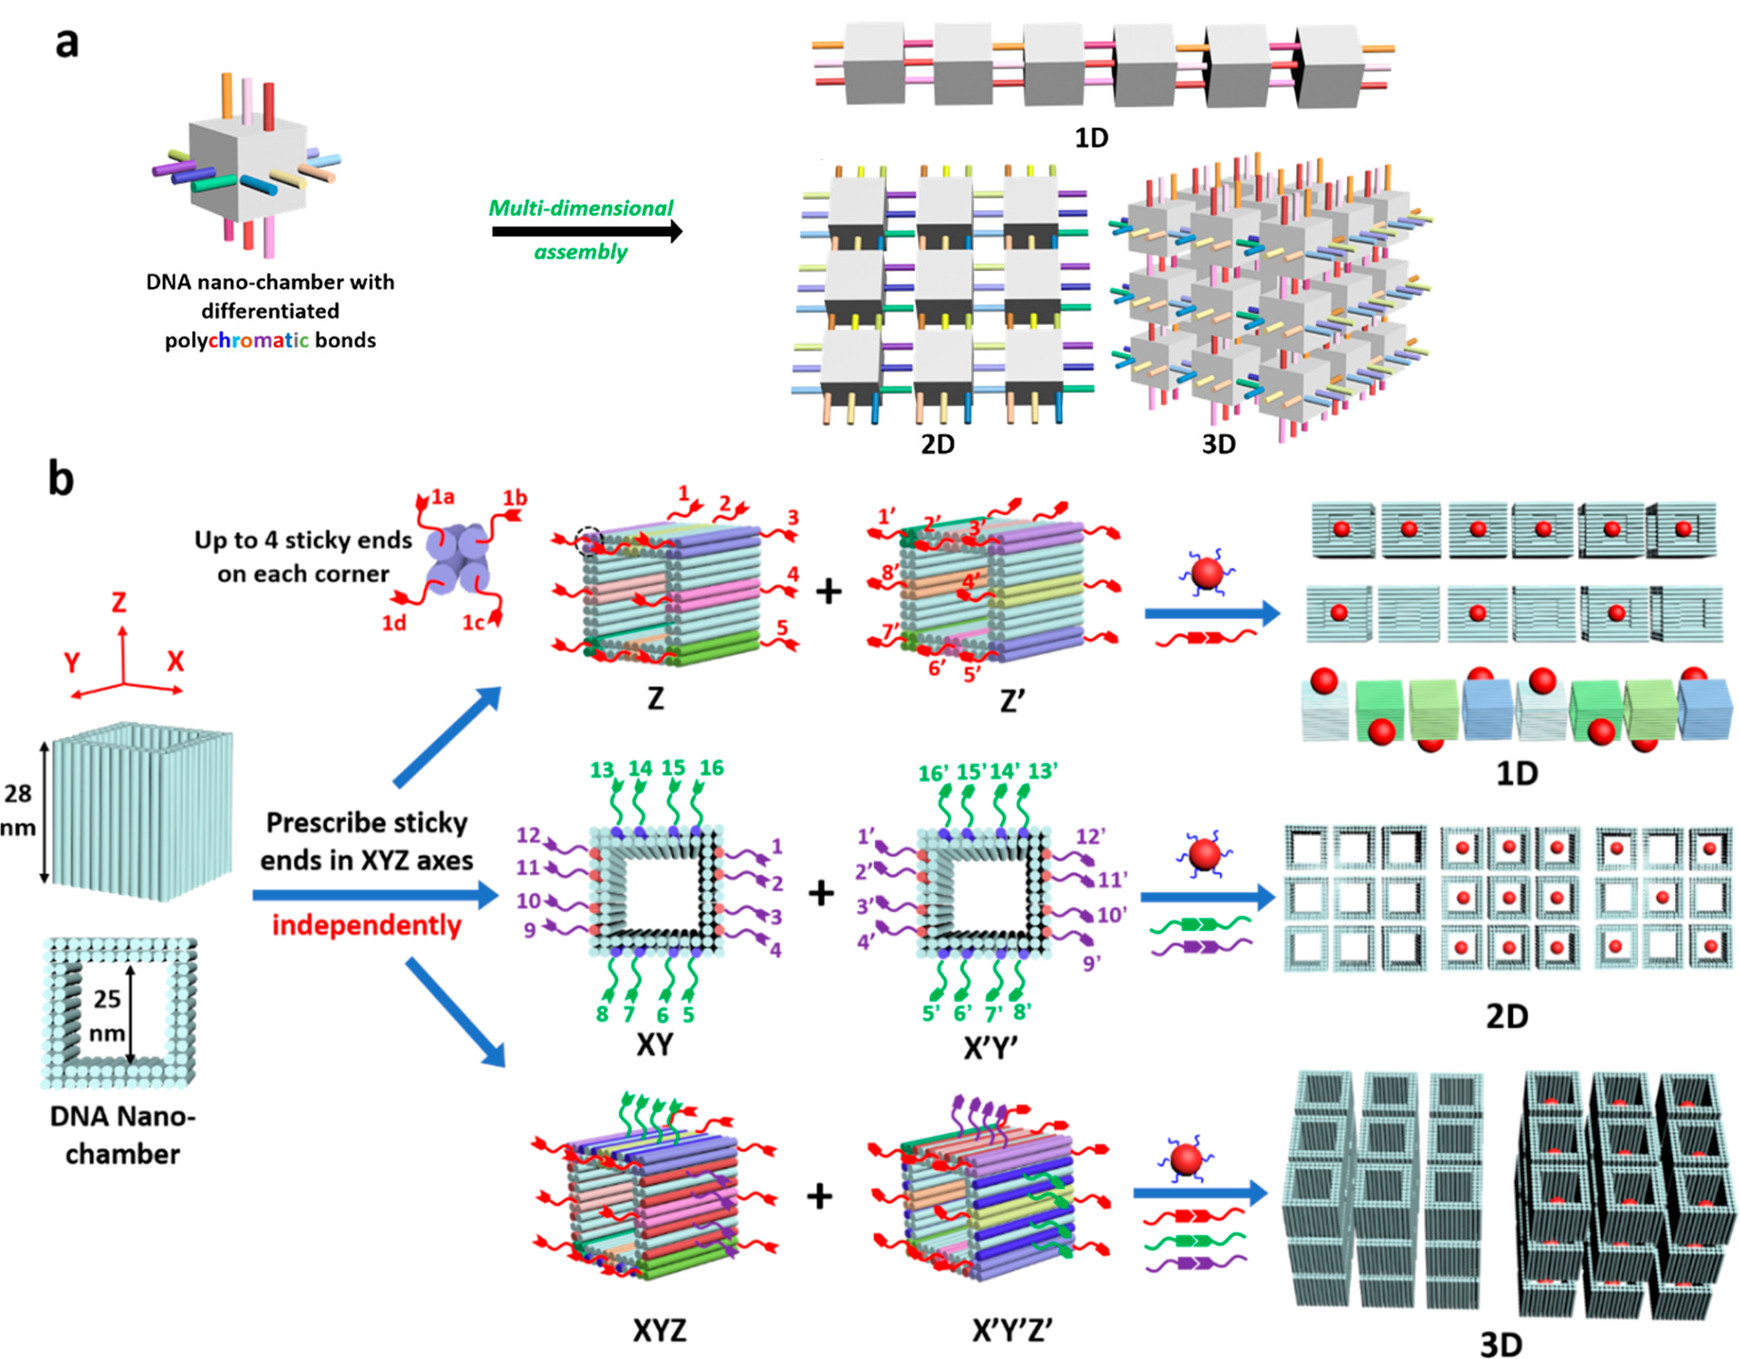
\includegraphics{figures/nanochambers2.jpeg}
  \caption{DNA origami nanochambers, adapted from \cite{nano-chambers_lin2020}. \textbf{a)} Concept illustration, where building blocks with \emph{polychromatic} bonds (differentiated though different single--stranded sequences), assemble into 1D, 2D, and 3D structures. \textbf{b)} Schematic of DNA nanochamber programmable assembly, showing sticky end overhangs applied in 1D, 2D, and 3D assemblies.}
  \label{fig:nanochambers}
\end{figure}

\subsection{Octahedral DNA origami frames}
In 2020, Wang et al. \cite{tian_octahedra2020} showed how octahedral DNA origami frames could be used as building blocks in limited and unlimited programmed assemblies, as seen in Figure~\ref{fig:tian_octahedra}. Using sticky--end overhangs at the octahedral vertices, the building blocks have the connectivity, as well as the rotational symmetry, of a cube.

Due to the flexibility of the single--stranded connections, the connections are less torsionally rigid than assumed in the polycube model, later described in Chapter~\ref{ch:polycubes1}. However, as can be seen in Figure~\ref{fig:tian_octahedra}, shapes such as the cube can still be assembled with good yield.

% https://onlinelibrary.wiley.com/doi/abs/10.1002/anie.201913958

\begin{figure}[!h]
  \centering
  \begin{overpic}[width=\textwidth]{figures/tian.jpg}
    \put(0,480){a)}
    \put(280,480){b)}
    \put(670,480){c)}
  \end{overpic}
  \caption{Octahedral DNA origami frames, adapted from \cite{tian_octahedra2020}. \textbf{a)} Two octahedra with complementary sticky ends binding together to form a dimer. The edges consist of six--helix bundles. \textbf{b)} nanoclusters assembled from different sets of building blocks. \textbf{c)} \(2 \times 2 \times 2 \) cube nano cluster (top) and histogram of the mass fraction, where the intended design of eight components per cluster is the most common.}
  \label{fig:tian_octahedra}
\end{figure}


\FloatBarrier
\section{Theory of modular self--assembly}

With some experimental background covered, let us now look at the progress on the theoretical side of self--assembly design. Although the designs covered are built from nucleic acid strands, it would be computationally impractical to include that level of detail in a self--assembly model. A more straightforward approach is instead to model each component as a discrete tile on a lattice. This section will present earlier such models as a background to my own polycube model, which will be introduced in Chapter~\ref{ch:polycubes1}.

For all modular designs, an important factor is the number of unique components needed. This relates to the concept of complexity covered in Section~\ref{sec:AIT}.

\subsection{Wang tiles}
Introduced by Hao Wang in 1961 \cite{wang1961proving}, \emph{Wang tiles} are square tiles with a colour assigned to each of their four edges. Without rotating or reflecting the tiles, they assemble so that adjacent edges have the same colour.

%\begin{figure}[h]
 % \centering\includesvg[width=0.5\textwidth]{figures/Wang_11_tiles.svg}
 % \caption{Wang tiles}on
%\end{figure}

The DNA tiles by Winfree et al. \cite{winfree1998design}, presented in Section~\ref{sec:dna_tiles_bricks}, behave like Wang tiles by design and do not allow rotations or reflections. Winfree investigated the possibility of using such tiles for computation \cite{winfree1998algorithmic}, which led to aTAM: the algorithmic Tile Assembly Model.

\subsection{The algorithmic tile assembly model}
\label{sec:atam}
% David Doty overview: https://cacm.acm.org/magazines/2012/12/157881-theory-of-algorithmic-self-assembly/fulltext

% Molecular algorithms https://www.nature.com/articles/s41586-019-1014-9

The algorithmic Tile Assembly Model (aTAM), shown in Figure~\ref{fig:atam}, models the dynamic behaviour of the double crossover DNA tiles introduced by Winfree et al. \cite{winfree1998design}. Each tile has four patches, one on each edge, corresponding to the four sticky ends of the DNA tile. Furthermore, the patches can have different strengths, with a global temperature variable determining the total connection strength required for a tile to attach \cite{doty2012theory}.

In the example seen in Figure~\ref{fig:atam}, the pattern grows from the initial bottom--right seed into the blue horizontal bottom row and the rightmost vertical column. This is because these tiles have ``strength-2'' glues with enough binding strength to attach by themselves \cite{doty2012theory}. The additional tiles have weaker ``strength-1'' glues (illustrated as thinner black connectors), so they need at least two complementary patches to achieve the binding strength threshold (temperature).

Because of this so--called \emph{co--operative binding}, the tiles can be seen as logic gates performing computation; given the bottom and right patches as input bits, the matching tile attaches and produces two computed output bits (top and left).

% Ard: You should mention that a key interest in this model is because it is thought to be Turing universal.


\begin{figure}[h]
  \centering\includesvg[width=\textwidth]{figures/atam.svg}
  \caption{Algorithmic self--assembly of a Sierpiński triangle. Adapted from \cite{doty2017}. A tile set (right) grows from an initial seed by co--operatively attaching self--complementary edges (without rotation). The \(0\) and \(0\) ``glues'' are weaker and require two matching bonds to attach (co--operative binding), compared to the \(W\) (west) and \(N\) (north) glues that are strong enough to bind alone.}
  \label{fig:atam}
\end{figure}

\subsection{The polyomino model}\label{sec:polyomino}

% Ard: I think you need a longer section on the background of the polyomino model here. This is very terse.

The main inspiration for the \emph{polycube} model (presented in Chapter~\ref{ch:polycubes1}) is the polyomino model \cite{ahnert2010self, johnston2011evolutionary}. As noted in Section~\ref{sec:origamiArrays}, the 2D model is similar in assembly to the later experimental micrometer scale tile designs by Tikhomirov \cite{tikhomirov2017programmable} shown in Figure~\ref{fig:origamiArrays}.d). Compared to the aTAM model described in Section~\ref{sec:atam}, polyomino tiles are allowed to rotate (but not invert), creating further possibilities for symmetries. Also, the edge binding is not self--complementary, with complementary colour pairs used instead. Finally, polyominoes have a constant binding strength, assembling irreversibly and without co--operative binding (corresponding to ``strength-0'' glues).

See Figure~\ref{fig:polyominoes} for an illustration of the model, where an input \emph{genotype} (describing the four possible tile types) is mapped into an assembled output polyomino phenotype by stochastically growing the shape from an initial seed. The growth stops if, as in the figure, no more tiles can attach (since the colour \(0\) does not bind to anything). If the growth is infinite, the genotype is called \emph{unbounded}. A genotype is considered \emph{deterministic} if it assembles the same phenotype polyomino every time. Only output corresponding to bounded and deterministic genotypes are considered valid.

\begin{figure}[h]
    \centering
    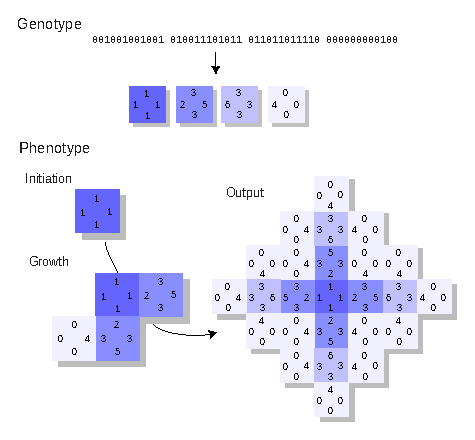
\includegraphics[width=0.6\textwidth]{figures/polyominoes.eps}
    \caption{Illustration of the polyomino assembly model, adapted from \cite{johnston2011evolutionary}. A \emph{genotype}, in the form of a ruleset of possible tiles, encodes for a polyomino \emph{phenotype}, grown stochastically from an initial seed tile. The integers on the tile edges represent the colour of that edge, where every even integer \(n\) binds to the odd \(n-1\). The exception is tile edges with the colour \(0\) that does not bind at all. The output phenotype is grown from an initial seed, a tile of the first species defined in the genotype. Additional tiles, from any species in the genotype, are then added wherever there are compatible edge colours.}
    \label{fig:polyominoes}
\end{figure}

\subsection{Algorithmic Information Theory and input-output maps}
\label{sec:AIT}
% https://www.ox.ac.uk/news/science-blog/%E2%80%98simplicity-bias%E2%80%99-science

% https://www.nature.com/articles/s41467-018-03101-6

% https://solo.bodleian.ox.ac.uk/permalink/f/89vilt/oxfaleph022417805

%Some things, whether in the form of a shape, a song, or a binary string, require less information to describe than others.

If we have a self--assembly model mapping from an input set of building blocks into an output shape, can we find the simplest input for a given output? To answer this, we first need to consider what we mean by ``simplest''; what is the \emph{complexity} of a shape?

Complexity has different definitions in different fields, but here we focus on the amount of information needed to describe something, in this case, a shape. Some things, whether in the form of a shape, a song, or a binary string, clearly require less information to describe than others, and we would then call those less complex than their counterparts, but how can we quantify that difference?

Let us first consider the complexity of text strings. If you have a monkey pressing random keys on a typewriter, you would expect it to produce every string of length \(N\) with equal probability (assuming the keystrokes were indeed truly random). With \(k\) keys on the keyboard, the probability for any string of length \(N\) is then \(k^{-N}\). For example, the title of this thesis, while unlikely to appear randomly, would be equally as probable as any other 50-character string, see the three example strings below, all with probability \(k^{-50}\):
\begin{lstlisting}[numbers=left]
  DESIGN AND MODULAR SELF--ASSEMBLY OF NANOSTRUCTURES
  SHWDRVWKFORWJDOEXOZLSBNREKC Z  VSDJJF  ROKFYRVMIUI
  AAAAAAAAAAAAAAAAAAAAAAAAAAAAAAAAAAAAAAAAAAAAAAAAAA
\end{lstlisting}

But what if we described our strings using algorithms, rather than a full listing of the letters it contains? For example, string number three above could, similarly to the others, then be described using the C programming language as the algorithm:

\begin{lstlisting}[language=c]
printf("AAAAAAAAAAAAAAAAAAAAAAAAAAAAAAAAAAAAAAAAAAAAAAAAAA");
\end{lstlisting}

But now, a much shorter description also exists:

\begin{lstlisting}[language=c]
for(int i=50; i--;) printf("A");
\end{lstlisting}

There are also a number of possible valid variations of the code above, with different variable names and coding conventions, all producing the same output. In other words, not only is the description shorter than writing out the full string but multiple inputs map to the same output, increasing the probability of that particular output further. It also feels intuitive that a string repeating a single letter should be less complex than a random--looking alternative, so this definition of complexity feels reasonable.

The concept of using the shortest possible computer program that can describe an object (for example, a binary string) to determine its complexity is central within the field of Algorithmic Information Theory (AIT) and is called \emph{Kolmogorov complexity} (or Solomonoff–Kolmogorov–Chaitin to give full credit) \cite{LiMing2019AitK}. More specifically, the Kolmogorov complexity \(K(x)\) of an output \(x\) is the length of the shortest program that generates \(x\) on a Universal Turing Machine (UTM) \cite{LiMing2019AitK}.

AIT also includes the \emph{coding theorem}, introducing lower and upper bounds for the probability \(P(x)\) of generating a binary string \(x\) as \(2^{-K(x)} \le P(x) \le 2^{-K(x) + \mathcal{O} (1)}\). In other words, low--complexity outputs are exponentially more likely to be generated by random input compared to high--complexity outputs. This could be compared to how there are many more programs generating the ``simple'' string number three above compared to the randomly generated string two or the carefully selected string one.

However, a problem with Komologrov complexity is that finding the shortest program for a given output is far from trivial (it is, in fact, \emph{uncomputable} in general, due to the \emph{halting problem} \cite{LiMing2019AitK}). Fortunately, Dingle at al \cite{dingle2018input} were able to derive an upper bound to the probability using a computable approximation \(\widetilde{K}(x)\) of the Komologrov complexity:

\[
  P(x) \lesssim 2^{-a\widetilde{K}(x) -b}
\]

The constants \(a\) and \(b\) depend on the input--output map used (but are independent of \(x\)). This is very helpful for calculating the complexity of self--assembled shapes, where properties of the simplest known input rule can be used as such a Komologrov complexity proxy, as will be seen in Section~\ref{sec:polyomino_evolve} and Chapter~\ref{ch:polycubes1}.

\subsection{Evolving polyominoes}
\label{sec:polyomino_evolve}

Evolutionary runs of polyominoes, where a genetic algorithm mutates a genotype population and selects surviving shapes depending on their size, showed a clear bias toward structures with low complexity and high symmetry \cite{johnston2021}. See Figure~\ref{fig:polyomino_symmetries}, where the frequency of protein complexes and polyominoes are compared to their complexity. The number of interface types required (number of patch colours in the polyomino case) is used as a proxy measure for the Komologrov complexity of the structure (see Section~\ref{sec:AIT}).

The evolutionary fitness of the polyominoes only depended on their size (16--mers had the highest fitness), so the simplicity was not selected for but is instead a property of the mapping. This finding is in line with the Algorithmic Information Theory arguments made by Dingle et al. \cite{dingle2018input}, who showed the same simplicity bias for a set of various input--output maps.

\begin{figure}[h]
  \centering
  \begin{overpic}[width=0.9\textwidth]{figures/polyomino_symm_and_simpl.eps}
    \put(0,750){a)}
    \put(520,750){b)}
    \put(0,590){c)}
    \put(520,590){d)}
  \end{overpic}
  \caption{Frequent symmetry and simplicity through evolution, adapted from \cite{johnston2021}. Both protein complexes (a) and polyominoes (b) self--assemble from individual units. \textbf{c)} Frequency of 6--mer protein complex topologies in the protein data bank, versus their complexity (measured as the number of interface types) \textbf{d)} Frequency versus complexity of polyominoes found in evolutionary runs with a fitness function seeking 16--mers.}
  \label{fig:polyomino_symmetries}
\end{figure}

\chapter{\label{ch:3-polycubes}Modular self-assembly of polycubes}

\minitoc

As introduced in the previous chapter, there is an increasing interest within the field of DNA nanotechnology to create finite-sized multi-component objects. While some coarse-grained tile models exists, there still remains a need for methods to quickly explore the assembly of multi-component 3D structures.
This chapter describes my polycube model and details how it can be used to sample a large amount of assembly rules, showing that some polycube shapes are significantly more common than others. The following chapter will show how to obtain the simplest assembly rule for any given polycube shape.

\section{The polycube model}
A polycube consists of a number of equally-sized cubes, connected by their neigbouring faces; a three-dimensional analogue to how polyominos are squares connected by their neigbouring edges. In the model presented here, a polycube is stochastically self-assembled according to a specified rule, where a rule is a set of available species. Each cube species describes a type of cube that can be present in the polycube; cubes belonging to the same species are always identical.

Each species has six patches; one on each face of the cube, and each patch has a "colour" and an orientation. The colour is indicated by a signed integer and the orientation is one of four possible rotations: 
\includegraphics[width=10pt]{figures/face.eps}\hspace{4pt}(\(0\)),
\begingroup\setbox0=\hbox{
\includegraphics[width=10pt,angle=-90]{figures/face.eps}}\parbox{\wd0}{\box0}\endgroup\hspace{4pt}(\(\frac{\pi}{2}\)),
\begingroup\setbox0=\hbox{
\includegraphics[width=10pt,angle=180]{figures/face.eps}}\parbox{\wd0}{\box0}\endgroup\hspace{4pt}(\(\pi\)) or
\begingroup\setbox0=\hbox{
\includegraphics[width=10pt,angle=90]{figures/face.eps}}\parbox{\wd0}{\box0}\endgroup\hspace{4pt}(\(\frac{3\pi}{2}\)). A patch can bind to another patch if and only if they have the opposite colour and the same orientation. If the patch color is zero, the patch is considered empty and will not bind to anything. The model can also be expanded to more complicated colour interaction matrices or changed to pair odd integers with each subsequent integer as in the polyomino model\cite{ahnert2010self}\cite{johnston2011evolutionary} described in Section \ref{sec:polyomino}.

The stochastic self-assembly of a polycube starts by placing a cube from one of the available species as a seed at the origin. If the assembly mode is set to be seeded, it will always use first species in of rule. If the assembly mode is stochastic, the species of the seed is chosen at random.

Each possible neighbour to the placed cube, given the cube's patches, is then added to a list of possible moves. For the next step, a possible move is chosen at random and the rule is searched in a random order for a species fitting the move. Cubes can be rotated to fit and if a fitting species is found, the corresponding cube is added. If there is no fit, the move is discarded. Moves are processed until the list of moves is empty or the polycube grows beyond a specified size, at which point it is considered unbounded.

To determine if the rule is deterministic, the assembly is repeated \(n_{times}\) times (default 10) and the outputs compared for equality (allowing rotation).

ADD FIGURE ABOUT DETERMINISTIC AND UNBOUNDED ASSEMBLIES!!

It could be argued, instead of first picking a random move and then randomly trying all available species to find a fit, that one should pick both a move and a species at random until a fit is found. While this would take longer time, it would avoid biasing the assembly toward unlikely assembly results, where a move is picked that would otherwise usually be blocked by more likely surrounding cubes. However, since only deterministic and bounded rules are of interest, this would only affect the end result in the cases where the bias is strong enough and \(n_{times}\) is low enough to falsely make the rule seem deterministic.

\begin{figure}
\centering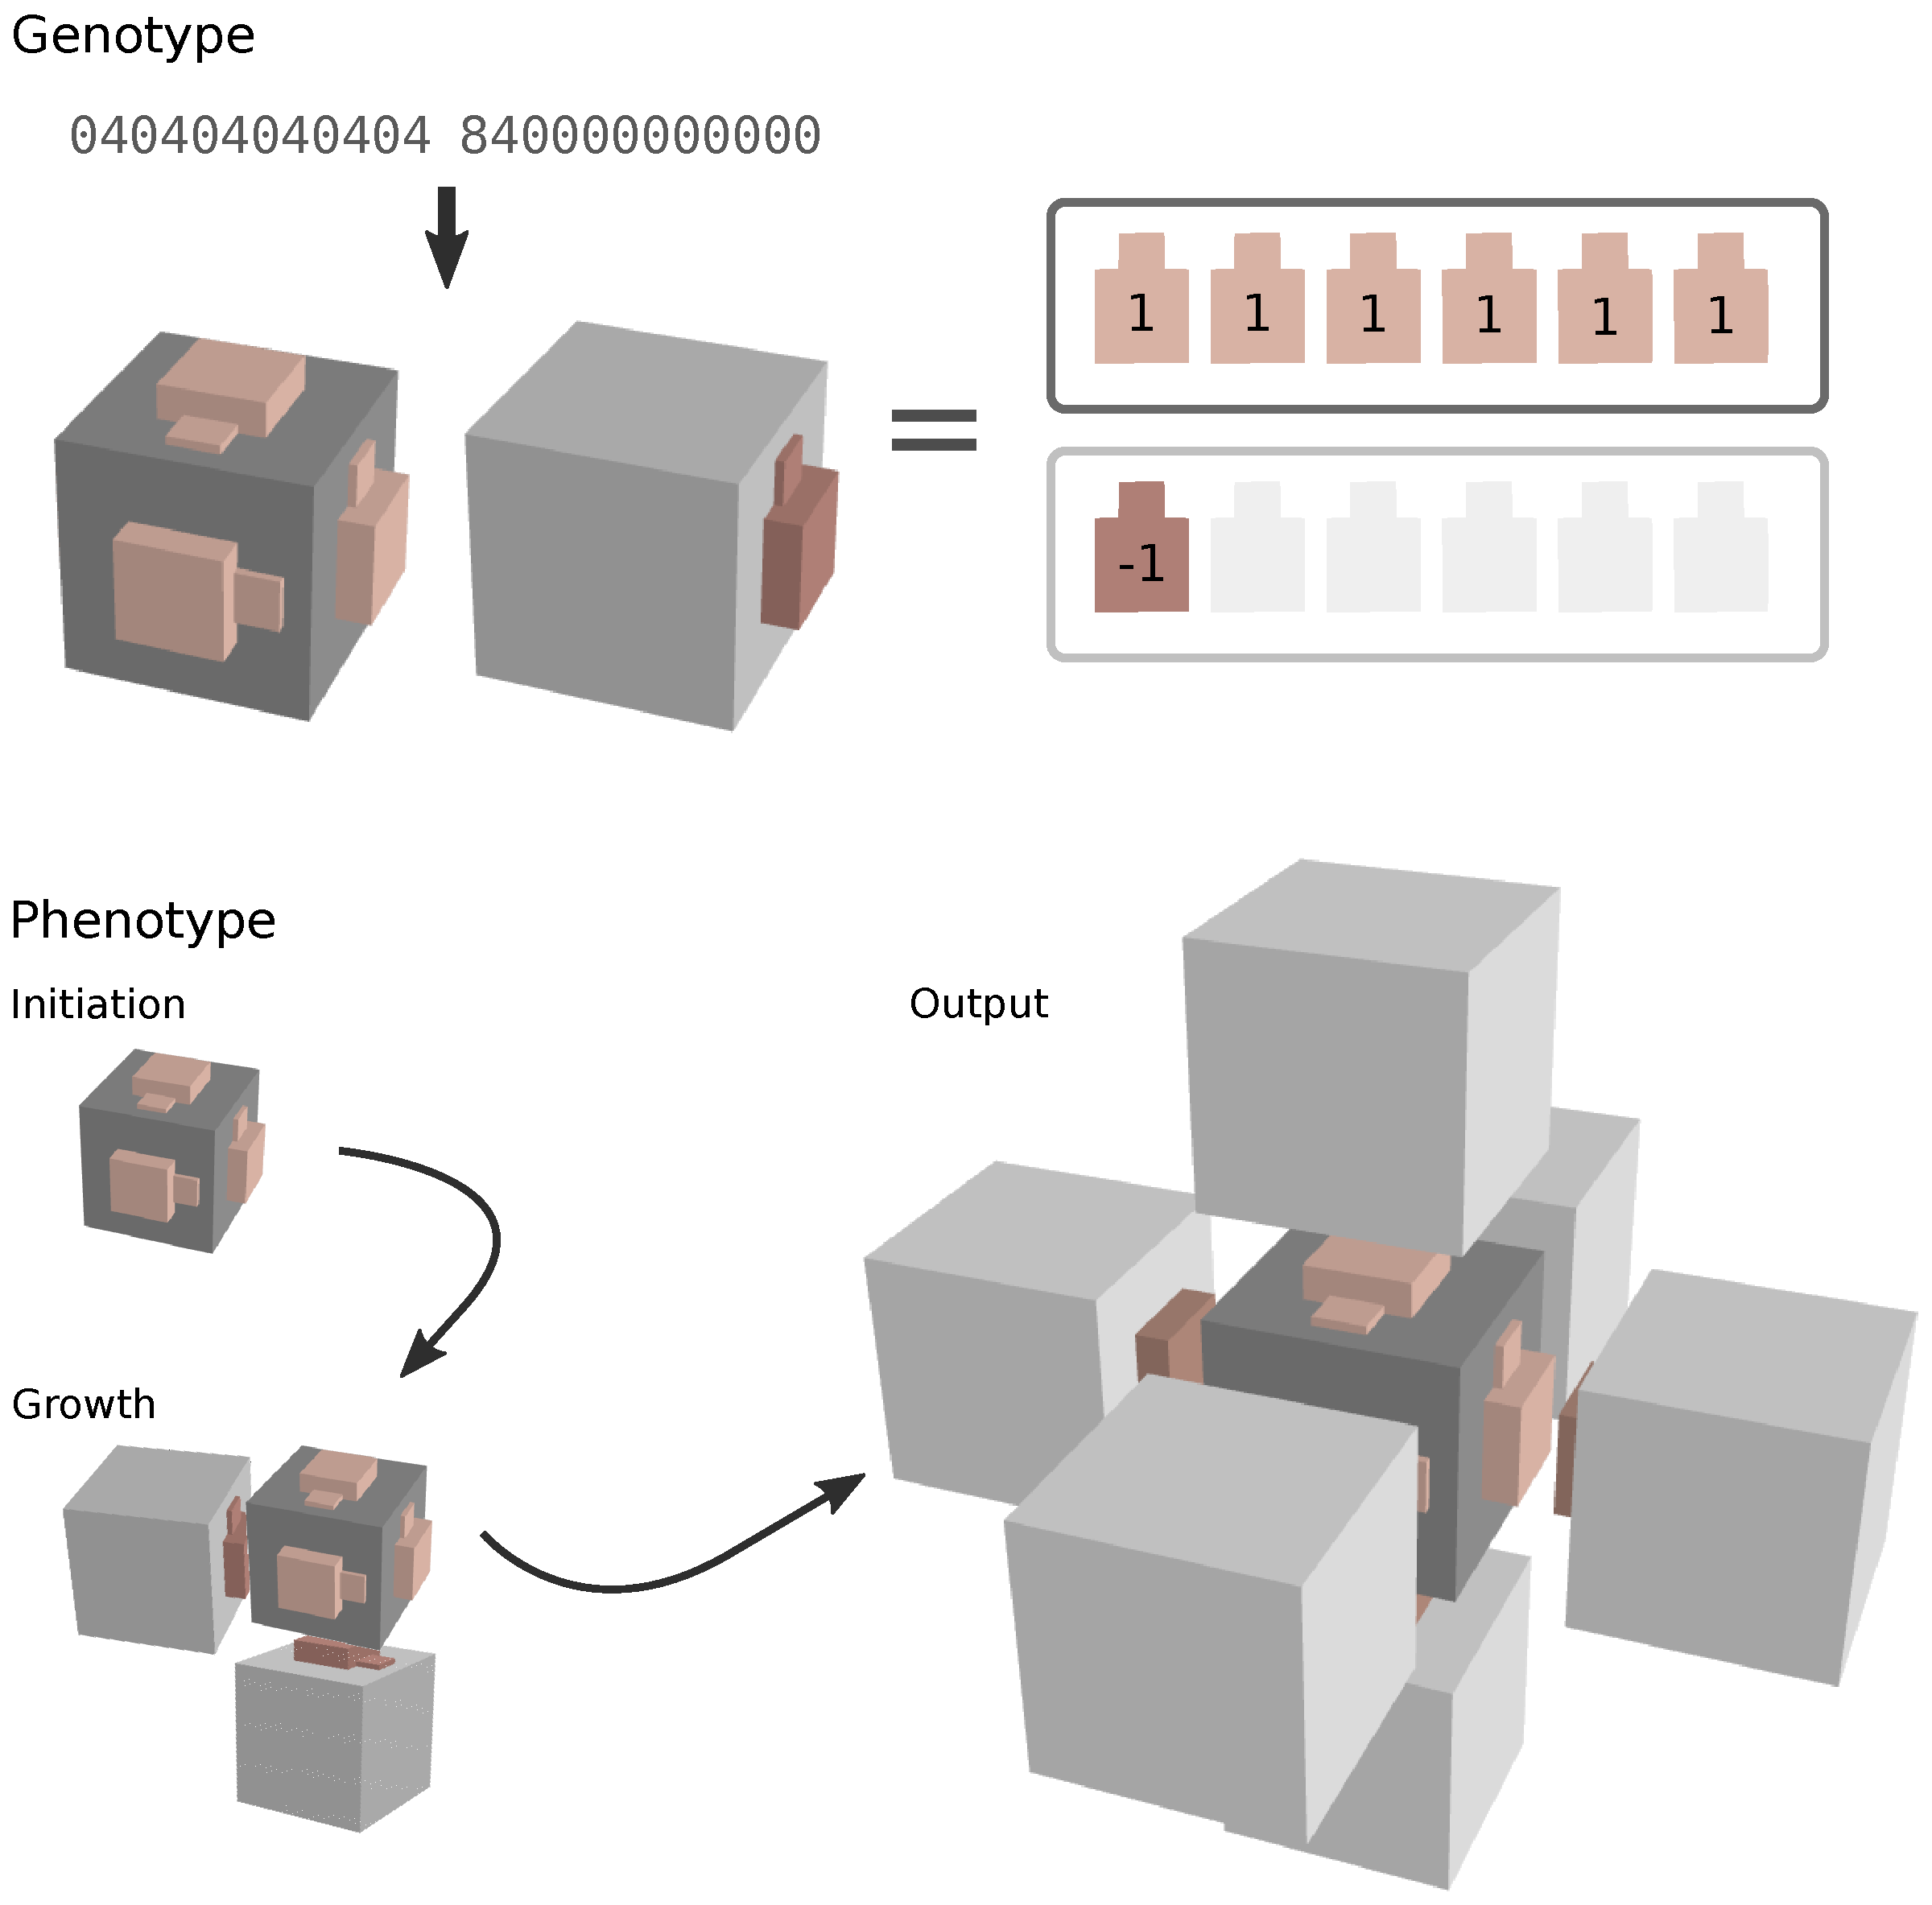
\includegraphics[width=0.8\textwidth]{figures/rule.eps} 
\caption{Illustration of the polycube assembly model. Compare to the polyomino model in Figure \ref{fig:polyominoes}. The top of the figure shows the genotype, in the form of a rule with two species one colour. The rule is visualised in three different ways. The first is a hexadecimal representations, with each two digits coding for a patch and a total of 12 digits describing a species. The second representation is of the two species shown as 3D cubes. The first species has colour=1 on all patches while the second has a single patch with colour=-1. Since the polycube is symmetric the patch rotations do not matter and are all kept at 0.}
\label{fig:polycubeRule}\end{figure}

For an illustration of the model, see Figure \ref{fig:polycubeRule}. The example in the figure is a three-dimensional "cross" structure created from a rule of size 2. The initial seeding cube belongs to the first species, enabling six additional cubes, all belonging to the second species, to bind at each patch. They bounds are made since the patch colours \(1\) and\( -1\) are opposites. After all six outer cubes have bound, there are no remaining possible moves and thus the polycube stops growing. Since the growth stops, this particular polycube is bounded, at a size of seven cubes. Furthermore, since the rule gives the same polycube every time it is evaluated, the polycube is deterministic.

\begin{figure}
    \centering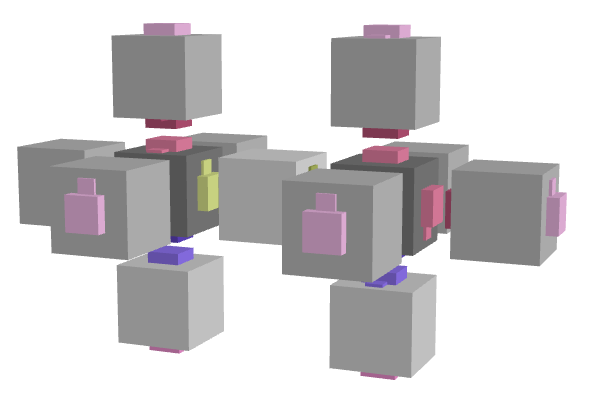
\includegraphics[align=c,width=0.24\textwidth]{figures/dnaRoboticPolycubes/doubleplus.png}\hfill
    \centering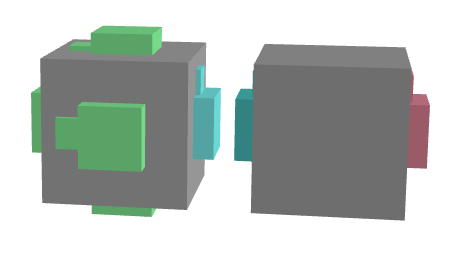
\includegraphics[align=c,width=0.24\textwidth]{figures/dnaRoboticPolycubes/swimmer.png}\hfill
    \centering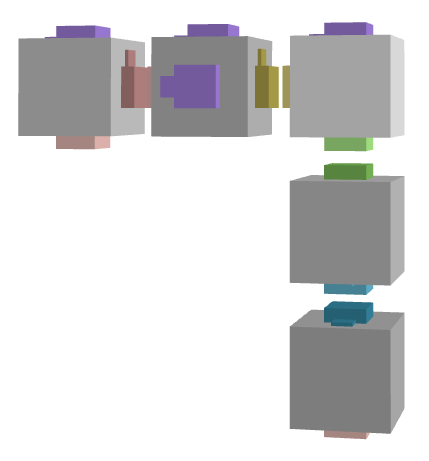
\includegraphics[align=c,width=0.24\textwidth]{figures/dnaRoboticPolycubes/L.png}\hfill
    \centering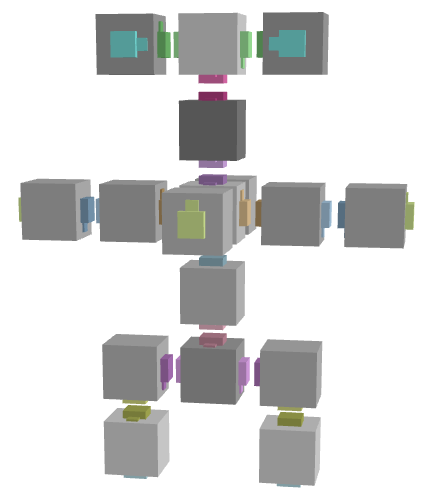
\includegraphics[align=c,width=0.24\textwidth]{figures/dnaRoboticPolycubes/robot.png}
\caption{Polycube versions of the conceptual DNA Robotics designs. Compare to Figure \ref{fig:dnaRoboticsHeader}. From left to right, the size of the rule required to specify each polyomino is: \href{https://akodiat.github.io/polycubes/view?hexRule=040890040707840c00000000888a00000000101400000000}{\underline{4}}, \href{https://akodiat.github.io/polycubes/view?hexRule=0a040b0b080a840e00000000}{\underline{2}}, \href{https://akodiat.github.io/polycubes/view?hexRule=06000c0b00001284000b080a0090140b00000000188c0000000014980000}{\underline{5}} and \href{https://akodiat.github.io/polycubes/view?hexRule=0406008800008400240000008c0800000000903400000000980c2f2f10129c1a0000000094000000002214141c000000000028a40000ac3200000000b43000000000}{\underline{11}}. Note how the third polyomino (L-shaped) requires a larger rule than the first (double cross), although it is smaller in size. This is because each cube in the L-shaped nanobot needs to be unique, while the double-cross-shaped first nanobot consists of two identical parts. If we only wished to reproduce the polycube shape, the rulesets could be minimised further.}
\label{fig:dnaRoboticPolycubes}\end{figure}

The polycube assembly model has been implemented in two versions: one browser implementation for outreach activities and accessible visualisation, and one C++ implementation for fast rule evaluation. Using the C++ implementation, large sets of random rules have been evaluated and the resulting polycubes examined and categorised. This has also been repeated for different values of rule size and colour limits.

See figure \ref{fig:rs_vs_ps} for a heat map of the frequency of rules of a certain size creating polycubes of a certain size. Notice how only three different polycube sizes were found for one species. This is understandable when inspecting the first column in Figure \ref{fig:poly_examples}; using only one species, you cannot create a bounded structure of any other size.

For larger rule sizes, polycubes can have any form, as shown in Figure \ref{fig:dnaRoboticPolycubes}, but upon inspection of the larger polycube sizes (and small rule sizes) from Figure \ref{fig:rs_vs_ps}, the polycubes all seem to be highly symmetrical, as shown in \ref{fig:poly_examples}.
%I have already implemented a fast version of the code that can generate random rules with a certain max amount of "colours" and tile types. The next step is to determine what (deterministic) structures are more common. (Rules creating non-deterministic structures are disregarded, but their percentage of the total is still noted). Plotting the probability of each structure, from a random rule, against a measure of its complexity, do we get a power-law distribution (as in Iain Johnston's polyomino paper)?


\begin{figure}
\centering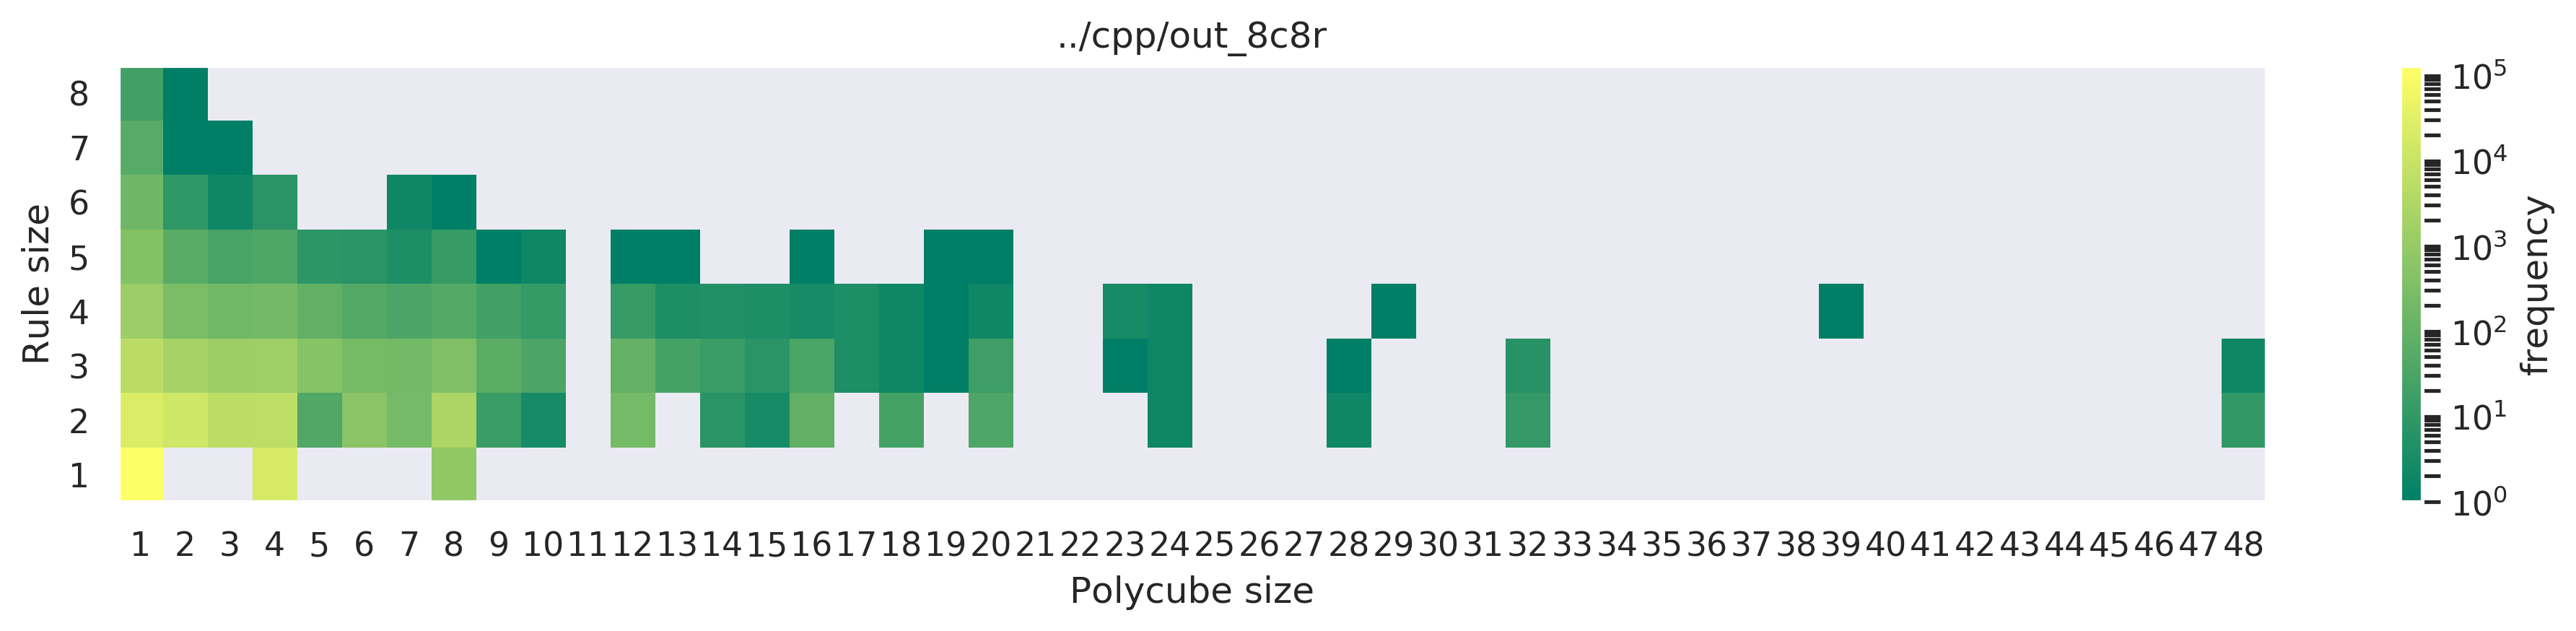
\includegraphics[width=\textwidth]{figures/rs_vs_ps_8c8r.png}
\caption{Heat map of rule size vs polycube size, for a simulation with a maximum of 8 species and a limit of 8 colours, evaluating 2.5 million random rules. Note that the frequency scale is logarithmic.}
\label{fig:rs_vs_ps}\end{figure}

\begin{figure}
%\centering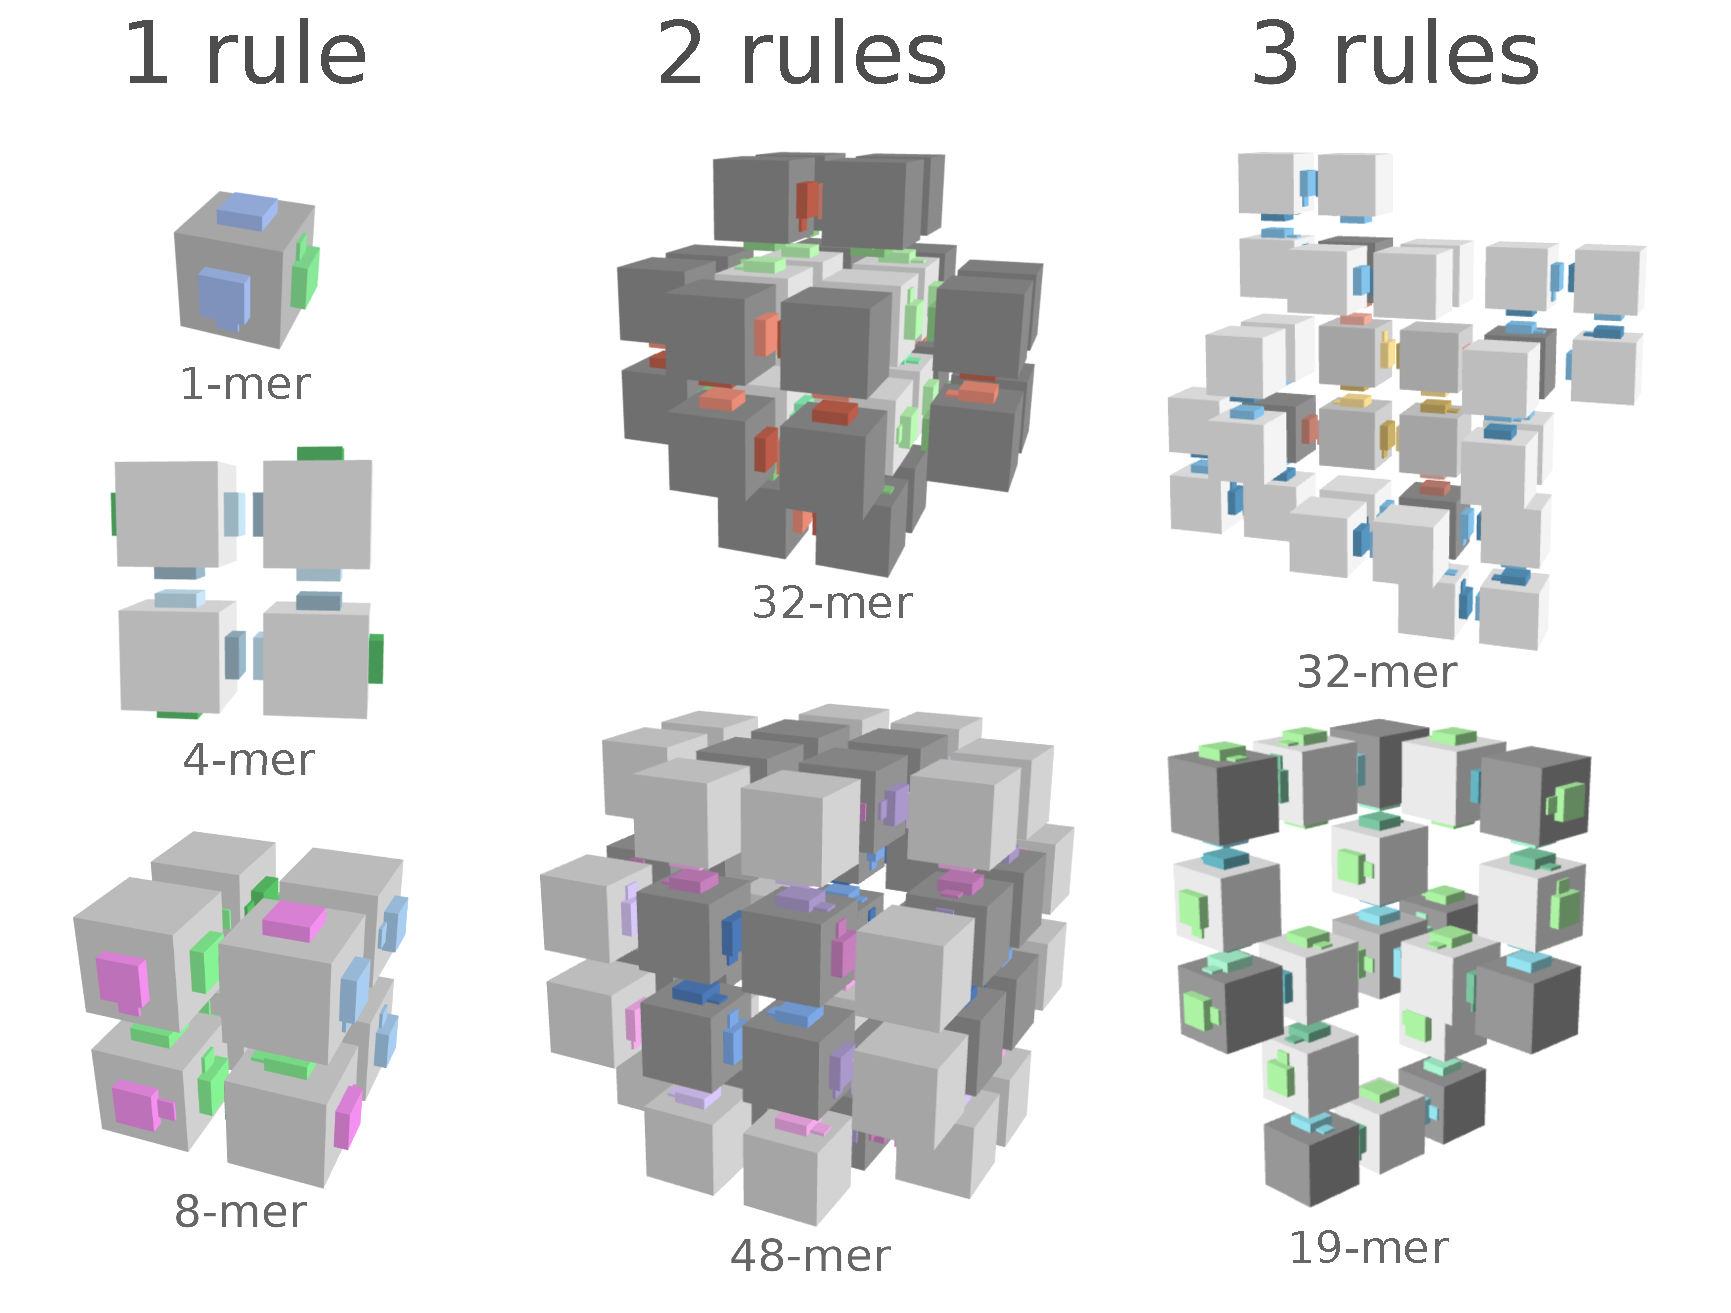
\includegraphics[width=\textwidth]{figures/examples.eps}
\caption{Example of polycubes grown from 1, 2 and 3 speciess. Although any polycube can be encoded into a rule, the larger polycubes that have small rules tend to be symmetrical. This agrees with Johnston's polyomino model in that they have low complexity}
\label{fig:poly_examples}\end{figure}

\section{Sampling the space of assembly rules}

\[
I_{n_c, n_t} = (4(1+2n_c))^{6n_t}
\]

Trying all inputs in a brute-force approach is impossible. Even if we limit both the amount of allowed colours \(n_c\) and the amount of species \(n_t\) to eight, the space of possible inputs, with four patch orientations and six patches per cube, is \(I_{8, 8} \approx 9*10^{87}\).
But, while this is too large to sample fully, we can still get an idea of how likely it is for an input to map to a certain output by taking samples of the space of possible input rules.

This was done by uniformly sampling and assembling one billion random rules from \(I_{8, 8}\). Rules growing larger than 100 cubes were discarded as unbounded, while those remaining bounded were re-assembled 15 times to ensure they assembled deterministically. Deterministic and bounded output was then grouped by their shapes, counting the number of times each given phenotype occurs. For each rule found to produce a given phenotype, the number of colours is multiplied with the number of species in the rule, producing a measure of the rule size. The smallest such rule size is then used as a proxy for the phenotype complexity.

\section{Complexity bias}

As can be seen in Figure \ref{fig:plot}, there is a clear log-linear relationship between the probability of finding a rule that assembles into a particular structure, and the information needed to specify the structure, as predicted in \cite{dingle2018input, dingle2020generic}.

\section{Robustness}

\chapter{\label{ch:polycubes2}Designing polycube assembly rules}

\minitoc

In the previous chapter, we used random input rules to explore properties of the corresponding distributions of output polycube shapes. However, the reverse problem is just as significant; given a target shape, how do you find a rule that assembles it?  

% Fully addressable is the easy solution.

A trivial solution would be to use \emph{fully addressable assembly}: simply assign a unique species to each cube and a unique colour to each pair of adjacent patches. This is similar to the design principle underlying DNA bricks (Section~\ref{sec:dna_tiles_bricks}), where every brick tile is unique. However, as was seen in Chapter~\ref{ch:polycubes1}, many shapes have alternative solutions requiring widely different numbers of unique components. See Figure~\ref{fig:addressable}, where a square tetromino is shown to have a variety of inputs assembling it, from the minimal solution with just a single species and one colour, up to the fully addressable solution with four species and four colours (\(\widetilde{K}_s = \widetilde{K}_c = 4\)). The intermediate solutions are not necessarily deterministic in terms of which position gets which species, but they will always assemble into the same shape.

% Andrew: Explain the significance of mismatched colours.

Meanwhile, the empty red region in Figure~\ref{fig:addressable}.b) shows combinations of \(\widetilde{K}_s\) and \(\widetilde{K}_c\) for which a solution is not possible. For example, if you use a single species, you cannot use more than one colour.

\begin{figure}[ht]
    \centering
    \begin{overpic}[width=\textwidth]{figures/solve/adressable.eps}
        \put(-10,480){a)}
        \put(360,580){b)}

        \put(370, 350){\makebox(0,0){\rotatebox{90}{Number of colours (\(\widetilde{K}_c\))}}}
        \put(600,-30){Number of species (\(\widetilde{K}_s\))}
    \end{overpic}
    \vspace{1em}
    %\includesvg[width=\textwidth, inkscapelatex=false]{figures/solve/adressable.svg}
    \caption{\(2 \times 2\) square polyomino assembled with different levels of complexity. \textbf{a)} Schematic of the input shape, consisting of four connected tiles. \textbf{b)} The green region shows possible assembly solutions, from the \emph{minimal solution} using a single species and a single colour (bottom left), to the \emph{fully addressable solution} using four species and colours (top right). The red region lacks solutions. }
    \label{fig:addressable}
\end{figure}

So, how do we find alternative and simpler input rules for a shape? Surely, there must exist a better method than sampling the space of all rules (as done in Chapter~\ref{ch:polycubes1})? This chapter presents an approach where \emph{satisfiability solving} is used to determine if a shape can be assembled from a given number of colours and species, thus automatically filling in solution landscapes such as the one shown in Figure~\ref{fig:addressable}. A complementary approach substituting similar species is also described in Section~\ref{sec:substitution_solving}.


\section{Satisfiability solving}

Building upon a published method for determining patchy particle interactions for unbounded structures \cite{romano2020designing}, it is possible to formulate and solve satisfiability problems that map onto assembly rules for the bounded polycube structures.

In essence, we formulate a boolean expression that, if true, means it is possible to assemble a given polycube topology using a given number of colours and species. We can then use a satisfiability solver to check if that expression is indeed solvable and, if it is, extract an assembly rule from the solution.

\subsection{Boolean expressions}

The boolean expression is written in conjunctive normal form (CNF), where variables are composed into clauses using \emph{NOT} (\(\lnot\)) and \emph{OR} (\(\lor\)) operators and where the clauses are joined by \emph{AND} (\(\land\)) operators. As a simple example, see the expression below:

\[
    (\lnot x_{rain} \lor x_{umbrella} \lor  \lnot x_{walk}) \land
    (\lnot x_{rainbow} \lor x_{rain}) \land
    (\lnot x_{rainbow} \lor x_{sunny})
\]

The first clause is \({true}\) for all values except when \(x_{rain}={true}\), \(x_{umbrella}={false}\) and \(x_{walk}=true\); so the solution of taking a walk in the rain without an umbrella is forbidden. This could also be written as an \emph{implication}: \(x_{rain} \land x_{walk} \implies x_{umbrella}\).

The following two clauses in the example above are the CNF form of another implication: \(x_{rainbow} \implies  x_{rain} \land x_{sunshine}\), stating that a rainbow implies that we have both rain and sunshine (we cannot have a rainbow without rain or without sunshine). The full expression is satisfiable, for example, if we set \(x_{sun}=true\), \(x_{rain}=false\), \(x_{walk}=false\), \(x_{umbrella}=false\), and \(x_{rainbow}=false\); ignoring the walk in the sunshine and remaining inside to work.

\subsection{Polycube formulation}

For the polycube problem, we introduce the following variables:
\begin{description}
    \item[\(x_{l,p,o}^{A}\)] (patch \(p\) at position \(l\) has orientation \(o\))
    \item[\(x_{c_i,c_j}^{B}\)] (colour \(c_i\) is compatible with colour \(c_j\))
    \item[\(x_{s,p,c}^{C}\)] (patch \(p\) on species \(s\) has colour \(c\))
    \item[\(x_{p_1,o_1,p_2,o_2}^{D}\)] (patch \(p_1\) with orientation \(o_1\) binds to patch \(p_2\) with orientation \(o_2\))
    \item[\(x_{l,p,c}^{F}\)] (patch \(p\) at position \(l\) has colour \(c\))
    \item[\(x_{s,p,o}^{O}\)] (patch \(p\) on species \(s\) has orientation \(o\))
    \item[\(x_{l,s,r}^{P}\)] (position \(l\) is occupied by species \(s\) rotated by \(r\))] 
\end{description}

We then formulate clauses to constrain the problem, seen in Table~\ref{tab:sat_clauses}. Clauses (i)-(vii) are the same as in \cite{romano2020designing} while the remaining are added, together with variables \(x^D\), \(x^A\) and \(x^O\) above, to include \emph{torsional restrictions}, meaning that patches need to bind at a compatible orientation (compared to being allowed to rotate freely).

\begin{table}[h!]
    \centering
    \begin{tabular}{|l|l|l|}
        \hline
        & Clause & Boolean expression \\ [0.5ex] 
        \hline
        \hline
        (i) & \(C^{B}_{c_i,c_j,c_k}\) & \(\neg x_{c_i,c_j}^{B} \lor \neg x_{c_i,c_k}^{B}\) \\ % Each colour is compatible with exactly one colour
        (ii) &  \(C^{C}_{s,p,c_k,c_l}\) & \(\neg x_{s, p, c_k}^{C} \lor \neg x_{s, p, c_l}^{C}\) \\ % Each patch is assigned exactly one colour
        (iii) & \(C^{P}_{l, s_i, r_i, s_j, r_j}\)  & \(\neg x_{l,s_i,r_i}^{P} \lor \neg x_{l,s_j,r_j}^{P} \) \\ % Each lattice position is occupied by a single species with one assigned rotation
        (iv) & \(C^{BF}_{l_i,p_i,c_i,l_j,p_j,c_j}\) & \(\left(x_{l_i,p_i,c_i}^{F} \land x_{l_j,p_j,c_j}^{F} \right) \Rightarrow x_{c_i,c_j}^{B}\) \\ % Colours of patches that interact in the target lattice must be compatible
        (v) & \(C^{rotC}_{l,s,r,p,c}\) & \(x_{l,s,r}^{P} \Rightarrow \left(x_{l,p,c}^{F} \Leftrightarrow x_{s, \phi_r(p), c}^{C}\right)\) \\ % The patches at a lattice position is set to have the patch colours of the rotated occupying species.
        (vi) & \(C^{all s}_{s}\)  & \(\bigvee_{\forall l, r} x_{l,s,r}^{P}\) \\ % All \widetilde{K}_s species are used for the lattice assembly
        (vii) & \(C^{all c}_{c}\)  & \(\bigvee_{\forall s, p} x_{s,p,c}^{C}\) \\ % All \widetilde{K}_c patch colours are used in the solution
        (iix) &  \(C^{O}_{s,p,o_k,o_l}\) & \(\neg x_{s, p, o_k}^{O} \lor \neg x_{s, p, o_l}^{O}\) \\ % Each patch is assigned exactly one orientation
        (ix) & \(C^{DA}_{l_i,p_i,c_i,l_j,p_j,c_j}\) & \(\left(x_{l_i,p_i,c_i}^{A} \land x_{l_j,p_j,c_j}^{A} \right) \Rightarrow x_{p_i,c_i,p_j,c_j}^{D}\) \\ % Orientation of patches that interact in the target lattice must be compatible
        (x) & \(C^{rotO}_{l,s,r,p,o}\) & \(x_{l,s,r}^{P} \Rightarrow \left(x_{l,p,o}^{A} \Leftrightarrow x_{s, \phi_r(p), o}^{O}\right)\) \\ % The patches at a lattice position is set to have the orientations of the rotated occupying species.
        \hline
    \end{tabular}
    \caption{SAT clauses. (i) Each colour is compatible with \textit{exactly one} colour. (ii) Each patch has \textit{exactly one} colour. (iii) Each lattice position contains a single species with an assigned rotation. (iv) Adjacent patches in the lattice must have compatible colours. (v) Patches at a lattice position are coloured according to the (rotated) occupying species. (vi) All \(\widetilde{K}_s\) species are required in the solution. (vii) All \(\widetilde{K}_c\) patch colours are required in the solution. (iix) Each patch is assigned \textit{exactly one} orientation. (ix) Adjacent patches in the target lattice must have the same orientation. (v)  Patches at a lattice position are oriented according to the (rotated) occupying species.}
    \label{tab:sat_clauses}

    % Andrew: I would make a full-page table with the English statement as an additional column.
    \end{table}

\subsection{On the importance of torsional interactions}

It would certainly be possible to use the solver without any constraints on the patch orientations (as it was done in \cite{romano2020designing}). However, if we wanted to use the stochastic assembler from Chapter~\ref{ch:polycubes1}, orientations would have to be assigned randomly, resulting in a combinatoric explosion of additional assembly paths.

More importantly, the assembly should benefit from torsional patch interaction (for 2D polyominoes, this corresponds to the requirement that tiles can be rotated in the plane but not flipped). Figure~\ref{fig:torsion} shows two versions of a simple rule, the only difference being the orientation of a single patch. While co-operative binding might, in such a case, benefit the desired square assembly, the self-limiting ability would be significantly improved if the patches were torsionally rigid.

\begin{figure}[ht]
    \centering
    \begin{overpic}[width=\textwidth]{figures/torsion.png}
        \put(0,470){a)}
        \put(550,500){b)}
    \end{overpic}
    \caption{The consequences of a rotated patch. \textbf{a)} A minimal solution (one species and one colour) for a \(2 \times 2\) square. \textbf{b)} The same rule as a), except one patch on is rotated by \(\frac{\pi}{2}\).}
    \label{fig:torsion}
\end{figure}


\subsection{Bounded structures}
Besides the torsional patches, another important difference to \cite{romano2020designing} is that the method presented here allows for bounded structures. This is achieved by adding species of type ``empty'' as a "shell" around the shape to ensure that empty patches remain unbound. Adding a clause \(x_{0,1}^{B}\) ensures that colour 0 (on the shell) always binds to 1 (on the boundary). 

We then add clauses \(x_{l,p,1}^{F}\) to constrain every boundary patch \(p\) at lattice position \(l\) to have the colour \(1\) and thereby not bind anything else. For example, in Figure~\ref{fig:sat_boundary}, where these boundary patches are seen coloured white (and bordering an empty square), we get the following 12 clauses:

\begin{equation}
    \begin{aligned}
        &x_{0,0,1}^{F} \land x_{0,1,1}^{F} \land x_{0,3,1}^{F} \land \\
        &x_{1,0,1}^{F} \land x_{1,2,1}^{F} \land x_{1,3,1}^{F} \land \\
        &x_{3,0,1}^{F} \land x_{3,1,1}^{F} \land x_{3,2,1}^{F} \land \\
        &x_{4,1,1}^{F} \land x_{4,2,1}^{F} \land x_{4,3,1}^{F}
    \end{aligned}
\end{equation}

Note that for 3D polycubes, there are six patches per species instead of the four seen in the 2D polyomino in Figure~\ref{fig:sat_boundary}. This also introduces 27 possible cube rotations, compared to the 4 square rotations defined for 2D.

The topology of the shape is enforced by clause (iv), \(\left(\lnot x_{l_1, p_1, c_1}^{F} \lor \lnot x_{l_2, p_2, c_2}^{F} \lor x_{c_1, c_2}^{B}\right)\) in CNF, making sure that if patch \(p_1\) on lattice position \(l_1\) binds to \(p_2\) on lattice position \(l_2\), their colours are compatible. Similarly, clause (ix) ensures that the patches have the same orientation.

% Figure of topology graph?

\begin{figure}[ht]
    \centering\includesvg[width=.5\textwidth, inkscapelatex=false]{figures/sat_boundary.svg}
    \caption{Bounded shape topology for satisfiability solving. Patches at the boundary of the shape (white) are constrained to only bind to ``empty''. 3D shapes are specified the same way, but with six patches per species.}
    \label{fig:sat_boundary}
\end{figure}

\subsection{Interaction matrix}
Compared to \cite{romano2020designing}, the interaction matrix is by default fixed. Thus, the \(x_{c_i,c_j}^{B}\) variable has fixed values and we only need to extract the values of \(x_{l,p,c}^{F}\) and \(x_{s,p,o}^{O}\) to construct the assembly rule. Note, however, that it is still possible to re-enable a variable interaction matrix, something which could prove useful for some shapes where, for example, self-complementary patches would result in a lower complexity.

Compared to the interaction matrix convention used in Chapter~\ref{ch:polycubes1}, where each colour \(c\) binds to \(-c\), the colour values in the SAT solver remain unsigned and instead pair each even colour \(c\) to the odd \(c+1\). The colour pairs are mapped back to the polycube convention when obtaining the solution.

\subsection{Assembly determinism}
Even if the SAT solver determines that a solution exists, it is still possible that the rule we get can also assemble into other shapes. Recall, once more, the ``giraffe duck'' shape from Figure~\ref{fig:UND}.b). If we solved for the shape with two neck cubes, the non-deterministic rule shown would be a perfectly valid solution according to the SAT solver, even though it can also produce giraffe ducks with any other neck length.

Because of this, we once again use the stochastic assembler to verify that the rule assembles into the correct shape every time. Each potential rule is evaluated a large number of times (by default \(100\)), calculating an assembly ratio. If the ratio is \(1\), the rule is considered bounded and deterministic and, as such, a valid solution.


\section{Finding the minimal assembly rule}

By iteratively ruling out lower values of \(\widetilde{K}_s\) and \(\widetilde{K}_c\), a minimal solution can be found, as detailed in Figure~\ref{fig:sat_alg}. It is also possible to generate and compare alternative solutions of varying complexity. While forbidding an undefined solution and retrying could in principle, continue until the computer runs out of memory (or the solution is disproven or valid), the results presented below used a limit of 100 retries before moving on.

The exploration of the solution landscape can also be done in parallel, with each combination of \(\widetilde{K}_s\) and \(\widetilde{K}_c\) explored concurrently.

\begin{figure}
    \centering
    \resizebox{\textwidth}{!}{% Graphic for TeX using PGF
% Title: /home/joakim/Documents/polycube/SAT_flow.dia
% Creator: Dia v0.97+git
% CreationDate: Thu May 27 10:43:08 2021
% For: joakim
% \usepackage{tikz}
% The following commands are not supported in PSTricks at present
% We define them conditionally, so when they are implemented,
% this pgf file will use them.
\ifx\du\undefined
  \newlength{\du}
\fi
\setlength{\du}{15\unitlength}
\begin{tikzpicture}[even odd rule]
\pgftransformxscale{1.000000}
\pgftransformyscale{-1.000000}
\definecolor{dialinecolor}{rgb}{0.000000, 0.000000, 0.000000}
\pgfsetstrokecolor{dialinecolor}
\pgfsetstrokeopacity{1.000000}
\definecolor{diafillcolor}{rgb}{1.000000, 1.000000, 1.000000}
\pgfsetfillcolor{diafillcolor}
\pgfsetfillopacity{1.000000}
\pgfsetlinewidth{0.100000\du}
\pgfsetdash{}{0pt}
\pgfsetmiterjoin
{\pgfsetcornersarced{\pgfpoint{0.000000\du}{0.000000\du}}\definecolor{diafillcolor}{rgb}{1.000000, 1.000000, 1.000000}
\pgfsetfillcolor{diafillcolor}
\pgfsetfillopacity{1.000000}
\fill (13.087793\du,24.536630\du)--(13.087793\du,26.436630\du)--(19.140293\du,26.436630\du)--(19.140293\du,24.536630\du)--cycle;
}{\pgfsetcornersarced{\pgfpoint{0.000000\du}{0.000000\du}}\definecolor{dialinecolor}{rgb}{0.000000, 0.000000, 0.000000}
\pgfsetstrokecolor{dialinecolor}
\pgfsetstrokeopacity{1.000000}
\draw (13.087793\du,24.536630\du)--(13.087793\du,26.436630\du)--(19.140293\du,26.436630\du)--(19.140293\du,24.536630\du)--cycle;
}% setfont left to latex
\definecolor{dialinecolor}{rgb}{0.000000, 0.000000, 0.000000}
\pgfsetstrokecolor{dialinecolor}
\pgfsetstrokeopacity{1.000000}
\definecolor{diafillcolor}{rgb}{0.000000, 0.000000, 0.000000}
\pgfsetfillcolor{diafillcolor}
\pgfsetfillopacity{1.000000}
\node[anchor=base,inner sep=0pt, outer sep=0pt,color=dialinecolor] at (16.114043\du,25.681630\du){Try \(N_c\) and \(N_t\)};
% setfont left to latex
\definecolor{dialinecolor}{rgb}{0.000000, 0.000000, 0.000000}
\pgfsetstrokecolor{dialinecolor}
\pgfsetstrokeopacity{1.000000}
\definecolor{diafillcolor}{rgb}{0.000000, 0.000000, 0.000000}
\pgfsetfillcolor{diafillcolor}
\pgfsetfillopacity{1.000000}
\node[anchor=base west,inner sep=0pt,outer sep=0pt,color=dialinecolor] at (27.290293\du,24.956775\du){Yes};
% setfont left to latex
\definecolor{dialinecolor}{rgb}{0.000000, 0.000000, 0.000000}
\pgfsetstrokecolor{dialinecolor}
\pgfsetstrokeopacity{1.000000}
\definecolor{diafillcolor}{rgb}{0.000000, 0.000000, 0.000000}
\pgfsetfillcolor{diafillcolor}
\pgfsetfillopacity{1.000000}
\node[anchor=base west,inner sep=0pt,outer sep=0pt,color=dialinecolor] at (24.240293\du,28.331775\du){No};
\pgfsetlinewidth{0.100000\du}
\pgfsetdash{}{0pt}
\pgfsetmiterjoin
{\pgfsetcornersarced{\pgfpoint{0.000000\du}{0.000000\du}}\definecolor{diafillcolor}{rgb}{1.000000, 1.000000, 1.000000}
\pgfsetfillcolor{diafillcolor}
\pgfsetfillopacity{1.000000}
\fill (39.101543\du,24.536630\du)--(39.101543\du,26.436630\du)--(42.064043\du,26.436630\du)--(42.064043\du,24.536630\du)--cycle;
}{\pgfsetcornersarced{\pgfpoint{0.000000\du}{0.000000\du}}\definecolor{dialinecolor}{rgb}{0.000000, 0.000000, 0.000000}
\pgfsetstrokecolor{dialinecolor}
\pgfsetstrokeopacity{1.000000}
\draw (39.101543\du,24.536630\du)--(39.101543\du,26.436630\du)--(42.064043\du,26.436630\du)--(42.064043\du,24.536630\du)--cycle;
}% setfont left to latex
\definecolor{dialinecolor}{rgb}{0.000000, 0.000000, 0.000000}
\pgfsetstrokecolor{dialinecolor}
\pgfsetstrokeopacity{1.000000}
\definecolor{diafillcolor}{rgb}{0.000000, 0.000000, 0.000000}
\pgfsetfillcolor{diafillcolor}
\pgfsetfillopacity{1.000000}
\node[anchor=base,inner sep=0pt, outer sep=0pt,color=dialinecolor] at (40.582793\du,25.681630\du){Done};
% setfont left to latex
\definecolor{dialinecolor}{rgb}{0.000000, 0.000000, 0.000000}
\pgfsetstrokecolor{dialinecolor}
\pgfsetstrokeopacity{1.000000}
\definecolor{diafillcolor}{rgb}{0.000000, 0.000000, 0.000000}
\pgfsetfillcolor{diafillcolor}
\pgfsetfillopacity{1.000000}
\node[anchor=base west,inner sep=0pt,outer sep=0pt,color=dialinecolor] at (37.640293\du,24.756775\du){Yes};
% setfont left to latex
\definecolor{dialinecolor}{rgb}{0.000000, 0.000000, 0.000000}
\pgfsetstrokecolor{dialinecolor}
\pgfsetstrokeopacity{1.000000}
\definecolor{diafillcolor}{rgb}{0.000000, 0.000000, 0.000000}
\pgfsetfillcolor{diafillcolor}
\pgfsetfillopacity{1.000000}
\node[anchor=base west,inner sep=0pt,outer sep=0pt,color=dialinecolor] at (33.890293\du,29.156775\du){No};
\pgfsetlinewidth{0.100000\du}
\pgfsetdash{}{0pt}
\pgfsetmiterjoin
\definecolor{diafillcolor}{rgb}{1.000000, 1.000000, 1.000000}
\pgfsetfillcolor{diafillcolor}
\pgfsetfillopacity{1.000000}
\fill (23.943082\du,23.300000\du)--(27.486164\du,25.486630\du)--(23.943082\du,27.673261\du)--(20.400000\du,25.486630\du)--cycle;
\definecolor{dialinecolor}{rgb}{0.000000, 0.000000, 0.000000}
\pgfsetstrokecolor{dialinecolor}
\pgfsetstrokeopacity{1.000000}
\draw (23.943082\du,23.300000\du)--(27.486164\du,25.486630\du)--(23.943082\du,27.673261\du)--(20.400000\du,25.486630\du)--cycle;
% setfont left to latex
\definecolor{dialinecolor}{rgb}{0.000000, 0.000000, 0.000000}
\pgfsetstrokecolor{dialinecolor}
\pgfsetstrokeopacity{1.000000}
\definecolor{diafillcolor}{rgb}{0.000000, 0.000000, 0.000000}
\pgfsetfillcolor{diafillcolor}
\pgfsetfillopacity{1.000000}
\node[anchor=base,inner sep=0pt, outer sep=0pt,color=dialinecolor] at (23.943082\du,25.681630\du){Satisfiable?};
\pgfsetlinewidth{0.100000\du}
\pgfsetdash{}{0pt}
\pgfsetmiterjoin
\definecolor{diafillcolor}{rgb}{1.000000, 1.000000, 1.000000}
\pgfsetfillcolor{diafillcolor}
\pgfsetfillopacity{1.000000}
\fill (33.444978\du,22.430375\du)--(37.941584\du,25.486630\du)--(33.444978\du,28.542886\du)--(28.948372\du,25.486630\du)--cycle;
\definecolor{dialinecolor}{rgb}{0.000000, 0.000000, 0.000000}
\pgfsetstrokecolor{dialinecolor}
\pgfsetstrokeopacity{1.000000}
\draw (33.444978\du,22.430375\du)--(37.941584\du,25.486630\du)--(33.444978\du,28.542886\du)--(28.948372\du,25.486630\du)--cycle;
% setfont left to latex
\definecolor{dialinecolor}{rgb}{0.000000, 0.000000, 0.000000}
\pgfsetstrokecolor{dialinecolor}
\pgfsetstrokeopacity{1.000000}
\definecolor{diafillcolor}{rgb}{0.000000, 0.000000, 0.000000}
\pgfsetfillcolor{diafillcolor}
\pgfsetfillopacity{1.000000}
\node[anchor=base,inner sep=0pt, outer sep=0pt,color=dialinecolor] at (33.444978\du,25.281630\du){Bounded \&};
% setfont left to latex
\definecolor{dialinecolor}{rgb}{0.000000, 0.000000, 0.000000}
\pgfsetstrokecolor{dialinecolor}
\pgfsetstrokeopacity{1.000000}
\definecolor{diafillcolor}{rgb}{0.000000, 0.000000, 0.000000}
\pgfsetfillcolor{diafillcolor}
\pgfsetfillopacity{1.000000}
\node[anchor=base,inner sep=0pt, outer sep=0pt,color=dialinecolor] at (33.444978\du,26.081630\du){Deterministic?};
\pgfsetlinewidth{0.100000\du}
\pgfsetdash{}{0pt}
\pgfsetmiterjoin
{\pgfsetcornersarced{\pgfpoint{0.000000\du}{0.000000\du}}\definecolor{diafillcolor}{rgb}{1.000000, 1.000000, 1.000000}
\pgfsetfillcolor{diafillcolor}
\pgfsetfillopacity{1.000000}
\fill (30.669978\du,29.741575\du)--(30.669978\du,32.441575\du)--(36.272478\du,32.441575\du)--(36.272478\du,29.741575\du)--cycle;
}{\pgfsetcornersarced{\pgfpoint{0.000000\du}{0.000000\du}}\definecolor{dialinecolor}{rgb}{0.000000, 0.000000, 0.000000}
\pgfsetstrokecolor{dialinecolor}
\pgfsetstrokeopacity{1.000000}
\draw (30.669978\du,29.741575\du)--(30.669978\du,32.441575\du)--(36.272478\du,32.441575\du)--(36.272478\du,29.741575\du)--cycle;
}% setfont left to latex
\definecolor{dialinecolor}{rgb}{0.000000, 0.000000, 0.000000}
\pgfsetstrokecolor{dialinecolor}
\pgfsetstrokeopacity{1.000000}
\definecolor{diafillcolor}{rgb}{0.000000, 0.000000, 0.000000}
\pgfsetfillcolor{diafillcolor}
\pgfsetfillopacity{1.000000}
\node[anchor=base,inner sep=0pt, outer sep=0pt,color=dialinecolor] at (33.471228\du,30.886575\du){Forbid current};
% setfont left to latex
\definecolor{dialinecolor}{rgb}{0.000000, 0.000000, 0.000000}
\pgfsetstrokecolor{dialinecolor}
\pgfsetstrokeopacity{1.000000}
\definecolor{diafillcolor}{rgb}{0.000000, 0.000000, 0.000000}
\pgfsetfillcolor{diafillcolor}
\pgfsetfillopacity{1.000000}
\node[anchor=base,inner sep=0pt, outer sep=0pt,color=dialinecolor] at (33.471228\du,31.686575\du){solution};
\pgfsetlinewidth{0.100000\du}
\pgfsetdash{}{0pt}
\pgfsetbuttcap
{
\definecolor{diafillcolor}{rgb}{0.000000, 0.000000, 0.000000}
\pgfsetfillcolor{diafillcolor}
\pgfsetfillopacity{1.000000}
% was here!!!
\pgfsetarrowsend{stealth}
\definecolor{dialinecolor}{rgb}{0.000000, 0.000000, 0.000000}
\pgfsetstrokecolor{dialinecolor}
\pgfsetstrokeopacity{1.000000}
\draw (19.188296\du,25.486630\du)--(20.400000\du,25.486630\du);
}
\pgfsetlinewidth{0.100000\du}
\pgfsetdash{}{0pt}
\pgfsetbuttcap
{
\definecolor{diafillcolor}{rgb}{0.000000, 0.000000, 0.000000}
\pgfsetfillcolor{diafillcolor}
\pgfsetfillopacity{1.000000}
% was here!!!
\pgfsetarrowsend{stealth}
\definecolor{dialinecolor}{rgb}{0.000000, 0.000000, 0.000000}
\pgfsetstrokecolor{dialinecolor}
\pgfsetstrokeopacity{1.000000}
\draw (27.486164\du,25.486630\du)--(28.948372\du,25.486630\du);
}
\pgfsetlinewidth{0.100000\du}
\pgfsetdash{}{0pt}
\pgfsetbuttcap
{
\definecolor{diafillcolor}{rgb}{0.000000, 0.000000, 0.000000}
\pgfsetfillcolor{diafillcolor}
\pgfsetfillopacity{1.000000}
% was here!!!
\pgfsetarrowsend{stealth}
\definecolor{dialinecolor}{rgb}{0.000000, 0.000000, 0.000000}
\pgfsetstrokecolor{dialinecolor}
\pgfsetstrokeopacity{1.000000}
\draw (37.941584\du,25.486630\du)--(39.101543\du,25.486630\du);
}
\pgfsetlinewidth{0.100000\du}
\pgfsetdash{}{0pt}
\pgfsetbuttcap
{
\definecolor{diafillcolor}{rgb}{0.000000, 0.000000, 0.000000}
\pgfsetfillcolor{diafillcolor}
\pgfsetfillopacity{1.000000}
% was here!!!
\pgfsetarrowsend{stealth}
\definecolor{dialinecolor}{rgb}{0.000000, 0.000000, 0.000000}
\pgfsetstrokecolor{dialinecolor}
\pgfsetstrokeopacity{1.000000}
\draw (33.444978\du,28.542886\du)--(33.471228\du,29.741575\du);
}
\pgfsetlinewidth{0.100000\du}
\pgfsetdash{}{0pt}
\pgfsetmiterjoin
\pgfsetbuttcap
{
\definecolor{diafillcolor}{rgb}{0.000000, 0.000000, 0.000000}
\pgfsetfillcolor{diafillcolor}
\pgfsetfillopacity{1.000000}
% was here!!!
\pgfsetarrowsend{stealth}
{\pgfsetcornersarced{\pgfpoint{0.000000\du}{0.000000\du}}\definecolor{dialinecolor}{rgb}{0.000000, 0.000000, 0.000000}
\pgfsetstrokecolor{dialinecolor}
\pgfsetstrokeopacity{1.000000}
\draw (23.943082\du,27.673261\du)--(23.943082\du,28.932418\du)--(20.986832\du,28.932418\du)--(20.986832\du,30.191575\du);
}}
\pgfsetlinewidth{0.100000\du}
\pgfsetdash{}{0pt}
\pgfsetmiterjoin
\pgfsetbuttcap
{
\definecolor{diafillcolor}{rgb}{0.000000, 0.000000, 0.000000}
\pgfsetfillcolor{diafillcolor}
\pgfsetfillopacity{1.000000}
% was here!!!
\pgfsetarrowsend{stealth}
{\pgfsetcornersarced{\pgfpoint{0.000000\du}{0.000000\du}}\definecolor{dialinecolor}{rgb}{0.000000, 0.000000, 0.000000}
\pgfsetstrokecolor{dialinecolor}
\pgfsetstrokeopacity{1.000000}
\draw (23.943082\du,27.673261\du)--(23.943082\du,28.932418\du)--(26.950582\du,28.932418\du)--(26.950582\du,30.191575\du);
}}
\pgfsetlinewidth{0.100000\du}
\pgfsetdash{}{0pt}
\pgfsetmiterjoin
{\pgfsetcornersarced{\pgfpoint{0.000000\du}{0.000000\du}}\definecolor{diafillcolor}{rgb}{1.000000, 1.000000, 1.000000}
\pgfsetfillcolor{diafillcolor}
\pgfsetfillopacity{1.000000}
\fill (13.140293\du,21.036775\du)--(13.140293\du,23.736775\du)--(19.090293\du,23.736775\du)--(19.090293\du,21.036775\du)--cycle;
}{\pgfsetcornersarced{\pgfpoint{0.000000\du}{0.000000\du}}\definecolor{dialinecolor}{rgb}{0.000000, 0.000000, 0.000000}
\pgfsetstrokecolor{dialinecolor}
\pgfsetstrokeopacity{1.000000}
\draw (13.140293\du,21.036775\du)--(13.140293\du,23.736775\du)--(19.090293\du,23.736775\du)--(19.090293\du,21.036775\du)--cycle;
}% setfont left to latex
\definecolor{dialinecolor}{rgb}{0.000000, 0.000000, 0.000000}
\pgfsetstrokecolor{dialinecolor}
\pgfsetstrokeopacity{1.000000}
\definecolor{diafillcolor}{rgb}{0.000000, 0.000000, 0.000000}
\pgfsetfillcolor{diafillcolor}
\pgfsetfillopacity{1.000000}
\node[anchor=base,inner sep=0pt, outer sep=0pt,color=dialinecolor] at (16.115293\du,22.181775\du){Start};
% setfont left to latex
\definecolor{dialinecolor}{rgb}{0.000000, 0.000000, 0.000000}
\pgfsetstrokecolor{dialinecolor}
\pgfsetstrokeopacity{1.000000}
\definecolor{diafillcolor}{rgb}{0.000000, 0.000000, 0.000000}
\pgfsetfillcolor{diafillcolor}
\pgfsetfillopacity{1.000000}
\node[anchor=base,inner sep=0pt, outer sep=0pt,color=dialinecolor] at (16.115293\du,22.981775\du){\(N_c = N_t = 0\)};
\pgfsetlinewidth{0.100000\du}
\pgfsetdash{}{0pt}
\pgfsetbuttcap
{
\definecolor{diafillcolor}{rgb}{0.000000, 0.000000, 0.000000}
\pgfsetfillcolor{diafillcolor}
\pgfsetfillopacity{1.000000}
% was here!!!
\pgfsetarrowsend{stealth}
\definecolor{dialinecolor}{rgb}{0.000000, 0.000000, 0.000000}
\pgfsetstrokecolor{dialinecolor}
\pgfsetstrokeopacity{1.000000}
\draw (16.114729\du,23.786099\du)--(16.114446\du,24.486897\du);
}
\pgfsetlinewidth{0.100000\du}
\pgfsetdash{}{0pt}
\pgfsetmiterjoin
{\pgfsetcornersarced{\pgfpoint{0.000000\du}{0.000000\du}}\definecolor{diafillcolor}{rgb}{1.000000, 1.000000, 1.000000}
\pgfsetfillcolor{diafillcolor}
\pgfsetfillopacity{1.000000}
\fill (18.404332\du,30.191575\du)--(18.404332\du,32.441575\du)--(23.569332\du,32.441575\du)--(23.569332\du,30.191575\du)--cycle;
}{\pgfsetcornersarced{\pgfpoint{0.000000\du}{0.000000\du}}\definecolor{dialinecolor}{rgb}{0.000000, 0.000000, 0.000000}
\pgfsetstrokecolor{dialinecolor}
\pgfsetstrokeopacity{1.000000}
\draw (18.404332\du,30.191575\du)--(18.404332\du,32.441575\du)--(23.569332\du,32.441575\du)--(23.569332\du,30.191575\du)--cycle;
}% setfont left to latex
\definecolor{dialinecolor}{rgb}{0.000000, 0.000000, 0.000000}
\pgfsetstrokecolor{dialinecolor}
\pgfsetstrokeopacity{1.000000}
\definecolor{diafillcolor}{rgb}{0.000000, 0.000000, 0.000000}
\pgfsetfillcolor{diafillcolor}
\pgfsetfillopacity{1.000000}
\node[anchor=base,inner sep=0pt, outer sep=0pt,color=dialinecolor] at (20.986832\du,31.511575\du){Increase \(N_c\)};
\pgfsetlinewidth{0.100000\du}
\pgfsetdash{}{0pt}
\pgfsetmiterjoin
{\pgfsetcornersarced{\pgfpoint{0.000000\du}{0.000000\du}}\definecolor{diafillcolor}{rgb}{1.000000, 1.000000, 1.000000}
\pgfsetfillcolor{diafillcolor}
\pgfsetfillopacity{1.000000}
\fill (24.419332\du,30.191575\du)--(24.419332\du,32.441575\du)--(29.481832\du,32.441575\du)--(29.481832\du,30.191575\du)--cycle;
}{\pgfsetcornersarced{\pgfpoint{0.000000\du}{0.000000\du}}\definecolor{dialinecolor}{rgb}{0.000000, 0.000000, 0.000000}
\pgfsetstrokecolor{dialinecolor}
\pgfsetstrokeopacity{1.000000}
\draw (24.419332\du,30.191575\du)--(24.419332\du,32.441575\du)--(29.481832\du,32.441575\du)--(29.481832\du,30.191575\du)--cycle;
}% setfont left to latex
\definecolor{dialinecolor}{rgb}{0.000000, 0.000000, 0.000000}
\pgfsetstrokecolor{dialinecolor}
\pgfsetstrokeopacity{1.000000}
\definecolor{diafillcolor}{rgb}{0.000000, 0.000000, 0.000000}
\pgfsetfillcolor{diafillcolor}
\pgfsetfillopacity{1.000000}
\node[anchor=base,inner sep=0pt, outer sep=0pt,color=dialinecolor] at (26.950582\du,31.511575\du){Increase \(N_t\)};
\pgfsetlinewidth{0.100000\du}
\pgfsetdash{}{0pt}
\pgfsetmiterjoin
\pgfsetbuttcap
{
\definecolor{diafillcolor}{rgb}{0.000000, 0.000000, 0.000000}
\pgfsetfillcolor{diafillcolor}
\pgfsetfillopacity{1.000000}
% was here!!!
\pgfsetarrowsend{stealth}
{\pgfsetcornersarced{\pgfpoint{0.000000\du}{0.000000\du}}\definecolor{dialinecolor}{rgb}{0.000000, 0.000000, 0.000000}
\pgfsetstrokecolor{dialinecolor}
\pgfsetstrokeopacity{1.000000}
\draw (20.986832\du,32.491191\du)--(20.986832\du,33.000000\du)--(12.347500\du,33.000000\du)--(12.347500\du,25.486630\du)--(13.087793\du,25.486630\du);
}}
\pgfsetlinewidth{0.100000\du}
\pgfsetdash{}{0pt}
\pgfsetmiterjoin
\pgfsetbuttcap
{
\definecolor{diafillcolor}{rgb}{0.000000, 0.000000, 0.000000}
\pgfsetfillcolor{diafillcolor}
\pgfsetfillopacity{1.000000}
% was here!!!
\pgfsetarrowsend{stealth}
{\pgfsetcornersarced{\pgfpoint{0.000000\du}{0.000000\du}}\definecolor{dialinecolor}{rgb}{0.000000, 0.000000, 0.000000}
\pgfsetstrokecolor{dialinecolor}
\pgfsetstrokeopacity{1.000000}
\draw (26.950582\du,32.441575\du)--(26.950582\du,33.000000\du)--(12.347500\du,33.000000\du)--(12.347500\du,25.486630\du)--(13.087793\du,25.486630\du);
}}
\pgfsetlinewidth{0.100000\du}
\pgfsetdash{}{0pt}
\pgfsetmiterjoin
\pgfsetbuttcap
{
\definecolor{diafillcolor}{rgb}{0.000000, 0.000000, 0.000000}
\pgfsetfillcolor{diafillcolor}
\pgfsetfillopacity{1.000000}
% was here!!!
\pgfsetarrowsend{stealth}
{\pgfsetcornersarced{\pgfpoint{0.000000\du}{0.000000\du}}\definecolor{dialinecolor}{rgb}{0.000000, 0.000000, 0.000000}
\pgfsetstrokecolor{dialinecolor}
\pgfsetstrokeopacity{1.000000}
\draw (33.471228\du,32.441575\du)--(33.471228\du,33.000000\du)--(12.347500\du,33.000000\du)--(12.347500\du,25.486630\du)--(13.087793\du,25.486630\du);
}}
\end{tikzpicture}
}
    \caption{Algorithm for finding the minimal solution using SAT. Even if a solution is found to be satisfiable it might not assemble correctly every time. Additional solutions for a given \(\widetilde{K}_c\) and \(\widetilde{K}_s\) are found by explicitly forbidding the current solution. Alternatively, it is possible to use a solver like relsat to obtain multiple solutions. }
    \label{fig:sat_alg}
\end{figure}

\section{Simplification by substitution}
\label{sec:substitution_solving}
An alternative and complementary approach is to substitute species that are similar, removing duplicates. Starting from a fully addressable solution, any pair of species \(s_1\) and \(s_2\) with the same configuration of patches are tested. If we can remove \(s_1\) and replace the patches complementary to it with ones complementary to the patches of \(s_2\) and still get the correct output shape, we have successfully simplified the rule. This substitution continues until all species pairs have been tried.

\section{Example solves}
\label{sec:example_solves}
This section presents a set of different shapes solved to demonstrate the SAT solver method described above.

\paragraph{Swan} A more sophisticated version of the ``giraffe duck'' from Figure~\ref{fig:UND}, the Swan shape has a fixed neck length of one intermediate cube, as shown in Figure~\ref{fig:swan}.a). Figure~\ref{fig:swan}.b) shows the solution landscape, where valid deterministic solutions can be found along the upper diagonal. Many of the configurations classified as undefined (UND) because they are not fully deterministic, still assemble at a high ratio. This indicates that these \(\widetilde{K}_s\), \(\widetilde{K}_c\) combinations still could provide useful solutions.

\begin{figure}[ht]
    \centering
    %\includesvg[width=0.6\textwidth, inkscapelatex=false]{figures/solve/swan.svg}
    \begin{overpic}[width=\textwidth]{figures/solve/swan.eps}
        \put(10,450){a)}
        \put(360,450){b)}

        \put(380, 260){\makebox(0,0){\rotatebox{90}{Number of colours (\(\widetilde{K}_c\))}}}
        \put(490, 0){Number of species (\(\widetilde{K}_s\))}
    \end{overpic}
    \caption{Finding assembly rules for a polycube ``Swan''. \textbf{a)} Visualisation of the swan shape. \textbf{b)} Solution landscape.}
    \label{fig:swan}
\end{figure}

\paragraph{Polyomino J} With the 2D option enabled, the solver requires fewer clauses as it only needs to check four patches and four rotations per particle. Here this is used to explore the solution landscape for a polyomino shaped like a letter \textbf{J}, shown in Figure~\ref{fig:letter_J}.a). Figure~\ref{fig:letter_J}.b) shows the resulting solution landscape, where the minimal solution is just one species less than the fully addressable one. This can be explained by the lack of symmetry and modularity in the shape, where only the species used for the ``endpoints'' can be reused. 

\begin{figure}[ht]
    \centering
    %\includesvg[width=0.6\textwidth, inkscapelatex=false]{figures/solve/letter_J.svg}
    \begin{overpic}[width=\textwidth]{figures/solve/letter_J.eps}
        \put(10,480){a)}
        \put(300,480){b)}

        \put(300, 260){\makebox(0,0){\rotatebox{90}{Number of colours (\(\widetilde{K}_c\))}}}
        \put(460, 0){Number of species (\(\widetilde{K}_s\))}
    \end{overpic}
    \caption{Finding assembly rules for a polyomino ``letter J''. \textbf{a)} Visualisation of the shape. \textbf{b)} Solution landscape.}
    \label{fig:letter_J}
\end{figure}

\paragraph{Robot} The ``robot'' shape seen in Figure~\ref{fig:robot}.a) consists of more cubes than the previous examples, thereby resulting in the larger assembly landscape seen in Figure~\ref{fig:robot}.b). Once again, the valid solutions clearly follow the border region between the blue UND region of solutions with varying assembly ratio and the red region where no solution is possible.

\begin{figure}[ht]
    \centering
    %\includesvg[width=0.8\textwidth, inkscapelatex=true]{figures/solve/robot.svg}
    \begin{overpic}[width=\textwidth]{figures/solve/robot.eps}
        \put(10,480){a)}
        \put(360,480){b)}

        \put(380, 260){\makebox(0,0){\rotatebox{90}{Number of colours (\(\widetilde{K}_c\))}}}
        \put(530, -10){Number of species (\(\widetilde{K}_s\))}
    \end{overpic}
    \caption{Finding assembly rules for a polycube ``robot''. \textbf{a)} Visualisation of the robot shape. \textbf{b)} Solution landscape.}
    \label{fig:robot}
\end{figure}

\paragraph{Hollow cube} The hollow \(3 \times 3 \times 3\) cube (Figure~\ref{fig:hollow_cube}.a) is a good example of a larger structure (20 cubes) that still has a very low complexity solution, as seen in Figure~\ref{fig:hollow_cube},b). This low complexity can be explained by the high symmetry of the shape, needing just a single species for the vertices and another species for the edges.

\begin{figure}[ht]
    \centering
    %\includesvg[width=\textwidth, inkscapelatex=false]{figures/solve/cube.svg}
    \begin{overpic}[width=\textwidth]{figures/solve/cube.eps}
        \put(10,480){a)}
        \put(320,600){b)}

        \put(350, 310){\makebox(0,0){\rotatebox{90}{Number of colours (\(\widetilde{K}_c\))}}}
        \put(520, -10){Number of species (\(\widetilde{K}_s\))}
    \end{overpic}
    \caption{Finding assembly rules for a hollow \(3 \times 3 \times 3\) cube. \textbf{a)} Visualisation of the \(3 \times 3 \times 3\) cube shape. \textbf{b)} Solution landscape.}
    \label{fig:hollow_cube}
\end{figure}

\paragraph{Solid cube} Figure~\ref{fig:solid_cube} shows the solution landscape for a solid \(3 \times 3 \times 3\) cube. While it is visible also for the hollow cube, the sharp border of valid solutions along the diagonal seen in previous solutions is now less clear. This could be due to an increasing number of alternative solutions available for a given \(\widetilde{K}_s\), \(\widetilde{K}_c\) position, leading to some positions getting classified as UND while a valid solution could be found through further retries.

\begin{figure}[ht]
    \centering
    %\includesvg[width=\textwidth, inkscapelatex=false]{figures/solve/filled_cube.svg}
    \begin{overpic}[width=\textwidth]{figures/solve/filled_cube.eps}
        \put(10,480){a)}
        \put(300,600){b)}

        \put(300, 320){\makebox(0,0){\rotatebox{90}{Number of colours (\(\widetilde{K}_c\))}}}
        \put(510, -10){Number of species (\(\widetilde{K}_s\))}
    \end{overpic}
    \caption{Finding assembly rules for a solid \(3 \times 3 \times 3\) cube. \textbf{a)} Visualisation of the \(3 \times 3 \times 3\) cube shape. \textbf{b)} Solution landscape.}
    \label{fig:solid_cube}
\end{figure}

\section{Scalability analysis}

% Ard: I can think of lots of questions, such as -- how does this method scale? When does it break down? For the systems like the 16mers in chapter 3, how does it compare with what you find by random sampling of rules etc...
% Discuss scaling and when it breaks down. How does it scale with size of the system. Plot number of clauses needed on the grid


\section{Comparison to random sampling results}

% Ard: Compare ch4 back to previous results. Make grids from random samples, colour by frequency.

% 1) Take a high probability structure (e.g. the cube) and see how often different rules are found by random sampling  --- is it roughly ture that P(ruleset) ~ 2^(size)  -- log P(ruleset) ~ size of ruleset 
% 2) I would do this for some of the say 16mers or other 2D structures e.g. in the paper with Iain -- we simply found the K by looking at the shortest code found by sampling. Question" how good is this in practice. --  you did this as well in your plots.


\section{Assembly in a continuous model}
While the stochastic assembler works well to test determinism, a more realistic assembly can be achieved through patchy particle simulation.

\subsection{Patchy particle simulation}
\label{sec:patchy_particles}

% Andrew: Describe! Diffusion, in position and orientation. Hence need to constrain interactions tightly to ensure good mapping to more abstract models.

Besides discrete tile models, self-assembly can also be modelled using Molecular Dynamics simulations of rigid-body spheres called \emph{patchy particles}. Each particle has a number of patches that bind when they come in contact with another complementary patch.

One such patchy particle simulator is included as part of the oxDNA package \cite{rovigatti2015comparison}. It was, for example, used by Romano et al., as seen in Figure~\ref{fig:patchy_particles}, to verify the patchy interactions designed by their SAT-solver method \cite{romano2020designing}. The same patchy particle model is used here. However, to account for the polycube requirement of patch orientation alignment, the model has been modified to include torsional interactions.


\begin{figure}[ht]
  \centering
  \begin{overpic}[width=\textwidth]{figures/patchy_particles.png}
    \put(0,310){a)}
    \put(280,310){b)}
    \put(650,310){c)}
  \end{overpic}
  \caption{Patchy particle simulation, adapted from \cite{romano2020designing}. \textbf{a)} The unit cell of a tetrastack lattice build with patchy particles. \textbf{b)} Simulation snapshot of a forming tetrastack lattice. Note the free-flowing particles that have not yet attached the growing latttice they surround. \textbf{c)} Tetrastack particle energy plotted over simulation time for different temperatures. Sudden drops in energy correspond to nucleation events (where the lattices start forming).}
  \label{fig:patchy_particles}
\end{figure}


\begin{eqnarray*}
 \mathbf{p}_1 &=& R \left( 0,1,0\right)\\
 \mathbf{p}_2 &=& R \left( 0,-1,0 \right)  \\
 \mathbf{p}_3 &=& R \left( 0,0,1 \right)\\
 \mathbf{p}_4 &=& R \left(  0, 0, -1 \right)  \\
 \mathbf{p}_5 &=& R \left( 1,0,0 \right)\\
 \mathbf{p}_6 &=& R \left( -1, 0, 0 \right)  ,
\end{eqnarray*}

\begin{equation}
V_{\rm patch}(\mathbf{r}_{ij},\mathbf{\Omega}_{ij}) = \delta_{ab} V_{\rm pdist}(r_p) V_{\rm angle}(\theta_a, \theta_b, \theta_3), 
\end{equation}

\begin{eqnarray*}
\cos \theta_a &=&  \mathbf{\hat{r}}_{ij} \cdot \mathbf{\hat{p}}_a \\
\cos \theta_b &=&  \mathbf{-\hat{r}}_{ij} \cdot \mathbf{\hat{p}}_b \\
\cos \theta_3 &=&  \mathbf{o}_{a} \cdot \mathbf{o}_b  \\
\end{eqnarray*}

\begin{equation}
    V_{\rm angle}(\theta_a, \theta_b, \theta_3) = V_{\rm agmod}(\theta_a) V_{\rm agmod}(\theta_b)
    V_{\rm agmod}(\theta_3) ,
\end{equation}

\begin{equation}
V_{\rm angmod}(\theta) = \begin{cases}
	V_{\rm mod}(\theta, a, \theta^0)  & \text{if $ \theta^0 - \Delta < \theta < \theta^0 + \Delta  $},\\
	V_{\rm smooth} (\theta, b, \theta^0 - \Delta^c) & \text{if $\theta^0 - \Delta^c < \theta < \theta^0-\Delta $},\\
	V_{\rm smooth} (\theta, b, \theta^0 + \Delta^c) & \text{if $\theta^0 + \Delta < \theta < \theta^0+\Delta^c$},\\
	0 & \text{otherwise}.
	\end{cases} 
\end{equation}

\begin{equation}
\label{eq:smooth}
V_{\rm smooth} (x, b, x^c) = b(x^c - x)^2, 
\end{equation}
and
\begin{equation}
V_{\rm mod} (\theta, a, \theta^0) = 1 - a (\theta-\theta^0)^2.
\end{equation}

\begin{equation}
    \label{eq_patch}
    V_{\rm pdist}(r_p) =  \begin{cases} 
                          %-1.001 \delta_{ij} e^{- \left( \frac{r_p}{\alpha} \right)^{10}} - C & \text{if $r_p \leq r_{\rm pmax}  $}\\
                          -1.001  \exp{\left[- \left( \frac{r_p}{\alpha} \right)^{10}\right]} - C & \text{if $r_p \leq r_{\rm pmax}  $} \\
                          0 & \text{otherwise}
                        \end{cases}
    %e^{ -\left( \frac{r - \delta}{\sigma} \right)^2} 
\end{equation}

\begin{equation}
    f_{\rm exc}(r,\epsilon,\sigma,r^{\star}) = \begin{cases}
	V_{\rm LJ}(r, \epsilon, \sigma) & \text{if $r < r^{\star} $},\\
	\epsilon V_{\rm smooth} (r, b, r^c) & \text{if $r^{\star} < r < r^c$},\\
	0 & \text{otherwise}.
	\end{cases} 
\end{equation}

\begin{equation} 
V_{\rm LJ}(r,  \sigma) = 8 \left[ \left(\frac{\sigma}{r}\right) ^{12} - \left(\frac{\sigma}{r}\right) ^{6} \right].
\end{equation}
%that is truncated using a quadratic smoothening function from Eq. \eqref{eq:smooth}.

\subsection{Yield calculation}
The patchy particle simulation yields are calculated using edge-induced subgraph isomorphism. 

We annotate \(\sigma(G,H) == \text{True}\) if the graph \(G\) is an edge-induced subgraph of the graph \(G\), meaning that

The connectivity graph \(G_i\) for each assembled particle cluster is compared to the graph for the intended shape \(G_{correct}\). If \(G_i\) is a large enough edge-induced subgraph of \(G_{correct}\), it contributes to the yield with its fraction of correctly assembled particles:
\begin{equation}
    Y_{c} = \sum_{G_i \in c} \begin{cases} 
           \frac{\left|N(G_i)\right|}{\left|N(G_{correct})\right|} & \text{if}  \\
                          0 & \text{otherwise}
                        \end{cases}
\end{equation}

\subsection{Preliminary simulation results}
Since there are different \emph{narrow types} available, corresponding to slightly different patch interaction potential widths, we start by simulating the structure stability for each potential and for a range of different temperatures. As seen in Figure~\ref{fig:narrow_types}, higher temperatures and lower narrow types cause the assembly to fall apart and the potential energy to increase. For narrow type 0, there is still some connectivity for the higher temperatures, with the energy oscillating as particles bind and unbind, but for higher narrow types, the oscillations grow less, and the particles remain unbound.

\begin{figure}[ht]
    \centering
    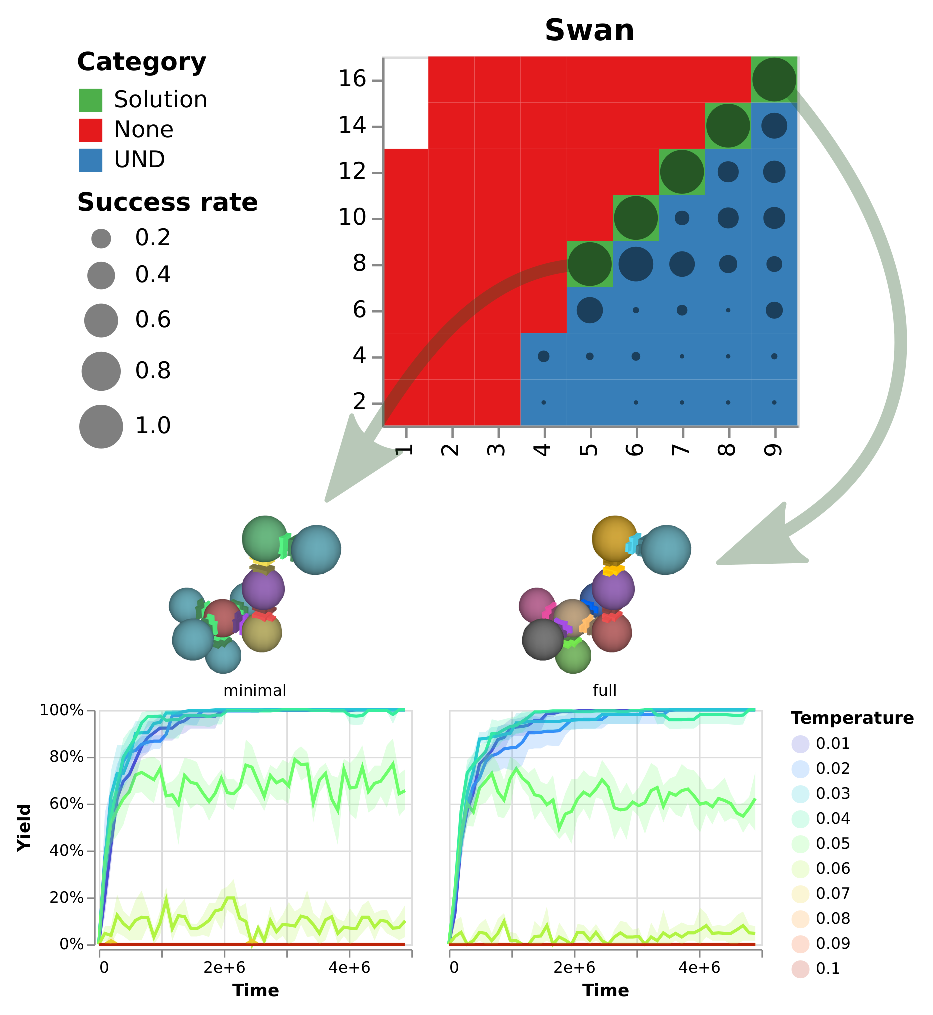
\includegraphics[width=\linewidth]{figures/patchysim/swanKinetics.eps}
    \caption{Assembly kinetics for different designs of the ``Swan'' shape. The left column shows the  \href{https://akodiat.github.io/polycubes/?assemblyMode=stochastic&rule=89010204000099099e00a20c0101861000000115920000009501020000000119020000000101021c0000010102000020010102008e00}{fully addressable solution} while the right is the \href{https://akodiat.github.io/polycubes/?assemblyMode=stochastic&rule=8f0b080b000b0b00000012008791000000000c0005000000000088000000}{minimal solution} found. Solid lines are mean values from 5 duplicate simulations, error bands show the 95\% confidence interval band. Each simulation is done using the narrow type \(0\) potential (patch width = \(2.346\)) at a \(0.1\) particle density. Temperature and time is measured in simulation units.}
    \label{fig:swanKinetics}
\end{figure}

\begin{figure*}[ht]
    \centering
    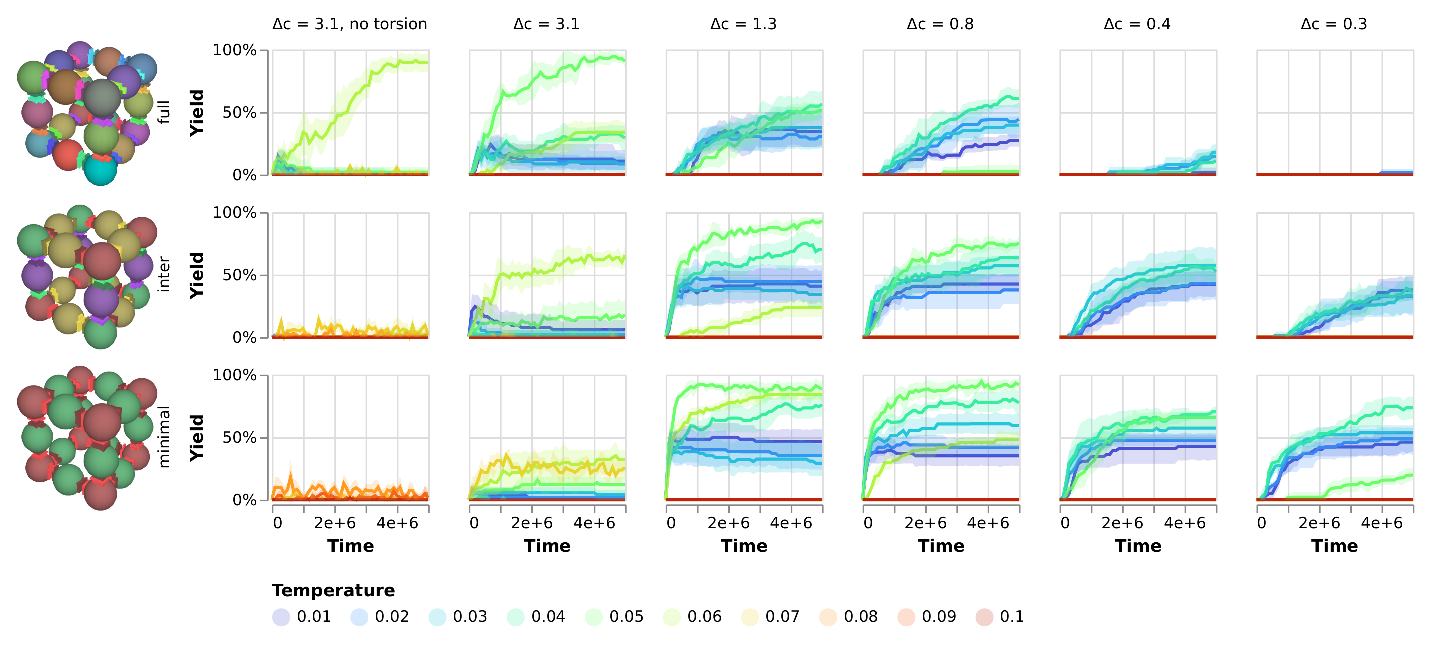
\includegraphics[width=\linewidth]{figures/patchysim/cubePotentials.eps}
    \caption{Assembly yield for hollow \(3 \times 3 \times 3\) cube designs. The top row shows the \href{https://akodiat.github.io/polycubes/?assemblyMode=stochastic&rule=00040109020c000089110200001491010218000001018e1c002001259e000000a5290200002ca901b200000001019a30963401010200863801010200ba00013d02400000bd450200b600c5010248ae4c01010200ce00e101d20000000101ca5000000101c254de000159d600a25c010102000000d9610200}{fully addressable solution}, using 20 species and 24 colours. The middle row shows an \href{https://akodiat.github.io/polycubes/?assemblyMode=stochastic&rule=90000800000600040090000d000000008b8d000011860000}{intermediate solution}, using 4 species and 4 colours. The bottom row shows the \href{https://akodiat.github.io/polycubes/?assemblyMode=stochastic&rule=070000070500868700000000}{minimal solution}, using 2 species and 1 colour. Columns correspond to different interaction potentials, with the leftmost column showing wide patches without torsion. The remaining columns show torsional patches with decreasing patch width. Solid lines are mean values from 5 duplicate simulations, and error bands show the 95\% confidence interval band. Each simulation has a \(0.1\) particle density.}
    \label{fig:cubePotentials}
\end{figure*}

\begin{figure*}[ht]
    \centering
    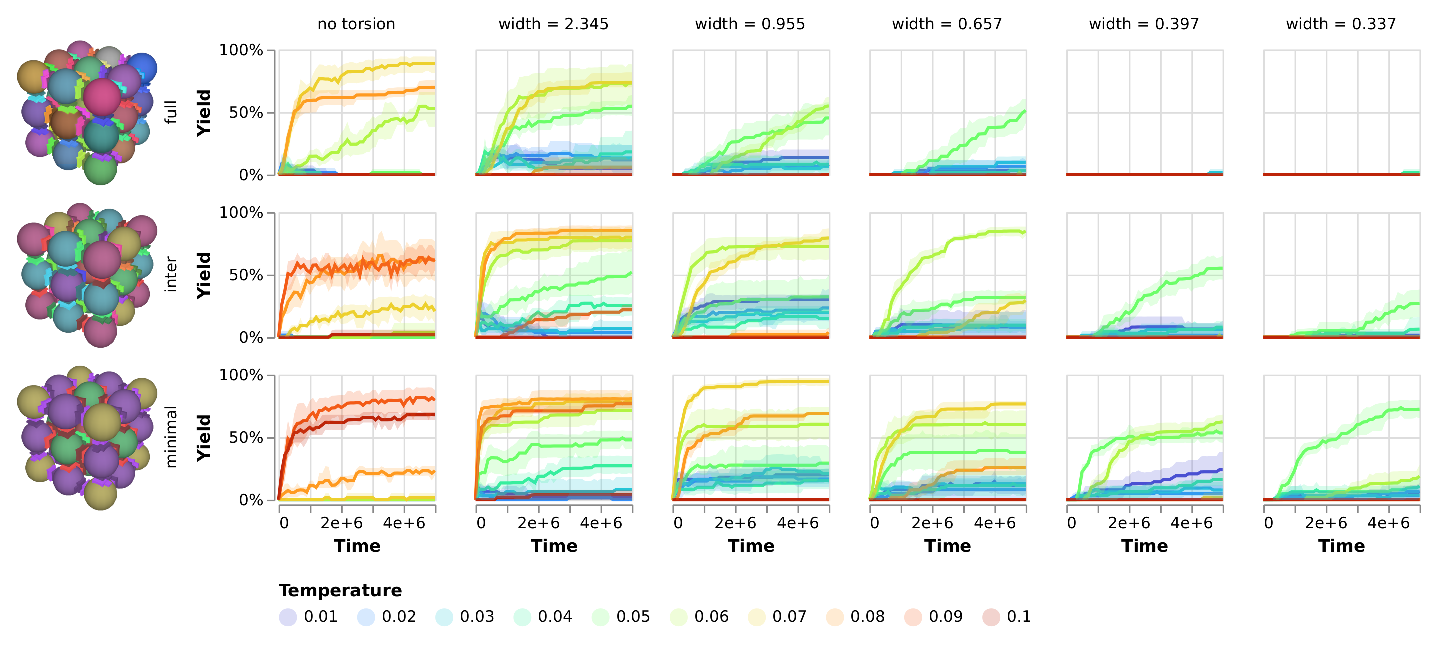
\includegraphics[width=\linewidth]{figures/patchysim/solidCubePotentials.eps}
    \caption{Assembly yield for solid \(3 \times 3 \times 3\) cube designs. The top row shows the \href{https://akodiat.github.io/polycubes/?decRule=|1:0||2:1||3:0_-1:2|4:0||5:1||6:0_|7:0|-2:1|8:1||9:0_|10:0||11:1|-3:2|12:0_-4:2|||13:1||14:0_-7:2|15:0|-5:1|16:1||17:0_-10:2|18:0||19:1|-6:2|20:0_-15:2||-13:1|21:1||22:0_-18:2|||23:1|-14:2|24:0_|25:0|-11:1|26:1|-9:2|27:0_|28:0||29:1|-12:2|_-25:2|30:0|-19:1|31:1|-17:2|32:0_-28:2|33:0||34:1|-20:2|_-30:2||-23:1|35:1|-22:2|36:0_-33:2|||37:1|-24:2|_|38:0|-29:1|39:1|-27:2|_-38:2|40:0|-34:1|41:1|-32:2|_-40:2||-37:1|42:1|-36:2|_|43:0|-8:1|||44:0_-43:2|45:0|-16:1|||46:0_-45:2||-21:1|||47:0_|48:0|-26:1||-44:2|49:0_-48:2|50:0|-31:1||-46:2|51:0_-50:2||-35:1||-47:2|52:0_|53:0|-39:1||-49:2|_-53:2|54:0|-41:1||-51:2|_-54:2||-42:1||-52:2|}{fully addressable solution}, using 27 species and 54 colours. The middle row shows an \href{https://akodiat.github.io/polycubes/?assemblyMode=stochastic&rule=10101113232391001d1d8c2400a2949495970c00a5001b1a1700009d0a8598008a000400}{intermediate solution}, using 6 species and 9 colours. The bottom row shows the \href{https://akodiat.github.io/polycubes/?assemblyMode=stochastic&rule=0a0a0b0a0908878784868b00060000078e8f000c0c00000e}{minimal solution}, using 4 species and 3 colours. Columns correspond to different interaction potentials, with the leftmost column showing wide patches without torsion. The remaining columns show torsional patches with decreasing patch width. Solid lines are mean values from 5 duplicate simulations, and error bands show the 95\% confidence interval band. Each simulation has a \(0.1\) particle density.}
    \label{fig:solidCubePotentials}
\end{figure*}

\begin{figure}[ht]
    \centering
    \begin{overpic}[width=\textwidth]{figures/patchysim/narrow_types.eps}
        \put(-10,210){a)}
        \put(210,210){b)}
    \end{overpic}
    \caption{Simulation of a pre-assembled patchy particle cube. \textbf{a)} The minimal solution to the hollow \(3 \times 3 \times 3\) from Figure~\ref{fig:hollow_cube}. \textbf{b)} Potential energy over time for different narrow types and temperatures.}
    \label{fig:narrow_types}
\end{figure}


Next, we then try to simulate and compare the assemblies of the fully addressable and minimal solutions to the shapes introduced in Section~\ref{sec:example_solves}. All the following simulations are run with narrow type 0.

%Looking at Figure~\ref{fig:patchy_energy}, there are temperatures for which each of the shapes start to nucleate early on, as a sudden drop in the energy over time corresponds to a nucleation event.

%\begin{figure}[ht]
%    \centering\includesvg[width=\textwidth, inkscapelatex=false]{figures/patchysim/energy.svg}
%    \caption{Potential energy over time in patchy particle simulations. The top row shows the fully addressable solution while the bottom row is the minimal solution found. Each simulation is done using the narrow type \(0\) potential at a \(0.1\) particle density.}
%    \label{fig:patchy_energy}
%\end{figure}

We can now look at the assembly yield, shown in Figure~\ref{fig:complete_clusters} as the percentage of clusters having the correct number of each species. Despite the aggregation previously discussed, the two cube shapes have a growing number of correct assemblies for certain temperatures. Meanwhile, the other shapes are all approach a high assembly yield for lower temperatures.

\begin{figure}[ht]
    \centering\includesvg[width=\textwidth, inkscapelatex=false]{figures/patchysim/complete_clusters.svg}
    \caption{Assembly yield over time for patchy particle simulations. The top row shows the fully addressable solution while the bottom row is the minimal solution found.Each simulation is done using the narrow type \(0\) potential at a \(0.1\) particle density.}
    \label{fig:complete_clusters}
\end{figure}

Another measure is the size of the clusters in the system, where a cluster is a set of particles joined through their patches. In Figure~\ref{fig:max_cluster}, we measure the normalised size of the largest cluster found, where 100 per cent is the intended size of the polycube. 

While the other shapes do not assemble any larger than the intended size, the two cubes aggregate into clusters many times larger than intended. \emph{This happens because these shapes are self-limiting through their geometry, which works less well on flexible patchy particles compared to the rigid lattice of the stochastic assembler}. In contrast, the other shapes are self-limiting through their topology, with no loops in their connectivity graphs.

\begin{figure}[ht]
    \centering\includesvg[width=\textwidth, inkscapelatex=false]{figures/patchysim/largest_cluster_size.svg}
    \caption{Largest cluster size over time for patchy particle simulations. The top row shows the fully addressable solution while the bottom row is the minimal solution found. Each simulation is done using the narrow type \(0\) potential at a \(0.1\) particle density.}
    \label{fig:max_cluster}
\end{figure}



A general remark on the simulation results in Figure~\ref{fig:patchy_energy}, \ref{fig:max_cluster}, and~\ref{fig:complete_clusters} is that there is usually not any significant difference between the assembly yields for the fully addressable solution (top row) and the minimal solution (bottom row). This means that experimental applications could use significantly fewer unique building blocks without the loss of money and time.

\section{Multifarious assemblies}

Another feature with the SAT solver approach is the ability to design \emph{multifarious} assemblies, that is, rules that can assemble into more than one shape. This is simply done by defining multiple distinct shapes next to each other as input to the solver.

Figure~\ref{fig:multifarious_rectangles} shows a solution landscape for two different rectangle shapes. The fully addressable solution (in the upper-right corner) has no shared species between the two shapes, while a simpler solution, such as: \href{https://akodiat.github.io/polycubes/?assemblyMode=stochastic&rule=0d01860000000501860000000905020000008d0102880000}{0d0186000000\allowbreak050186000000\allowbreak090502000000\allowbreak8d0102880000}
with \(\widetilde{K}_s=4\), \(\widetilde{K}_c=3\), share three out of four species.

\begin{figure}[ht]
    \centering\includesvg[width=\textwidth, inkscapelatex=false]{figures/solve/2rect.svg}
    \caption{Multifarious assembly of rectangles. Solution landscape (right) for the assembly of two different rectangular shapes (left).}
    \label{fig:multifarious_rectangles}
\end{figure}
%\begin{savequote}[8cm]
%A process cannot be understood by stopping it. Understanding must move with the flow of the process, must join it and flow %with it. (First Law of Mentat)
%  \qauthor{--- Frank Herbert, Dune}
%\end{savequote}
%Edsger W. Dijkstra, How do we tell truths that might hurt? (1975).

\chapter{\label{ch:oxview_intro}An introduction to tools for the design and simulation of nucleic acid structures}

\minitoc

While previous chapters have covered modular self-assembly on a very abstract level, approximating the modules as simple cubes or patchy particles, this chapter will introduce tools and methods for designing and simulating individual structures or modules folded using DNA (or RNA).

The following sections will cover a selection of practical design and simulation tools that have been developed over the years, providing context for the presentation of my contributions to the \emph{oxView} tool in Chapter~\ref{ch:oxview}.

% REFER TO THIS OVERVIEW!! https://pubmed.ncbi.nlm.nih.gov/33920889/


%Simulating the structure and dynamics of individual DNA origami modules has been possible for a while, but my aim with this project has been to make such simulations more accessible and easy to use and analyse.

%This is accomplished as I develop new tools and scripts while learning about the simulation methods and the designs that various laboratories are interested in.

%This chapter describes the currently available tools for simulation and design of individual module structures. DNA and RNA structures can be digitally represented in many different formats, for many different uses, and with different levels of coarse-graining. 

%The following sections cover my results over the last year, investigating methods for converting designs into the oxDNA/RNA format and for visualising and analysing the simulation results.

\section{Design tools}\label{sec:design_tools}
Designing a DNA origami structure by hand would be very laborious for anything but the most simple design. As such, a host of computer-aided design tools have been introduced over the years to make things easier. This section will cover some of the more common examples.

\subsection{Lattice-based design tools}
The caDNAno design tool \cite{cadnano} and the web-based scadnano \cite{scadnano} it inspired, allows the user to design DNA origami on a lattice of parallel helices.
\subsubsection{caDNAno}
\label{sec:cadnano}
CaDNAno \cite{cadnano} was introduced in 2009 as a way to simplify 2D and 3D DNA origami designs. It has a graphical user interface with multiple panels, seen in Figure~\ref{fig:cadnano}. In the slice panel, the designer can place virtual helices on a lattice (either hexagonal or square), seen in the leftmost panel of the figure. The helices can then be filled in with strands and connected using crossovers in a path panel, seen in the middle of the figure.

Finally, caDNAno is also available as a plugin to the Autodesk Maya software, which enables a 3D visualisation of the design as seen in the render panel to the right in Figure~\ref{fig:cadnano}. However, caDNAno does not support Maya versions after 2015 \cite{cadnanoInstall}.

\begin{figure}[h]
  \begin{center}
    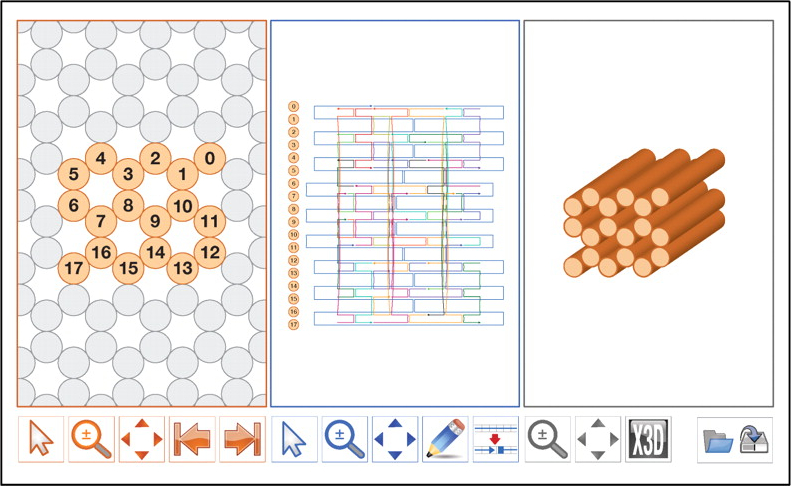
\includegraphics[width=0.6\textwidth]{figures/cadnano.jpeg}
    \caption{The caDNAno design interface, adapted from \cite{cadnano}. The slice panel (left) shows helices as circles on a lattice, while the path panel (centre) shows individual strands from a flatened side view of the helices. The rightmost panel shows a 3D visualisation of the design.}
    \label{fig:cadnano}
  \end{center}
\end{figure}

\subsubsection{Scadnano}
Scadnano \cite{scadnano} (scriptable caDNAno) is a relatively new design tool, independent from but inspired by caDNAno version 2. The main difference is that Scadnano is entirely web-based (thus not requiring any installation). The python code base is also designed to make it easier to write scripts generating DNA designs. Scadnano can be found at \url{https://scadnano.org/}.

\subsection{Top-down shape converters}
While tools like caDNAno simplify bottoms-up design, where the user builds structures from individual strands and nucleotides, a top-down tool can take a polyhedral target shape as input and provide a suitable origami design as output. 

% Mention DNA bricks software?

\subsubsection{BSCOR}
\label{sec:bscor}
%https://doi.org/10.1038/nature14586

In 2015, Benson et al. published a method for converting arbitrary mesh designs into a DNA origami mesh \cite{vHelix}. Figure~\ref{fig:bscor} shows a set of example polyhedral shapes, with the designed shape in \textbf{a)}, the output DNA design in \textbf{b)}, and microscopy characterisations in \textbf{c)}-d). A follow-up paper in 2016 also introduced the ability to design flat-sheet meshes \cite{benson2016computer}. BSCOR uses single DNA duplex edges, with double edges added whenever topologically necessary.

\begin{figure}[h]
  \centering
  \begin{overpic}[width=\textwidth]{figures/bscor.png}
    \put(20,460){\small{1. Mesh generation}}
    \put(280,460){\small{2. Scaffold routing}}
    \put(520,460){\small{3. Spring relaxation}}
    \put(780,460){\small{4. Staple design}}
    \put(-30,550){a)}
    \put(-30,350){b)}
    \put(-30,210){c)}
    \put(-30,70){d)}
  \end{overpic}
  \caption{3D meshes rendered in DNA origami using BSCOR. Adapted from \cite{vHelix} and \cite{vHelixWeb}. \textbf{a)} Automated design process, where a scaffold is routed onto a mesh, each helix is relaxed using spring forces, and staple strands are added. \textbf{b)} Examples of initial meshes. \textbf{b)} Completed DNA designs with strands rendered as tubes. \textbf{c)} Negative-stain dry-state TEM micrographs of each design.}
  \label{fig:bscor}
\end{figure}


\subsubsection{ATHENA}
% DAEDAULS/PERDIX
%https://www.science.org/doi/full/10.1126/science.aaf4388
 %ATHENA? https://academic.oup.com/nar/advance-article/doi/10.1093/nar/gkab762/6368527 - Use fig 2 in now published paper!!!

 ATHENA is a recently published tool for automatic design wireframe origami shapes. As seen in Figure~\ref{fig:athena}, earlier software such as PERDIX, METIS, DAEDALUS and TALOS has facilitated design for 2D and 3D wireframes using different edge designs but ATHENA aims to bring them all together as a single package.


\begin{figure}[h]
  \begin{center}
    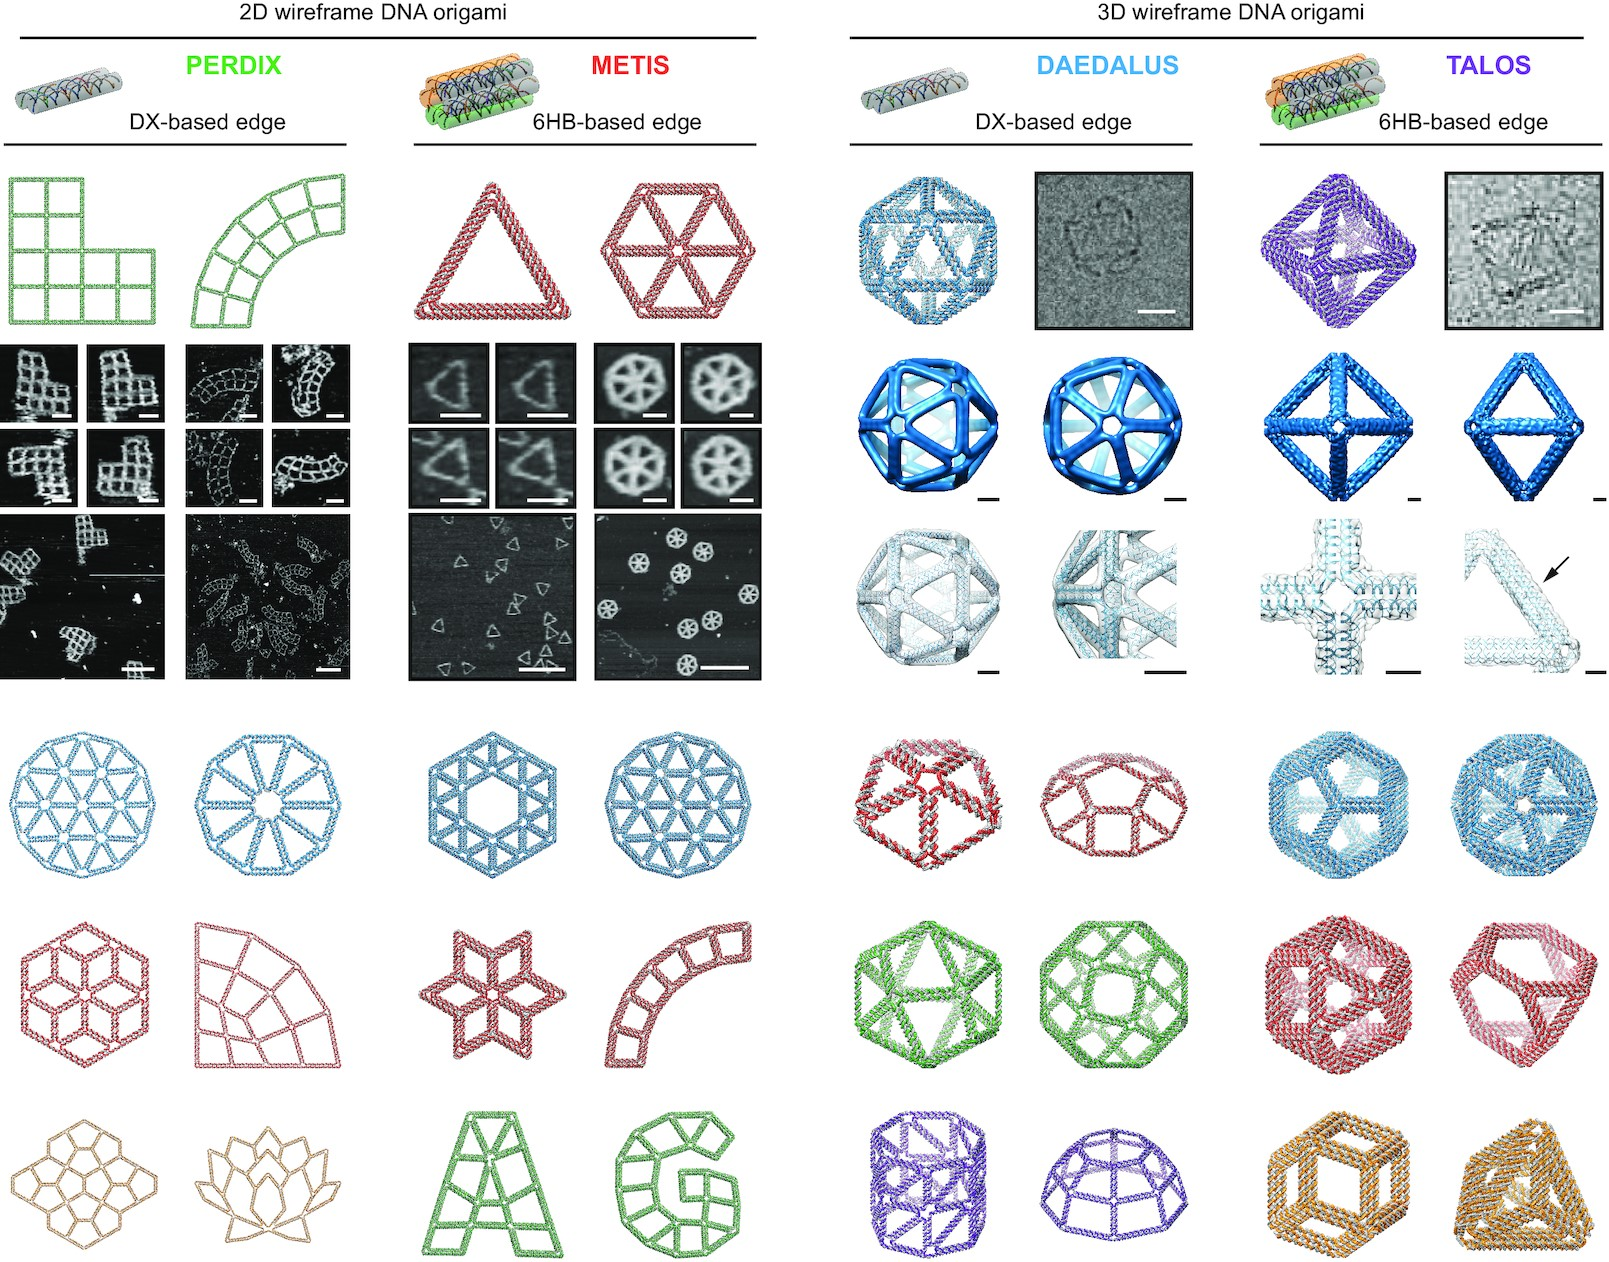
\includegraphics[width=\textwidth]{figures/athena.jpeg}
    \caption{Automatic wireframe origami shapes using ATHENA. Adapted from \cite{athena}. ATHENA includes the previous design packages PERDIX, METIS DAEDALUS and TALOS for 2D and 3D wireframe design, using double crossover (DX) and six-helix bundle (6HB) edges respectively. }
    \label{fig:athena}
  \end{center}
\end{figure}

%\subsubsection{Triangulated truss structures}
% M. Matthies
% https://pubs.acs.org/doi/abs/10.1021/acs.nanolett.6b00381

\subsection{Free-form or hybrid tools}
The final category of design tools is either free-form, where designs are drawn without a lattice, or hybrid tools combining both lattice and free-form design. 

\subsubsection{Tiamat}
Tiamat is an early free-form design tool introduced in 2009 \cite{Tiamat}, running on Microsoft Windows. See Figure~\ref{fig:tiamat} for a screenshot of the user interface of Tiamat 2, where a DNA tetrahedron is being designed. Tiamat can also import DNA from PDB files.

\begin{figure}[h]
  \begin{center}
    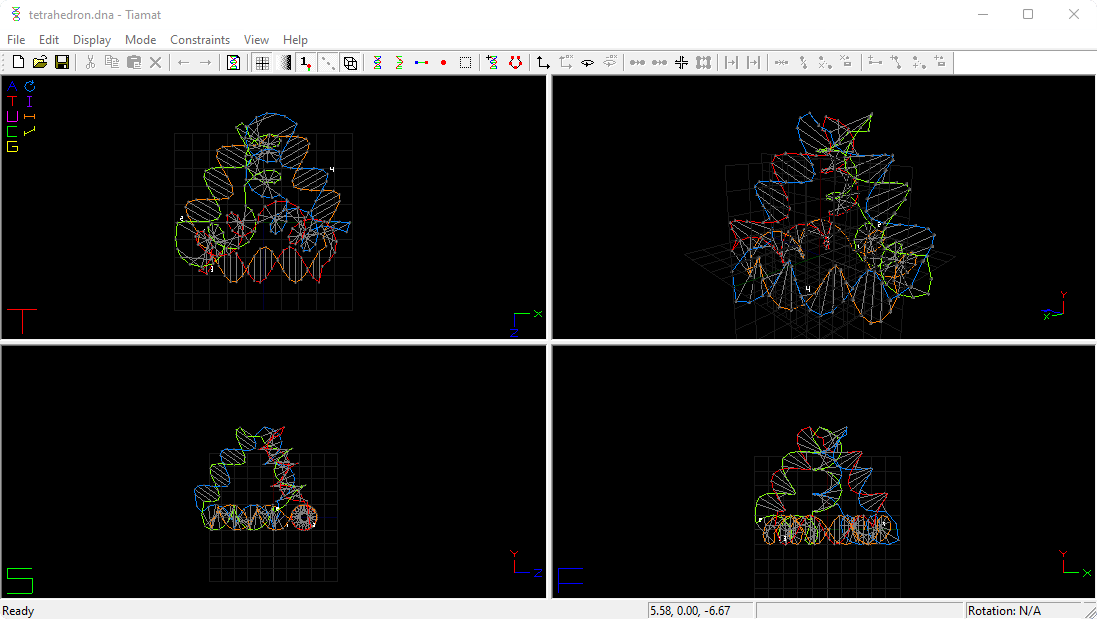
\includegraphics[width=\textwidth]{figures/tiamat_ui.png}
    \caption{A screenshot of the Tiamat \cite{Tiamat} (v2) user interface. The loaded tetrahedron design is from the Yan Lab resources page \cite{tiamatWeb}}
    \label{fig:tiamat}
  \end{center}
\end{figure}

\subsubsection{vHelix}
\label{sec:vhelix}
The free-form tool vHelix \cite{vHelix} is a plugin for the Autodesk Maya software and was developed together with the BSCOR toolkit. Users can import the ``rpoly'' wireframe result from BSCOR, create designs from scratch, or import caDNAno files. It is also possible to export oxDNA simulation files. An example of the vHelix interface is shown in Figure~\ref{fig:vhelix}. 

\begin{figure}[h]
  \begin{center}
    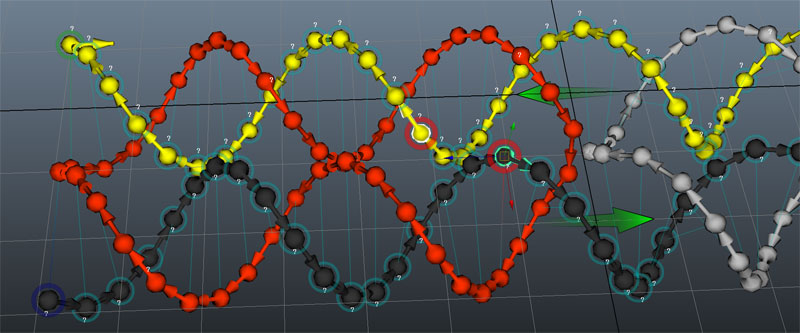
\includegraphics[width=\textwidth]{figures/vhelix.jpg}
    \caption{Free-form editing in vHelix. Image is from the vHelix website \url{http://www.vhelix.net/} \cite{vHelixWeb}.}
    \label{fig:vhelix}
  \end{center}
\end{figure}


\subsubsection{Adenita}
Adenita \cite{miao_tvcg_2018} is a free-form editing tool developed as a plugin to the SAMSON toolkit. As seen in Figure~\ref{fig:adenita}.a), the design can be visualised and edited at multiple levels of abstraction, from an all-atom representation, through nucleotides and strands to cylinders representing entire helices. Figure~\ref{fig:adenita}.b) shows some of the available editing and visualisation tools. Note, for example, the wireframe creation tool based on the Daedalus algorithm. Adenita can also load caDNAno files and export oxDNA simulation files.

Like vHelix (Section~\ref{sec:vhelix}), Adenita is tied to the commersial editor it is a plugin to.


\begin{figure}[h]
  \begin{center}
    \begin{overpic}[width=\textwidth]{figures/adenita.jpg}
      \put(-20,400){a)}
      \put(-20,100){b)}
    \end{overpic}
    \caption{Adenita, adapted from \cite{miao_tvcg_2018}. \textbf{a)} A DNA double-helix visualised at different abstraction levels, with a purple band highlihghting a specific base-pair at all the four main levels. \textbf{b)} Available editing and visualisation tools in Adenita.}
    \label{fig:adenita}
  \end{center}
\end{figure}

\subsubsection{MagicDNA}
MagicDNA \cite{huang2021integrated}, as seen in Figure~\ref{fig:magicDNA}, has a computer-aided design workflow where geometry can be specified from helix cross-sections or imported from a part library, then assembled into an integrated structure (using multiple scaffolds if necessary). MagicDNA is built as an application for the MATLAB software, so (like the previous two tools) installation requires a commersial third-party tool.


\begin{figure}[h]
  \begin{center}
    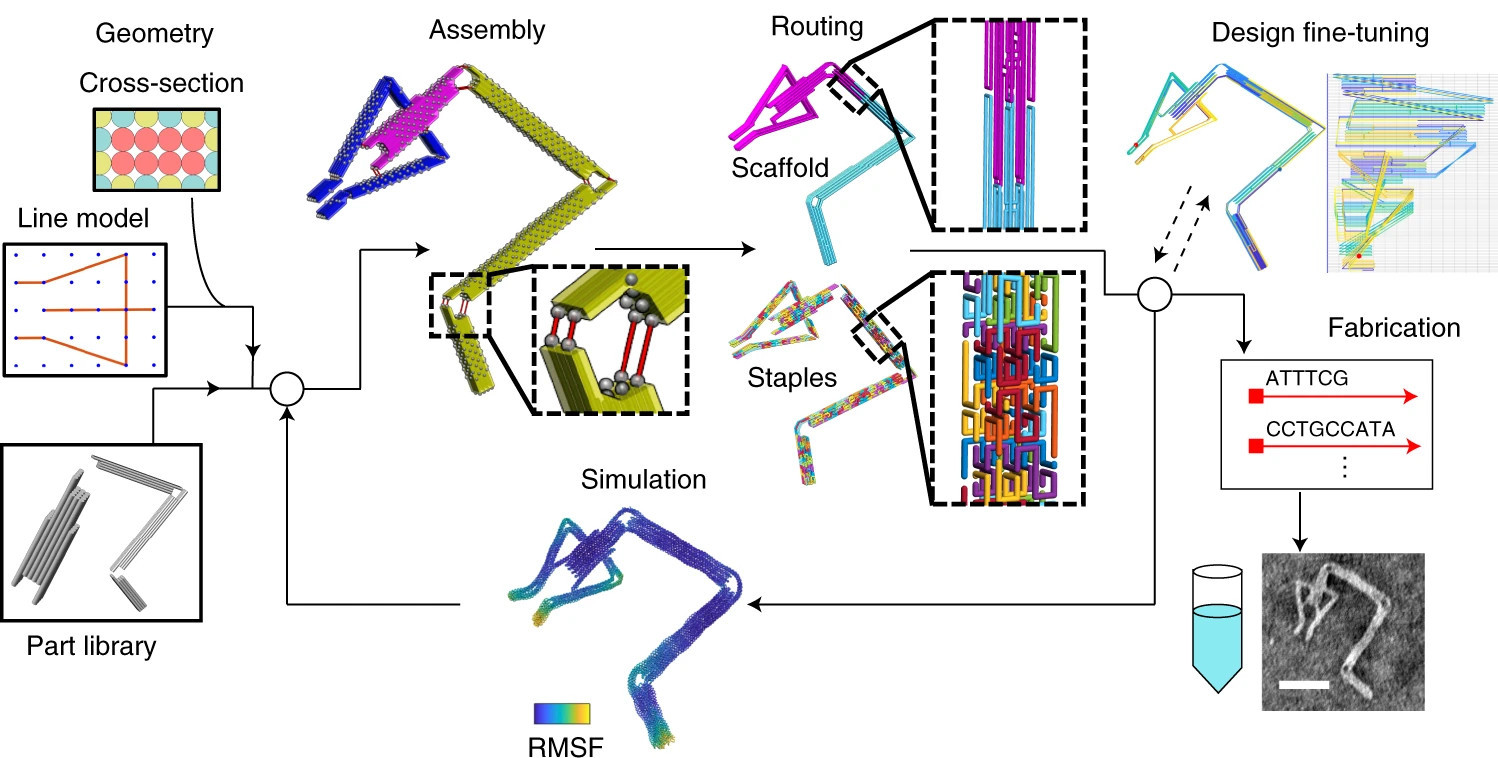
\includegraphics[width=\textwidth]{figures/magicDNA.jpeg}
    \caption{MagicDNA design workflow, adapted from \cite{huang2021integrated}. Assemblies can be created from line drawings and helix cross sections or imported from a library of parts. After strand routing and some optional fine-tuning in caDNAno, designs can be exported as sequences for fabrication or oxDNA files for simulation.}
    \label{fig:magicDNA}
  \end{center}
\end{figure}

\subsubsection{OxView}
The oxView application was developed as part of this thesis project and will be described more in Chapter~\ref{ch:oxview}.

\section{Simulation models}
Simulating a structure can provide insight to understand experimental results but can also guide decisions at the design stage. More coarse-grained models tend to run faster, but may lose some accuracy compared to models with more detail. This section covers simulation models at an increasing level of coarse-graining, from individual atoms to cylindrical helices.

\subsection{All-atom simulation}
Simulation tools such as NAMD \cite{NAMDphillips2005scalable}, use force fields such as AMBER \cite{AMBERcornell1996second} and CHARMM \cite{brooks1983charmm} that model interactions between individual atoms. While it is possible to perform atomistic simulations of large DNA origami structures \cite{yoo2013situ} as shown in Figure~\ref{fig:all-atom}, the simulations take a long time to run, and it is unknown how well the models represent DNA thermodynamics \cite{sengar2021primer}.

%Also cite Pointer origami https://academic.oup.com/nar/article/44/7/3013/2467847 ?

\begin{figure}[h]
  \begin{center}
    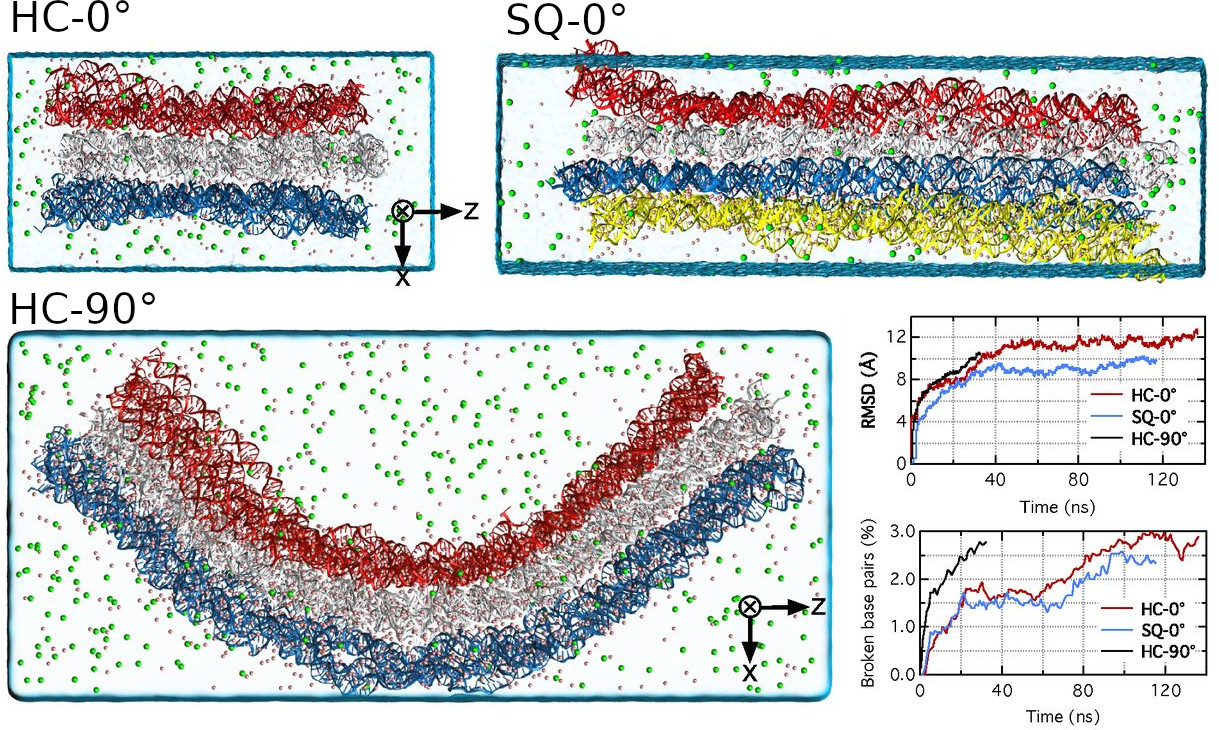
\includegraphics[width=\textwidth]{figures/all-atom.jpg}
    \caption{All-atom simulation of three DNA origami structures, adapted from \cite{yoo2013situ}. HC-0$^{\circ}$ is a honeycomb (hexagonal) lattice origami with no programmed curvature, while SQ-0$^{\circ}$ is designed on a square lattice. HC-0$^{\circ}$ has a programmed 90$^{\circ}$ bend. The plots show the root-mean-square deviation from the original atom positions (top) and the fraction of base pairs broken during the simulation (bottom).}
    \label{fig:all-atom}
  \end{center}
\end{figure}

\subsection{oxDNA/RNA}
\label{sec:oxDNA}
In 2010, a coarse-grained simulation software called oxDNA was introduced by Thomas Ouldridge \cite{ouldridge2010dna}. It simulates DNA on the level of nucleotides and has been shown to model complex origami devices with a generally good agreement with experimental data \cite{sharma2017characterizing}. In 2014, the DNA model was extended to include RNA by Petr {\v{S}}ulc \cite{vsulc2014nucleotide}, showing its ability to model a set of common RNA motifs. 

Molecular Dynamics (MD) and Monte Carlo (MC) simulation techiniques.

OxDNA was joined by cogli1 for trajectory visualisation.


% Mention ANM model by Jonah!!!

While oxDNA can be very useful for modelling a structure, it has traditionally not been very accessible for experimentalists. % mention web server

\begin{figure}[h]
\begin{center}
    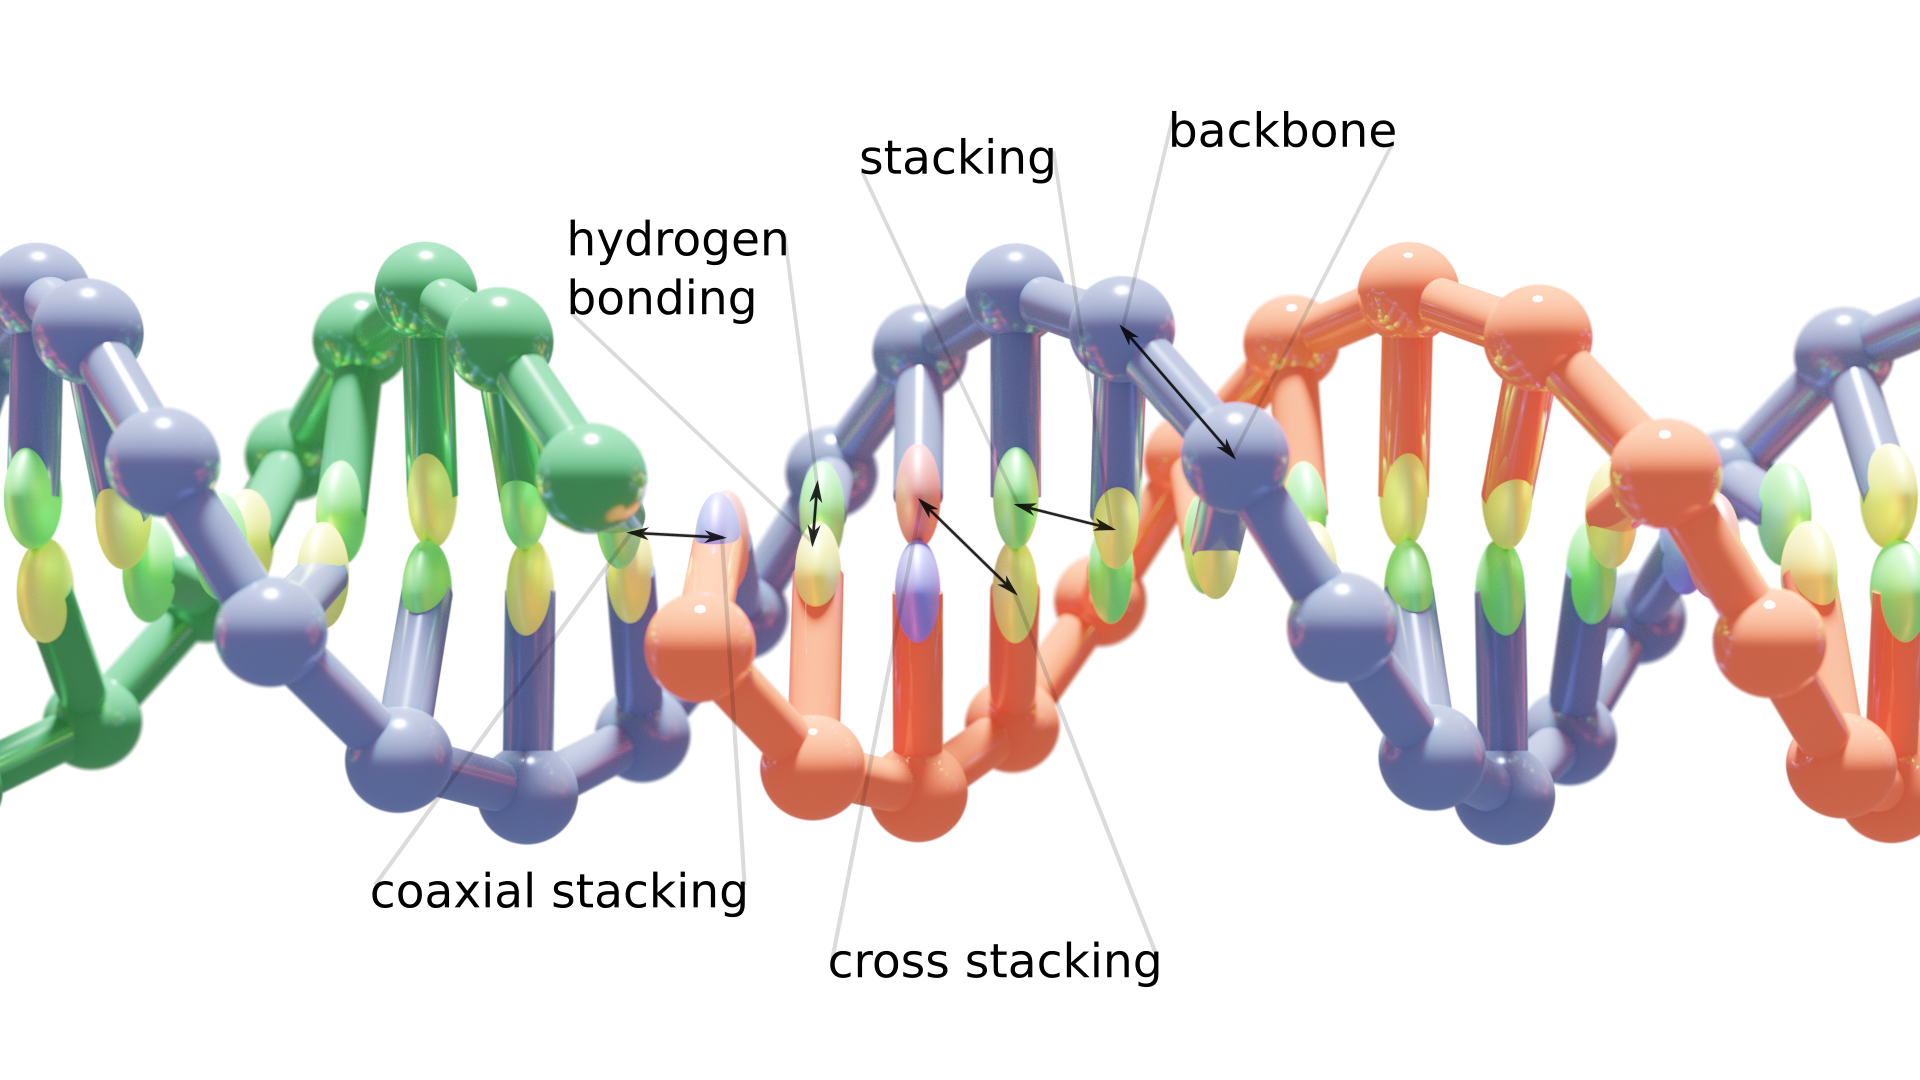
\includegraphics[width=\textwidth]{figures/oxdna_annot.png}
    \caption{The oxDNA model}
    \label{fig_oxDNA}
    \end{center}
\end{figure}

\subsection{mrDNA}
The mrDNA simulation model is a multi-resultion model representing a user-defined number of base-pairs as a rigid-body bead.

Since mrDNA is implemented in Python and has a spline-based helix representation, users can write scripts to edit the structure, translating and rotating parts before starting the simulation. Thus, topological issues or over-stretched bonds can, with some skill, be resolved even before starting to simulate.

I did, based on this, also create a rudimentary interactive editor interface to mrdna, but it would need a lot of refinement to be externally usable. More importantly, the oxView editor described in Chapter~\ref{ch:oxview} can now easily resolve these issues.

\begin{figure}[h]
  \begin{center}
    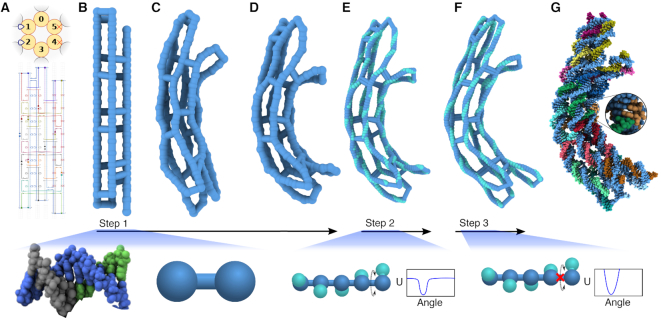
\includegraphics[width=\textwidth]{figures/mrDNA.jpg}
    \caption{MrDNA}
    \label{fig:mrdna}
  \end{center}
\end{figure}

A selection of the DNA designs I have relaxed are shown in Figure~\ref{fig:oxDNA_sims}. The first two examples, adopted from \cite{gerling2015dynamic} and \cite{zadegan2012smallbox} and illustrated in Figure~\ref{fig:oxDNA_sims}.a and~\ref{fig:oxDNA_sims}.b, are both quite straightforward to relax in oxDNA, although the relaxation is much faster using mrdna.

The tensegrity kite structure, adopted from \cite{liedl2010_kite} is harder to relax since, as seen in the first image in Figure~\ref{fig:oxDNA_sims}.c, the two helix bundles are drawn parallel to each other in caDNAno. Given enough time to relax, they should still become orthogonal, but a much more efficient way is to write a mrdna script to rotate one helix bundle so that it is orthogonal from the start, as seen in the middle image of~\ref{fig:oxDNA_sims}.c. The remaining overstretched bonds are then quickly relaxed using mrdna.

Finally, the Möbius strip, adopted from \cite{han2010moebius}, is particularly tricky to relax, since the caDNAno design have all helices drawn in the same plane, with bonds from each end stretching through the whole structure and intersecting at a single point, as can be seen in the first image of Figure~\ref{fig:oxDNA_sims}.d. With some help from Chris Maffeo, however, I was able to use a mrdna script to edit the structure into a configuration much easier to relax, as seen in the second image of Figure~\ref{fig:oxDNA_sims}.d. Since the caDNAno design does not make it clear if the Möbius strip should be left-handed or right-handed, this is also decided in the script; changing the rotational direction will produce a mirrored version of the structure, as seen in the third image of Figure~\ref{fig:oxDNA_sims}.d.

\begin{figure}
  \centering
  \begin{overpic}[width=\textwidth]{figures/oxdna_sims.eps}
    \put(0,960){a)}
    \put(0,760){b)}
    \put(0,540){c)}
    \put(0,260){d)}
  \end{overpic}
  \caption{Relaxation results for various DNA designs. Each row depicts a new design, with the left-hand side showing the structure as it was drawn in caDNAno (and parsed by mrdna), while the right-hand side is the relaxed structure in oxDNA. Intermediate images are edits done in mrdna. While the switch design \cite{gerling2015dynamic} in  \textbf{a)} 
  and the small DNA origami box \cite{zadegan2012smallbox} in  \textbf{b)} relaxed without any required editing, the tensegrity kite structure \cite{liedl2010_kite} in  \textbf{c)} and the Möbius strip \cite{han2010moebius} in  \textbf{d)} benefited greatly from moving selected helices to a position off the lattice before starting the simulation.}
  \label{fig:oxDNA_sims}
\end{figure}

\subsection{Cando}

Cando is a finite element modelling framework \cite{castro2011primer, kim2012cando} available through a web server at \url{https://cando-dna-origami.org}. DNA double helices are modelled as elastic rods (connected by rigid crossovers) that stretch, twist and bend in line with experimental measurements. See Figure~\ref{fig:cando} for a set of example structures designed in caDNAno and simulated in Cando.

\begin{figure}[h]
  \begin{center}
    \begin{overpic}[width=\textwidth]{figures/cando.png}
      \put(0,670){a)}
      \put(500,670){b)}
      \put(0,300){c)}
      \put(810,300){d)}
    \end{overpic}
    \caption{Cando simulation results. Adapted from \cite{castro2011primer}. CaDNAno design diagrams, Cando structure and flexibility prediction, and negative-stain TEM micrographs \textbf{a)} 90 degree gear. \textbf{b)} 180 degree gear. \textbf{c)} ``Robot'' design \textbf{d)} 60-helix bundle.}
    \label{fig:cando}
  \end{center}
\end{figure}
\chapter{\label{ch:oxview}Structure design and analysis in oxView}

\minitoc

This chapter contains my results on my second project: how to design, simulate and analyse DNA and RNA nanostructures. 

%It starts with an introductory description of earlier approaches to this problem and will then describe how my contributions to the oxView tool have improved the previous methods and enabled new results.

As I started this DPhil, I was tasked with the issue of converting origami designs created in caDNAno (see Section~\ref{sec:cadnano}) so that they could be correctly simulated in oxDNA (see Section~\ref{sec:oxDNA}). I collaborated with Hannah Fowler from the Doye group at Theoretical Chemistry, who simulated an extensive collection of old DNA designs. This was a good opportunity to investigate why some structures were more problematic to convert and relax than others.

At this time, the available method for converting a caDNAno design into the oxDNA format was to use an old python script included in the UTILS directory of the oxDNA repository. However, the script was not easy to use, and it failed for many structures. At the end of 2018, the tacoxDNA webserver \cite{suma2019tacoxdna} was launched, updating the conversion script and making it more accessible.

Still, since caDNAno structures are drawn on a lattice, where all helices have to be parallel to each other, the resulting oxDNA configurations often had unnaturally extended backbone bonds, requiring time-consuming relaxation.

During a secondment within the {\v{S}}ulc group at Arizona State University in 2019, I was able to contribute to their development of a web-based oxDNA viewer called oxView \cite{poppleton2020design, bohlin2021design}. This tool can now be accessed at {\large\url{www.oxview.org}}.

Among the main early features that I added to oxView was a cluster-level rigid-body dynamics option (detailed in Section~\ref{sec:rigid-body_dynamics}) that, in many cases, speed up the relaxation by orders of magnitude compared to oxDNA relaxation alone. Since then, I have collaborated with the {\v{S}}ulc group to add more features and to make the tool more accessible as a visualiser and editor. 

For our second oxView publication \cite{bohlin2021design}, I rewrote the main parts of the taxoxDNA codebase into TypeScript, resulting in the \emph{taxoxdna.js} library (\url{https://github.com/Akodiat/tacoxdna.js}) which oxView now uses to import various standard design formats (including caDNAno) automatically. This is described in Section~\ref{sec:importing_designs}.

This chapter will present my own contributions to oxView \cite{poppleton2020design, bohlin2021design}, unless otherwise stated. However, I wish to acknowledge the work done by Erik Poppleton and Michael Matthies; without them, this tool would not exist. Michael was the original oxView developer and has done great work in supporting live oxDNA relaxations through the \emph{ox-serve} webserver. Erik enabled oxView to render and analyse systems with over a million nucleotides and has created a large set of useful analysis scripts. Aamik Mallya and Jonah Procyk have also made significant contributions to the oxView codebase. 

\section{Importing designs}
\label{sec:importing_designs}
There are many different formats available for DNA origami design; some of the main design tools producing them are covered in Section~\ref{sec:design_tools}. This section will describe how to use oxView to import designs from such tools.

\subsection{Basic import}
Thanks to the \emph{tacoxdna.js} library, importing designs is now generally straightforward. An import button in the ``file'' menu allows the user to import caDNAno, rpoly and tiamat (json) files, while oxDNA and PDB files can be directly opened. Some additional formats still require the use of the external Tacoxdna webserver \cite{taco}. Any loaded structure can then be exported for oxDNA simulation, as described in Section~\ref{sec:oxdna_export}.

\subsubsection{Importing caDNAno files}
JSON files created using caDNAno (described in Section~\ref{sec:cadnano}) can now be imported directly into oxView. See the import dialog shown in Figure~\ref{fig:cadnano_import}.a). First, select the file to import and make sure to also select \emph{caDNAno} as the file format. Next, choose the correct lattice-type; either \emph{Square} or \emph{Hexagonal}. Optionally, input a sequence to assign to the origami scaffold (which will otherwise be random).

\begin{figure}[ht]
  \begin{center}
    \begin{overpic}[width=0.8\textwidth]{figures/oxview_import/import.eps}
      \put(-30,810){a)}
      \put(-30,530){b)}
      \put(-30,230){c)}
    \end{overpic}
    \caption{Importing caDNAno structues into oxView. \textbf{a)} The tacoxdna.js library import dialog in oxView (left), seen here importing a caDNAno design. Note the web browser console shown to the right, where any additional output from the import is written. \textbf{b)} Imported linear actuator rail design from \cite{benson2021strategies}. \textbf{c)} Complete linear actuator structure from \cite{benson2021strategies} assembled in oxView, after also importing the slider caDNAno design.}
    \label{fig:cadnano_import}
  \end{center}
\end{figure}

Another option is to use the tacoxdna webservice to convert the caDNAno design into oxDNA files and then load those into oxView. However, designs loaded directly into oxView have the benefit of including correct colouring, clustering and base-pairing information, which would otherwise have been lost.

\subsubsection{Importing rpoly files}
Rpoly files are the output from the BSCOR \cite{vHelix} tool (described in Section~\ref{sec:bscor}) for converting polyhedral meshes into DNA origami.
Select the rpoly file to import, making sure that \emph{rpoly} is selected as the file format. Optionally, input a sequence to assign to the origami scaffold (which will otherwise be random).

\subsubsection{Importing Tiamat files}
Tiamat (described in Section~\ref{sec:tiamat}) designs in the \emph{.dnajson} format can also be imported. Select file to import, making sure that \emph{tiamat} is selected as file format. Binary \emph{.dna} Tiamat files need to be reopened in Tiamat and saved to the text-based \emph{.dnajson}. Select Tiamat version (1 or 2), then select the nucleic acid type (DNA or RNA).

By default, nucleotides without assigned base types will be given a random type. However, it is also possible to select a fixed default base.

\subsubsection{Importing PDB files}
While I did include the DNA PDB to oxDNA converter from Tacoxdna in \emph{tacoxdna.js}, a more versatile PDB import was created by Jonah Procyk to support his ANM-oxDNA model \cite{procyk2021coarse}. Simply drag and drop (or load) a PDB file into an oxView window and the DNA, RNA and/or protein it contains will be automatically converted and loaded.

%The simplest method is now to use the recently published tacoxDNA web service \cite{suma2019tacoxdna} (whose conversion script is more or less the same as in the oxDNA repository). However, the script can still fail to parse some designs, so a future implementation that uses the native caDNAno library for parsing would be preferable.

\subsection{Multi-component designs}
Designs spread across multiple files (or even multiple design tools) can be easily combined in oxView by simply importing them all and using the editing tools to arrange and connect them properly. Figure~\ref{fig:cadnano_import} shows an example of this, where the a slider design (Figure~\ref{fig:cadnano_import}.c) is added and positioned relative to the already imported rail (Figure~\ref{fig:cadnano_import}.b), both structures from \cite{benson2021strategies}.

\subsection{Far-from-physical caDNAno designs}
Some structures, while converted without failure to the oxDNA format, will have a very far-from-physical configuration due to the way they are drawn in caDNAno. As mentioned in the begining of this chapter, since it is only possible to draw all helices parallel to each other (on a lattice), backbone bonds may be very elongated, creating high energies and/or topological problems.

The oxDNA software already includes relaxation procedures for such structures \cite{doye2020oxdna}, bringing them together in a slow and controlled manner using a specified maximum backbone force. However, for large structures, this can take a very long time, even while using GPU simulation.

As discussed in Section~\ref{sec:mrdna} and shown in Figure~\ref{fig:mrdna}, the mrDNA simulation model \cite{maffeo2019mrdna} can help in such cases. However, the easiest option now tend to be using oxViews editing and rigid-body dynamics capabilities.

\section{Rigid-body and dynamics}
\label{sec:rigid-body_dynamics}

For rapid relaxation of imported caDNAno designs, oxView includes so-called rigid-body dynamics. When the dynamics are active, clusters of nucleotides are treated as rigid-bodies in a simple physics simulation, using the method described in \cite{baraff1997introduction} and running locally in the web browser.

Clusters can be defined manually, or by running an automatic DBSCAN \cite{ester1996density} clustering algorithm. If caDNAno files are imported directly into oxView, they will already have clusters defined. Similarly, copying and pasting structures create separate clusters.

\begin{figure}[ht]
  \centering
  \begin{overpic}[width=\textwidth]{figures/icosahedron.png}
    \put(0,300){a)}
    \put(240,300){b)}
    \put(620,300){c)}
  \end{overpic} 
  \caption{Rigid-body dynamics of clusters. Snapshots from the automatic rigid-body relaxation of an icosahedron, starting with the configuration converted from caDNAno \textbf{a)}, through the intermediate  \textbf{b)} where the dynamics are applied, and \textbf{c)} the final resulting relaxed state.}
  \label{fig:rigidBody}
\end{figure}

Within the dynamics, clusters are held together with spring forces at each shared backbone bond, with a magnitude of \(f_{\rm spr} = c_{spr}(l - l_r)\)
where \(c_{spr}\) is a spring constant, \(l\) is the current bond length and \(l_r\) is the relaxed bond length. To avoid overlaps, a simple linear repulsive force, of magnitude
\(f_{\rm rep} = max\left(c_{rep}\left(1-\frac{d}{r_a+r_b}\right),0\right)\) is added between the centre of each group, where \(c_{rep}\) is a repulsion constant, \(d\) is the distance between the two centres of mass, and \(r_a+r_b\) is the sum of the group radii (the greatest distance they can be while still overlapping).

As seen in Figure~\ref{fig:rigidBody}, the separate clusters will relax into a more natural shape, prepared for oxDNA simulation or further design. In some cases, however, simply moving the clusters manually (rigid-body manipulation) might be an even easier solution, which brings us to the section on editing.

\section{Editing designs}

\begin{figure}[ht]
\begin{overpic}[width=\textwidth]{figures/tetra.eps}
  \put(0,200){a)}
  \put(200,200){b)}
  \put(470,200){c)}
  \put(740,200){d)}
\end{overpic}
\caption{Designing the DNA tetrahedron from \cite{goodman2005rapid} using the oxView editing tools. \textbf{a)} An initial 20 base pair helix created. \textbf{b)} Duplicated helices being rotated and translated into place. \textbf{c)} Strands ligated together. \textbf{d)} The resulting 3D tetrahedron shape, as seen after applying rigid-body dynamics.}
\label{fig:design}
\end{figure}

While oxView started as a visualisation tool, it has since been extended with a number of editing features. One of the earliest was the ability to perform rigid-body manipulation of selected nucleotides by dragging them with the mouse. I contributed by adding transformation gizmos that simplify translation and rotation of selections using on-screen arrows and arcs for the user to manipulate. See Table~\ref{table:edit_tools} for a complete list of the editing tools currently available in oxView.

With the ability to create, remove, connect, and disconnect nucleotides, oxView users can now design structures from scratch. See, for example, Figure~\ref{fig:design}, where the DNA tetrahedron from \cite{goodman2005rapid} is created. The user first creates an initial helix (Figure~\ref{fig:design}.a) by typing a 20-base sequence and clicking the ``Create'' button \includesvg[height=1em]{figures/tools/create} in the ``Edit'' menu. Note that the ``Duplex mode'' need to be active in order for the complementary strand to be created automatically. Next, the user can copy \includesvg[height=1em]{figures/tools/copy} and paste \includesvg[height=1em]{figures/tools/paste} the helix repeatedly, using the ``Translate'' \includesvg[height=1em]{figures/tools/translate} and ``Rotate'' \includesvg[height=1em]{figures/tools/rotate} tools to position the helices as seen in~\ref{fig:design}.b).

Any edit can also be undone and redone, either pressing Ctrl+Z or Ctrl+Z, or by pressing the corresponding buttons, \includesvg[height=1em]{figures/tools/undo} or \includesvg[height=1em]{figures/tools/redo}.

%ligate, nick, do/undo, extend and create strands

\newcommand{\toolHeight}{1.5em}


\begin{table}[ht]
\centering

\begin{tabularx}{\textwidth} { >{\centering\arraybackslash}m{3em} | X }
 \hline
 Tool & Description \\ [0.5ex] 
 \hline
 \hline
\includesvg[height=\toolHeight]{figures/tools/create} & \textbf{Create} a new strand from a given sequence. Select \textit{duplex mode} to instead create a helix. \\ \hline
\includesvg[height=\toolHeight]{figures/tools/copy} & \textbf{Copy} the selected elements (Ctrl+C). \\ \hline
\includesvg[height=\toolHeight]{figures/tools/cut} & \textbf{Cut} the selected elements (Ctrl+X). \\ \hline
\includesvg[height=\toolHeight]{figures/tools/paste} & \textbf{Paste} elements from clipboard (Ctrl+V to paste in original position, or Ctrl+Shift+V to paste in front of camera). \\ \hline
\includesvg[height=\toolHeight]{figures/tools/delete} & \textbf{Delete} all currently selected elements (delete). \\ \hline
\includesvg[height=\toolHeight]{figures/tools/ligate} & \textbf{Ligate} two strands by selecting the 3' and 5' endpoint elements to connect (L). \\ \hline
\includesvg[height=\toolHeight]{figures/tools/nick} & \textbf{Nick} a strand at the selected element (N) \\ \hline
\includesvg[height=\toolHeight]{figures/tools/extend} & \textbf{Extend} strand from the selected element with the given sequence. Select \textit{duplex mode }to also extend the complementary strand. \\ \hline
\includesvg[height=\toolHeight]{figures/tools/insert} & \textbf{Insert} (add) elements within a strand after the selected element. \\ \hline
\includesvg[height=\toolHeight]{figures/tools/skip} & \textbf{Skip} (remove)  selected elements within a strand. \\ \hline
\includesvg[height=\toolHeight]{figures/tools/rotate} & \textbf{Rotate} selected elements around their center of mass (R). \\ \hline
\includesvg[height=\toolHeight]{figures/tools/translate} & \textbf{Translate} currently selected elements (T). \\ \hline
\includesvg[height=\toolHeight]{figures/tools/moveto} & \textbf{Move to}. Move other selected elements to the position of the most recently selected element. \\ \hline
\includesvg[height=\toolHeight]{figures/tools/connect3s} & \textbf{Connect 3' duplex}. Connects the 3' ends of two selected staple strands with a duplex, generated from the sequence input. \\ \hline
\includesvg[height=\toolHeight]{figures/tools/connect5s} & \textbf{Connect 5' duplex}. Connects the 5' ends of two selected staple strands with a duplex, generated from the sequence input. \\ \hline
\includesvg[height=\toolHeight]{figures/tools/set} & \textbf{Set} the sequence of currently selected elements. Select duplex mode to also set the complementary sequence on paired elements. \\ \hline
\includesvg[height=\toolHeight]{figures/tools/get} & \textbf{Get}. Assigns the sequence of selected bases to the sequence input.  \\ \hline
\includesvg[height=\toolHeight]{figures/tools/rc} & \textbf{Reverse complement}. Generates the reverse complement of a provided sequence. \\ \hline
\includesvg[height=\toolHeight]{figures/tools/search} & \textbf{Search}. Highlights the position the provided sequence in each strand, if present. \\ \hline
\end{tabularx}

\caption{Editing tools available in oxView}
\label{table:edit_tools}
\end{table}



\section{Visualization options}
Depending on the design, a user of oxView might want to modify the visualisation settings to make certain features of the structure more or less visible.

\paragraph{Centring with periodic boundary conditions} A useful utility when visualising an oxDNA trajectory is to keep the structure centred at the origin, stopping it from drifting out of view. The method described in \cite{PBC_centring} was used to achieve centring while taking periodic boundary conditions into account.

% https://doi.org/10.1080/2151237X.2008.10129266
% https://en.wikipedia.org/wiki/

In essence, for each coordinate \(p_j = \left(p_x^j, p_y^j, p_z^j\right) \) in the centring set of size \(n\), each dimension \(i \in \left\{x,y,z\right\}\) gets averaged in its own variable \(\alpha_i\), representing its 1D interval as a 2D circle (where the circumference \(b_i\) is the bounding box side length):

\[
  c_i = \frac{1}{n} \sum_{j = 1}^{n} \left[ \cos \left( \alpha_i^j \right), \sin \left( \alpha_i^j \right) \right]  
\]

Here, \(\alpha_i^j = \frac{2 \pi}{b_i} p_i^j\) is the angle on the unit circle and \(c_i\) is the average 2D position representing dimension \(i\). Finally, the averages are converted back to cartesian coordinates:

\[
  cm_i = \pi + \frac{b_i}{2\pi} atan2(-c_{i,y}, -c_{i, x})
\]

\paragraph{Change component sizes} Depending on the structure scale, some visual components might be more or less common. This can be configured using the `Visible components' option in the ``View'' menu, where the nucleoside sphere, nucleoside connector, backbone sphere, and backbone connector components can be rescaled or hidden entirely.

\paragraph{Colours} Nucleotides can be coloured by system, cluster, strand or by custom colouring specified by the user or at import. Users can also configure the default color palette used in oxView. Finally, it is also possible show colour overlays from the analysis scripts, mostly developed by Erik Poppleton. 

\paragraph{Virtual reality} Understanding the 3D structure of a design shown on a 2D screen is not alwasy so easy. Some view options like enabling fog might help the depth perception a bit, but oxView is also compatible with webVR, enabling the user to inspect their design with a virtual reality (VR) headset. The button to enable VR can be found in the ``View'' menu.

\section{Exporting designs}
\label{sec:oxdna_export}
Once a structure has been created in or loaded into oxView, it can be exported in a variety of formats.

\subsection{Exporting oxDNA simulation files}
OxView can export topology, configuration, and external force files for oxDNA simulation. Simply click the ``Export oxDNA'' button in the ``File'' menu and select the required file types.

One important thing to note is that the oxDNA format requires nucleotides to be correctly sorted with consecutive indices. Furthermore, this sorting is done, against convention, in a 3' to 5' order. Meanwhile, to facilitate editing, oxView nucleotides keep their indices even if the topology changes. Thus, nucleotides indices may be reassigned on oxDNA export, so it is important to export all files (topology, configuration, and forces) if the design has been edited.

\subsection{Exporting other 3D formats}
File formats such as glTF and STL contain geometrical information that can be 3D printed or imported into other 3D software such as Blender. OxView exports the scene as it is at the moment of export (at the current frame if a simulation trajectory is loaded), so it is important to configure intended component sizes and colours beforehand.

\paragraph{STL} is an old and common standard for 3D shapes, containing only vertex coordinates (no colours). It is a popular input for 3D printing, but the file size is relatively large.

\paragraph{glTF} (or glb if binary) is a modern standard for 3D scenes, storing geometry, hierarchy, and even material properties.

\subsection{Exporting sequence files}
Strand sequences can be exported as standard CSV files using the ``Sequence file'' export button in the ``File'' menu. The designed sequences can then be ordered and assembled experimentally.

\subsection{Saving image files}\label{sec:image_export}

It is possible to save an image of the current oxView view by simply clicking the ``Save image'' button in the ``File'' menu. This is a preferred option over a screenshot for two reasons. First, it is possible to increase the resolution by a scaling factor found in the ``Image size'' dropdown (rescale the browser window to change the aspect ratio of the image). Secondly, the background of the saved image will be transparent, simplifying further editing and composition.

For cover art and photo-realistic renders, it is also possible to export and load a glTF file into (for example) Blender, as seen in Figure~\ref{fig:image_export}. Note that in current Blender versions (2.9), large structures take a long time to import. So, make sure to disable any components not needed before export.

\begin{figure}[ht]
  \centering
  \begin{overpic}[width=\textwidth]{figures/oxview_image_export/row.png}
    \put(0,280){a)}
    \put(320,280){b)}
    \put(670,280){c)}
  \end{overpic}
  \caption{Component scaling and image export. \textbf{a)} Default oxView visualisation. \textbf{b)} Custom component scale and visibility. Using the``Visible components'' dropdown in the ``View'' menu,  the backbone spheres have been scaled up by a factor of 4.18 while all other nucleotide components have been hidden. \textbf{c)} The scaled scene in \textbf{b)} exported as glTF and rendered using Cycles in Blender.}
  \label{fig:image_export}
\end{figure}

\subsection{Creating videos}
One of the earlier features I implemented in oxView was the ability to create videos from oxDNA simulation trajectories. It is also possible to create lemniscate videos of single configurations, where the camera moves around the structure in a lemniscate-shaped loop. The video export uses the \texttt{CCapture.js} library, grabbing the \texttt{Three.js} canvas and outputting either ``webm'' or ``gif'' animations, or each frame as separate ``jpg'' or ``png'' images.

Click ``Create video'' in the ``File'' menu, choose video type (trajectory or lemniscate), file format, and frame rate. For lemniscate videos, it is also possible to set a video duration.

For trajectory videos, the camera can be manually moved while the video is being recorded, thus showing the simulation from different angles.

Another option for video creation is to follow the steps described in Section~\ref{sec:image_export}. When the structure is loaded into Blender, the camera can be animated (or the design rotated) using keyframes to render high-quality videos. To render an oxDNA simulation, use the ``traj2blender.py'' script, found at \url{https://github.com/Akodiat/traj2blender}, to automatically load keyframes corresponding to simulation steps.

\section{Converting RNA origami designs}
\label{sec:converting_rna_origami}
During my secondment at the Andersen lab in Aarhus, I worked with converting RNA structures designed using their ASCII-based blueprint format into oxRNA simulation files. Examples of converted structures are shown in Figure~\ref{fig:oxRNA_sims}. The Andersen lab has scripts for parsing their blueprint files and building the corresponding PDB structures (the first two columns of Figure~\ref{fig:oxRNA_sims}). However, the resulting PDB files are not relaxed and would take a long time to relax using all-atom simulation. During the seconment, I modified the tacoxDNA \cite{suma2019tacoxdna} PDB parser to enable PDB-to-oxRNA conversion, but with the oxView PDB import now fully working, it is simply a matter of dropping the PDB files directly into oxView. The third column of Figure~\ref{fig:oxRNA_sims} shows the structures relaxed and simulated in oxRNA, some significantly different from the previously available PDB models in the second column.

% "The asterisk (*) is used in place of the prime character (') for naming atoms of the sugar group" - https://cdn.rcsb.org/wwpdb/docs/documentation/file-format/PDB_format_1996.pdf

\begin{figure}[ht]
\begin{center}
\makebox[\textwidth][c]{a)  
  \centering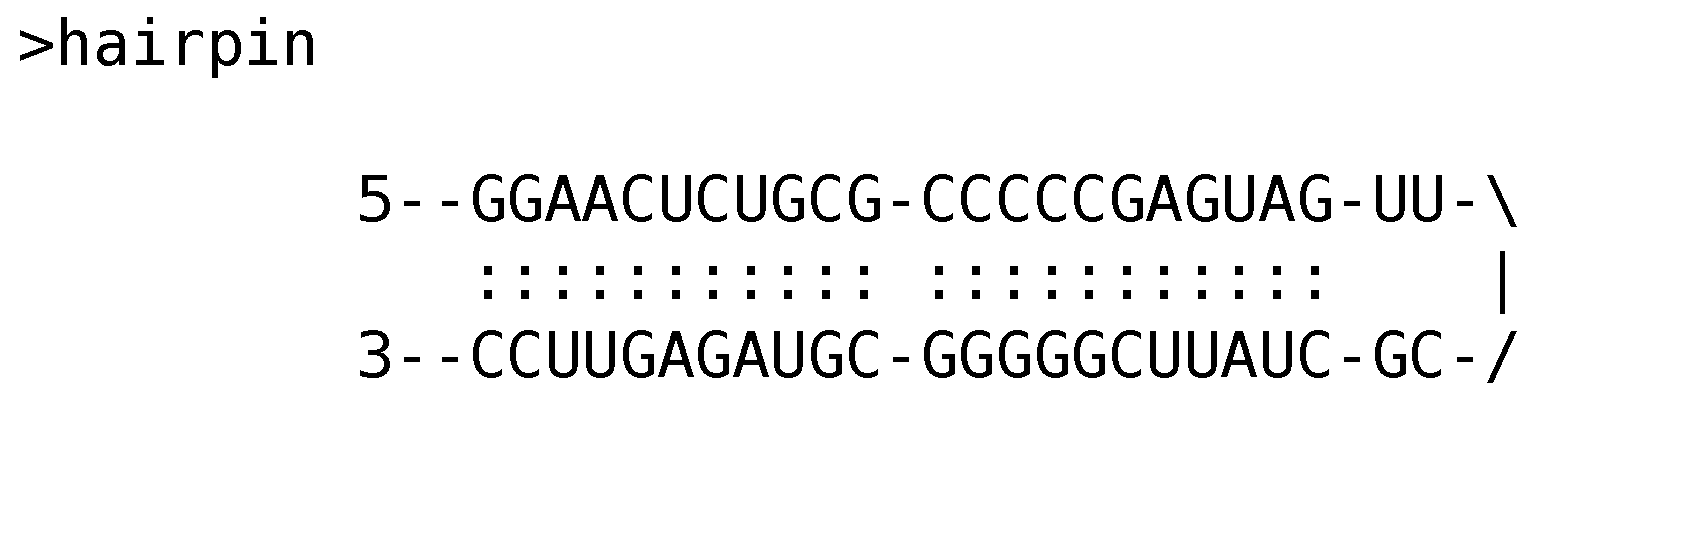
\includegraphics[align=c,width=\textwidth/3]{figures/oxrna_sims/hairpin.eps} \centering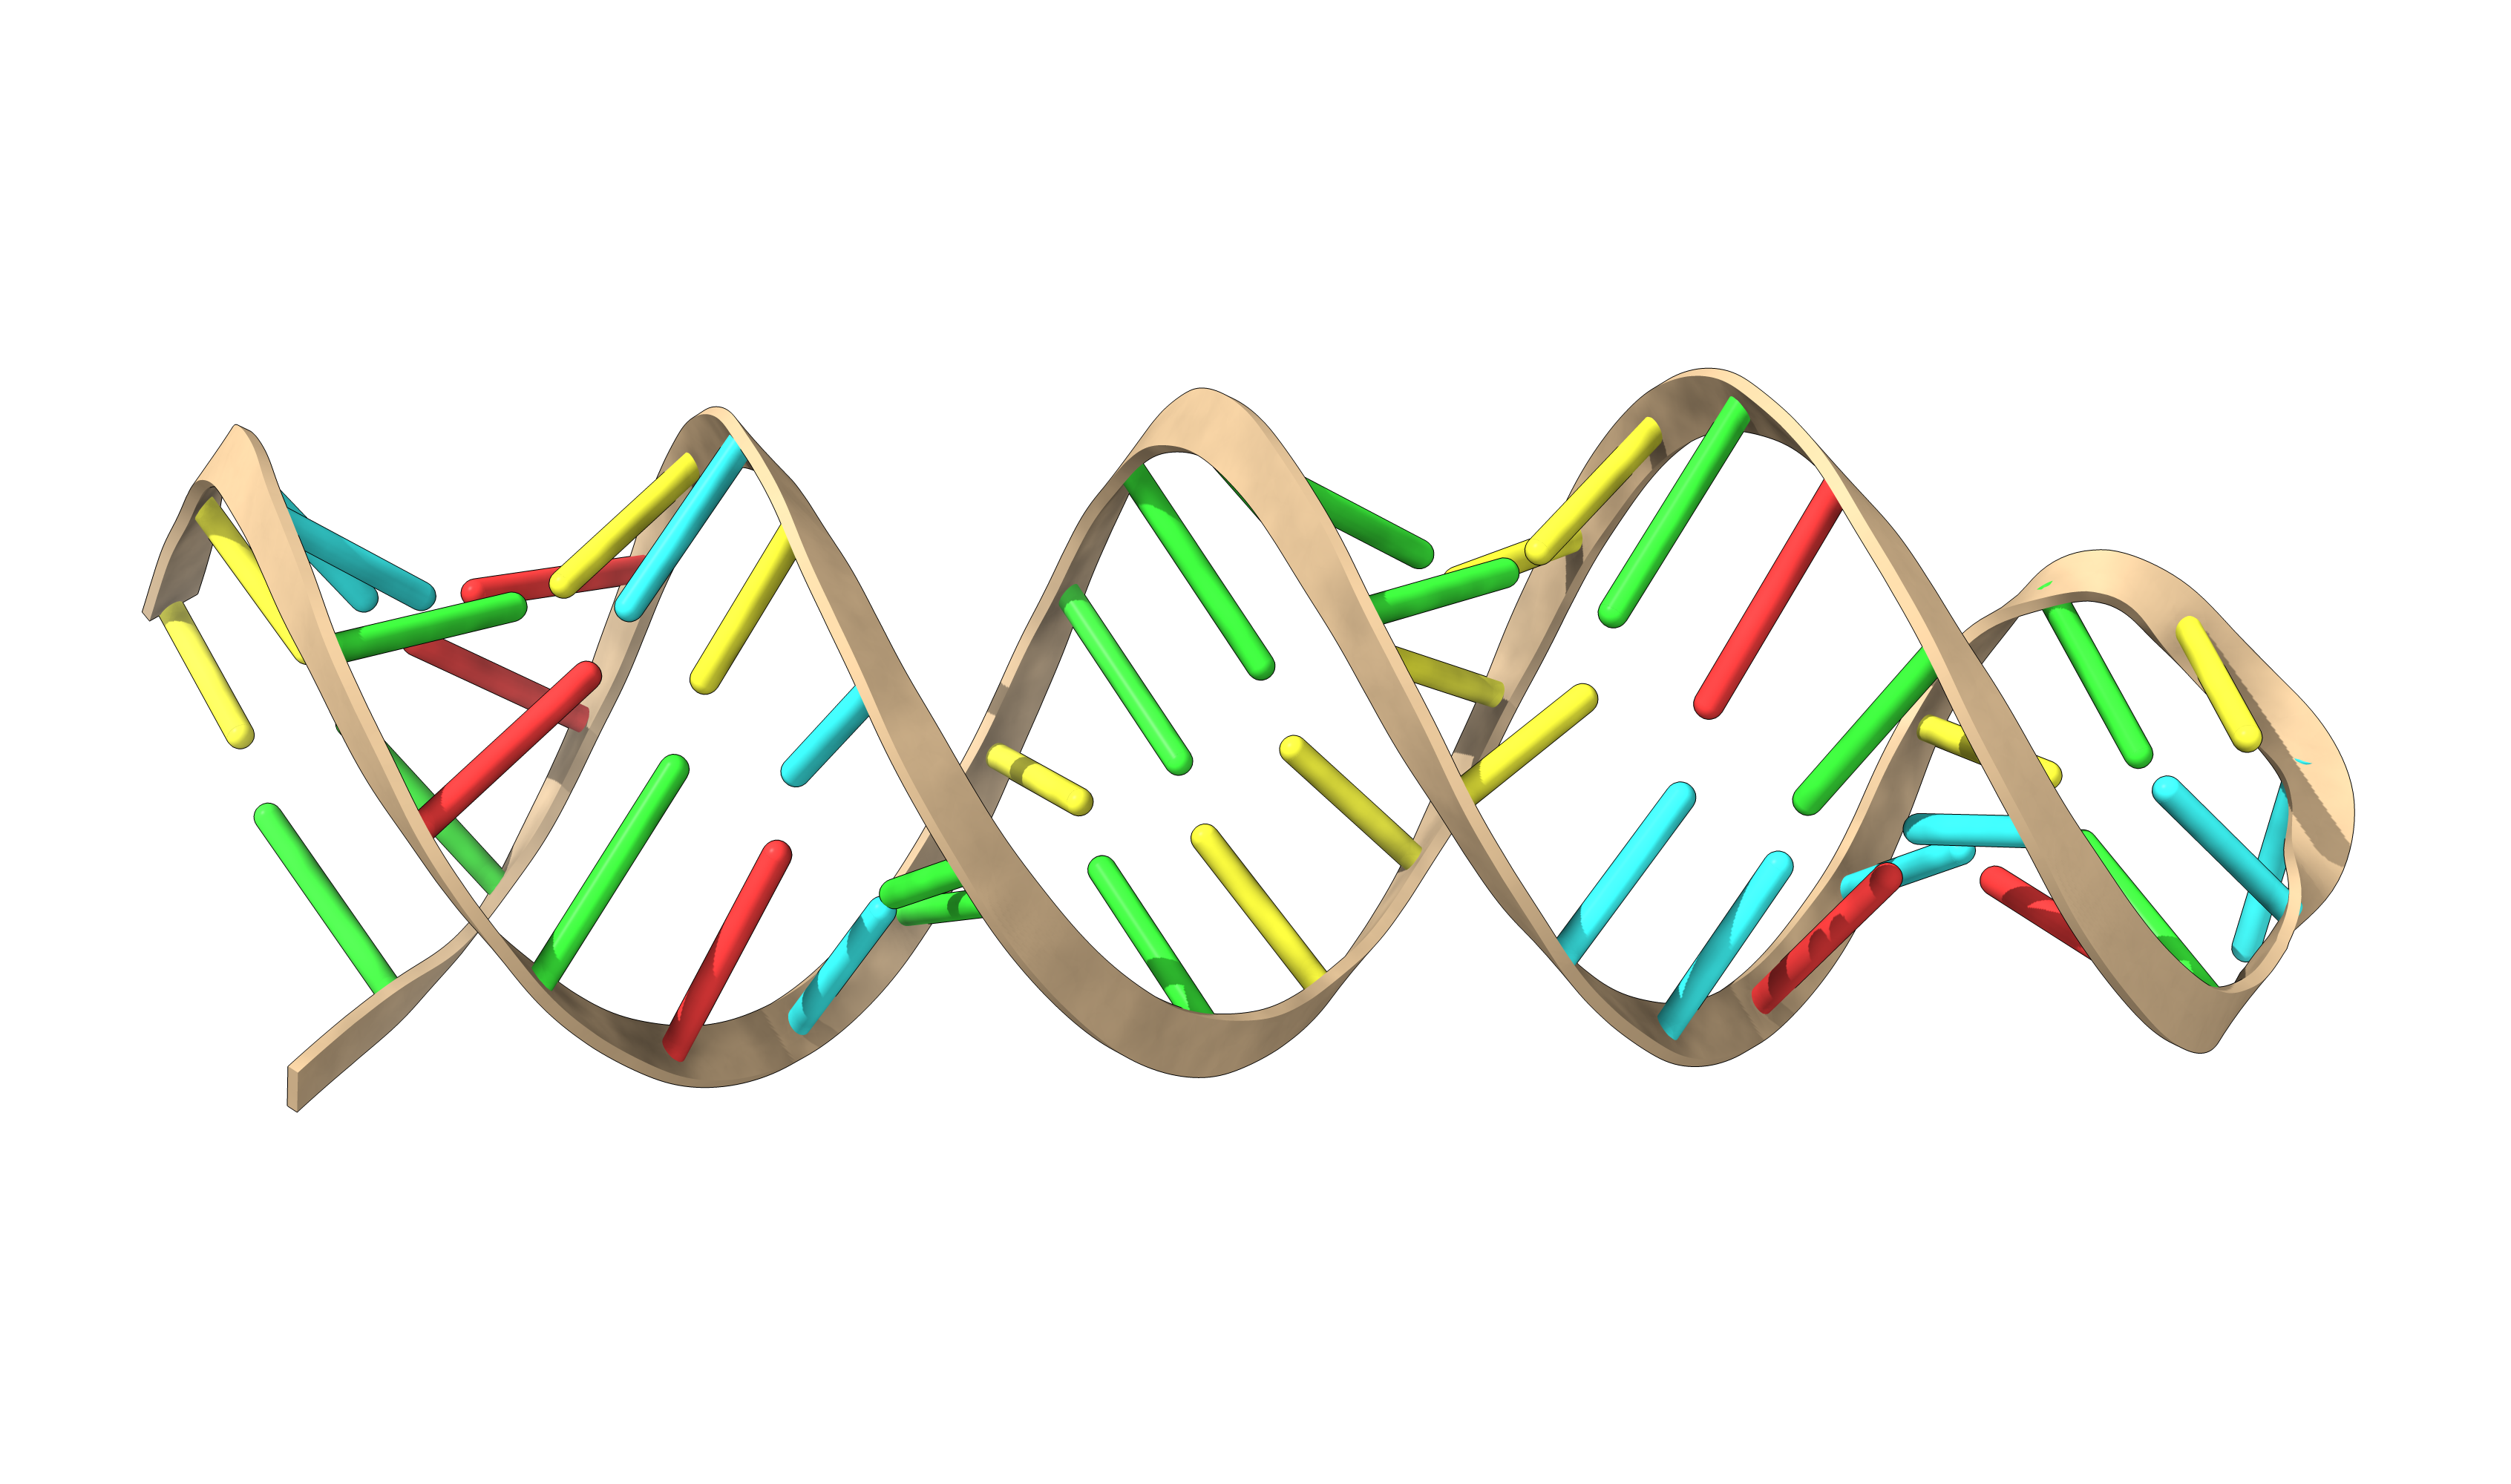
\includegraphics[align=c,width=\textwidth/3]{figures/oxrna_sims/hairpin.png} \centering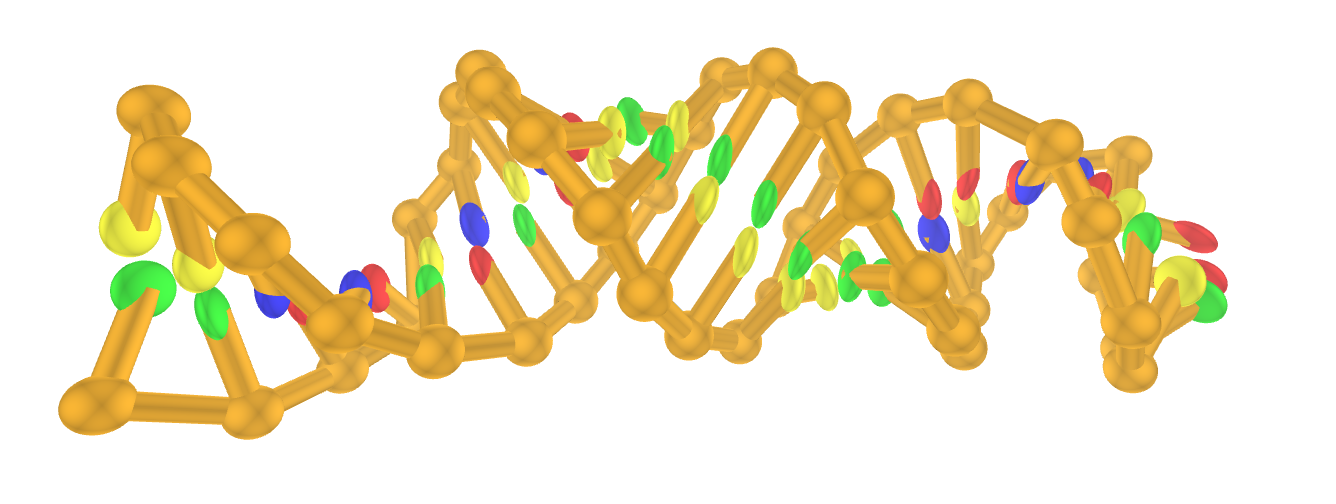
\includegraphics[align=c,width=\textwidth/3]{figures/oxrna_sims/hairpin_last_conf.png}
}
\makebox[\textwidth][c]{b)  
  \centering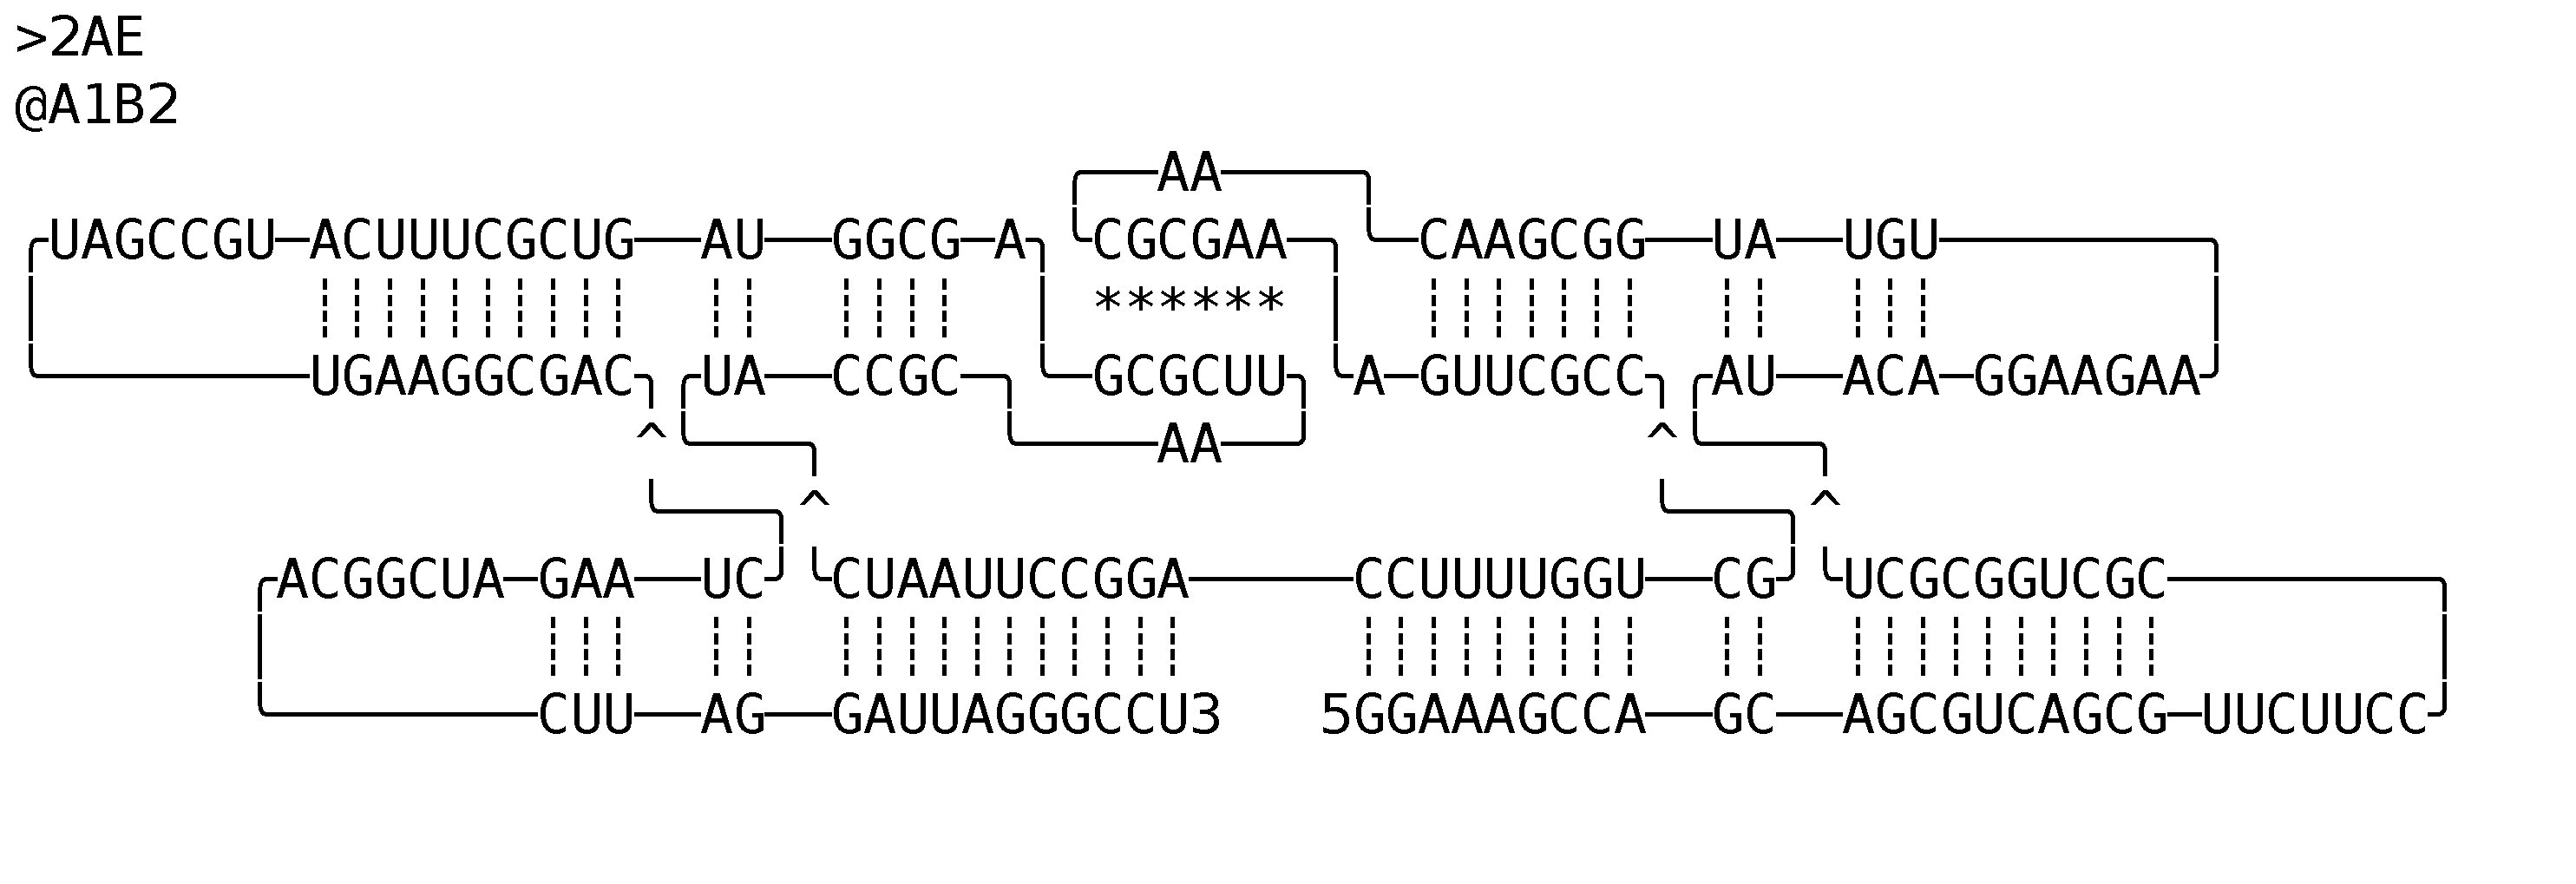
\includegraphics[align=c,width=\textwidth/3]{figures/oxrna_sims/2AE.eps} \centering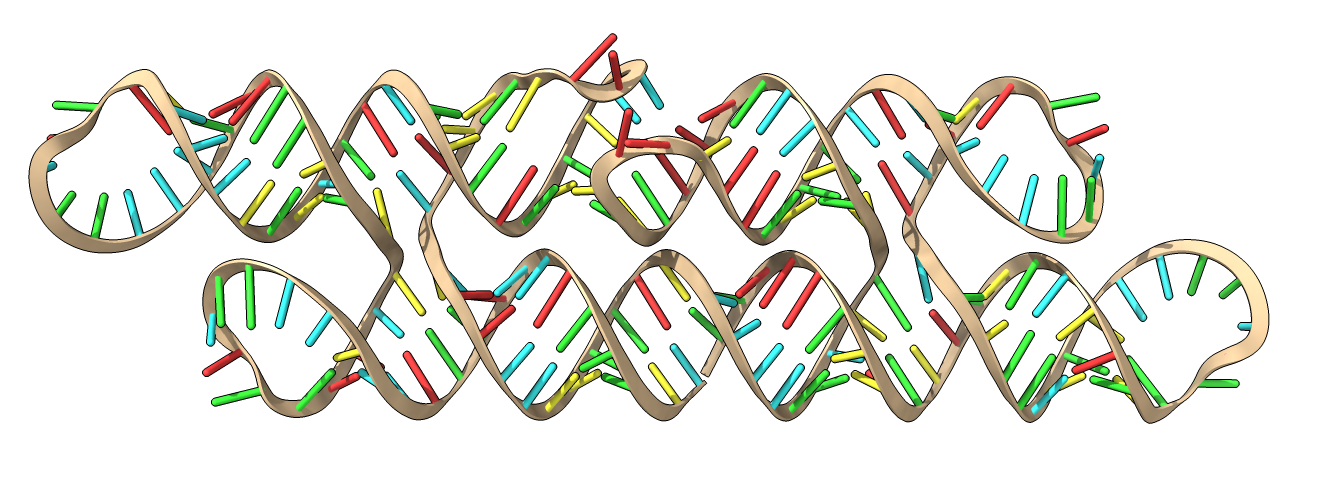
\includegraphics[align=c,width=\textwidth/3]{figures/oxrna_sims/2AE.png} \centering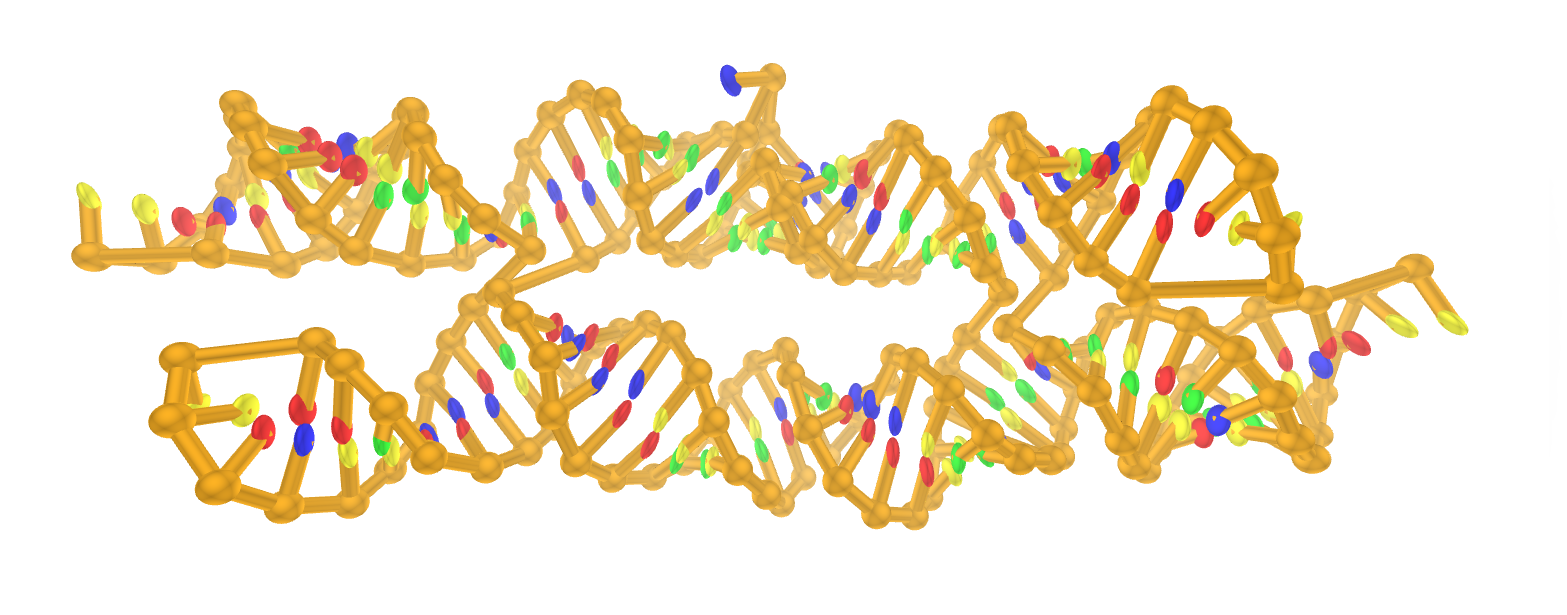
\includegraphics[align=c,width=\textwidth/3]{figures/oxrna_sims/2AE_last_conf.png}
}
\makebox[\textwidth][c]{c) 
  \centering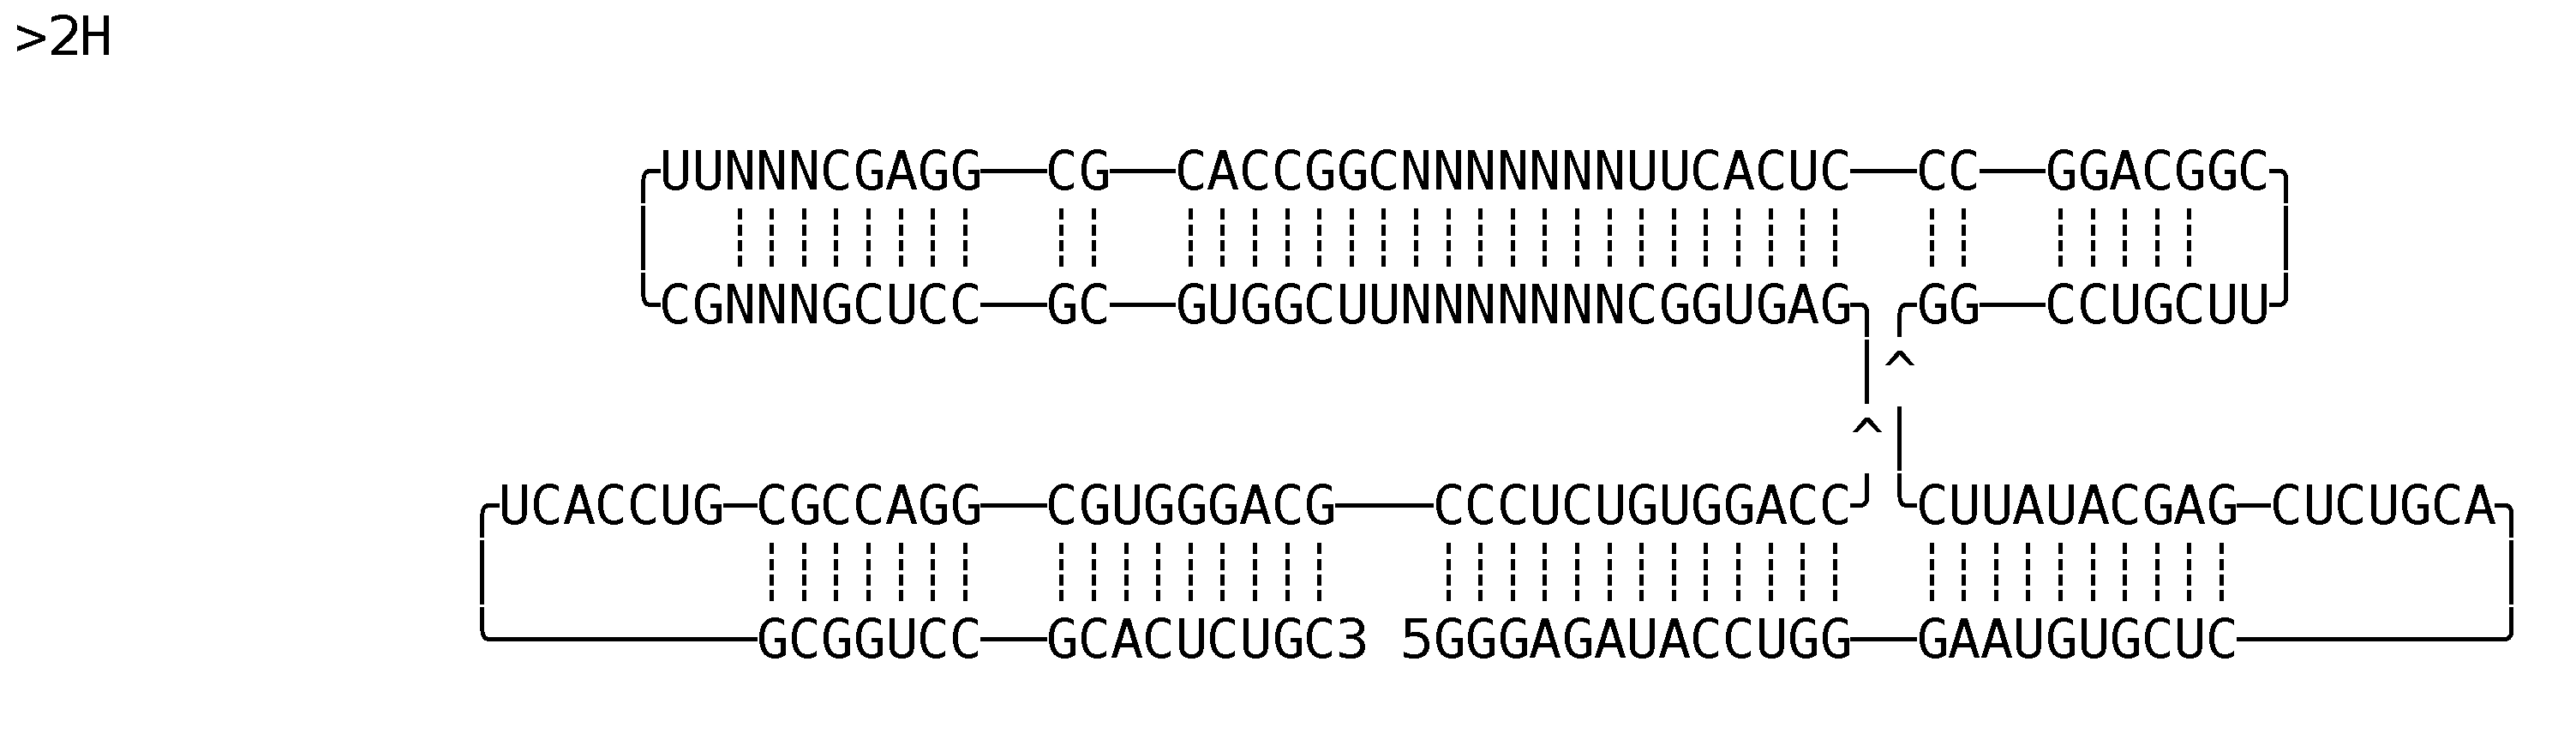
\includegraphics[align=c,width=\textwidth/3]{figures/oxrna_sims/2H.eps} \centering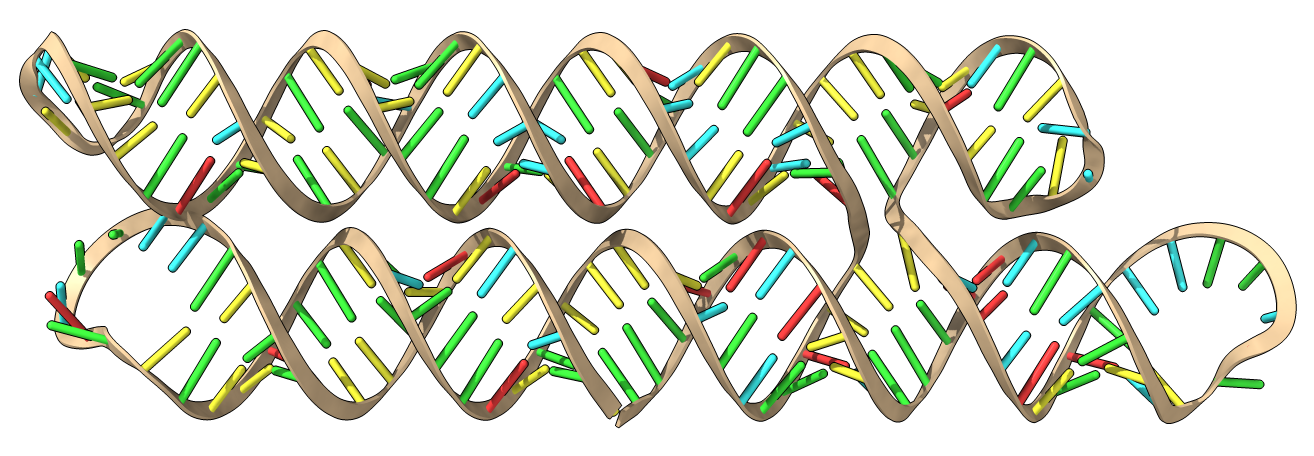
\includegraphics[align=c,width=\textwidth/3]{figures/oxrna_sims/2H.png}
  \centering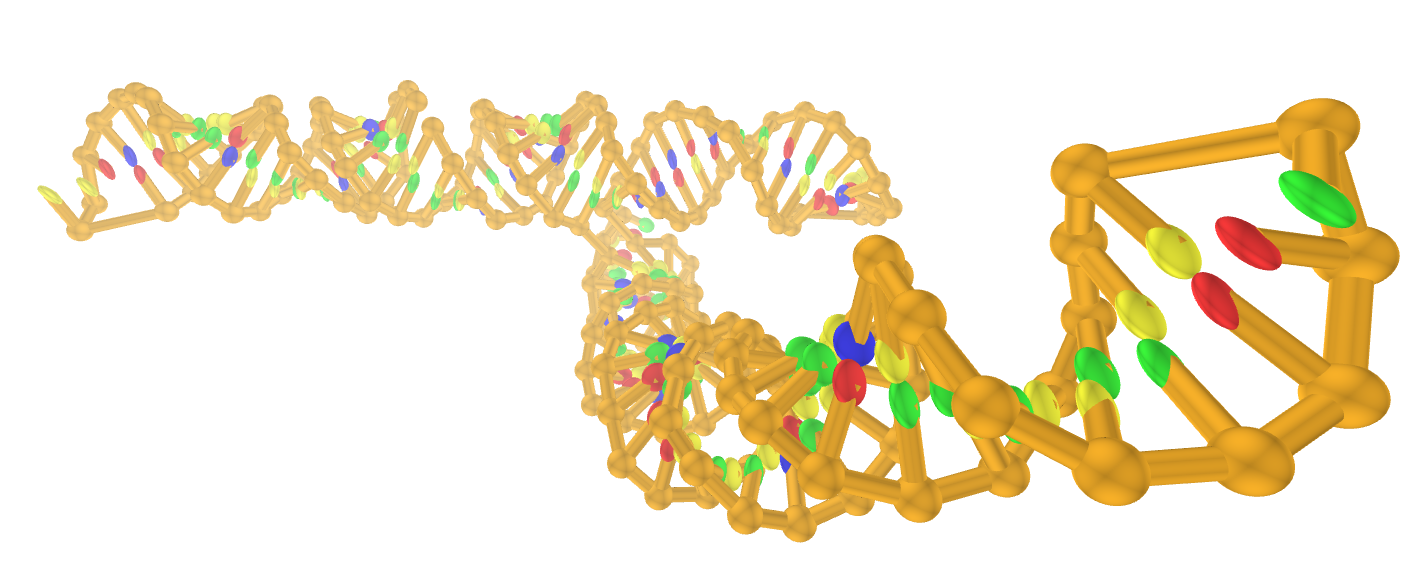
\includegraphics[align=c,width=\textwidth/3]{figures/oxrna_sims/2H_last_conf.png}
}
\makebox[\textwidth][c]{d) 
  \centering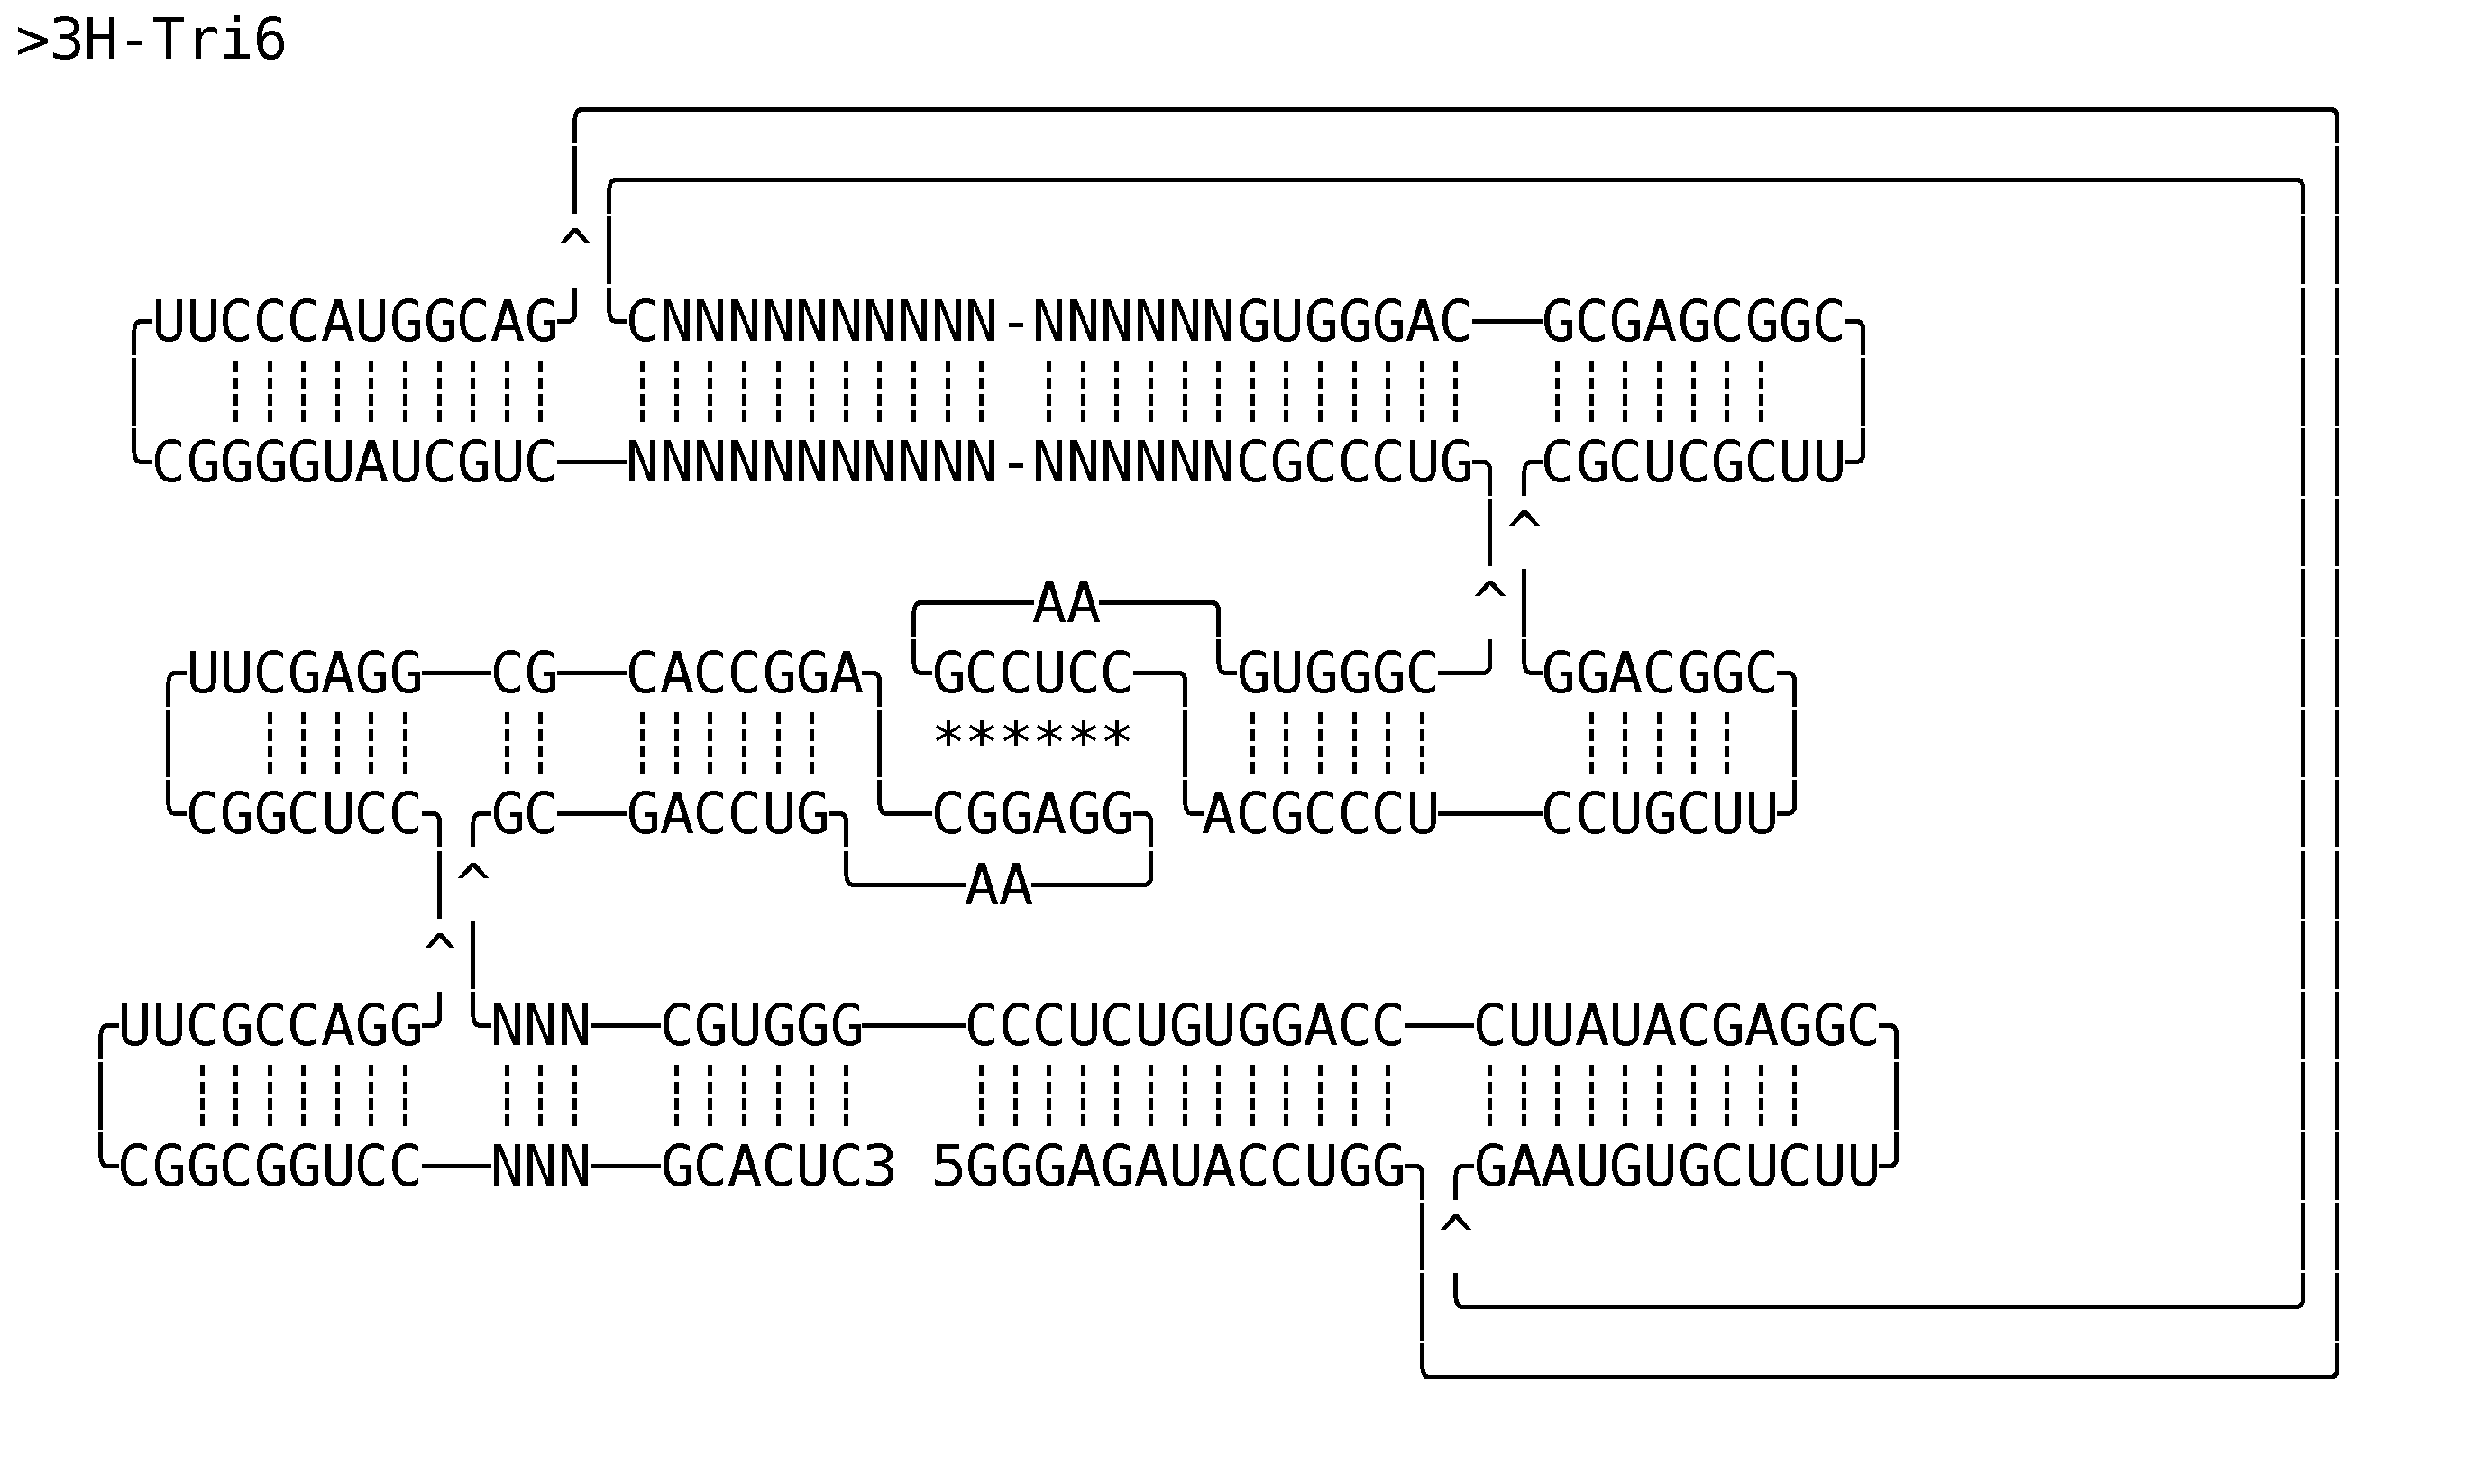
\includegraphics[align=c,width=\textwidth/3]{figures/oxrna_sims/3H-Tri6.eps} \centering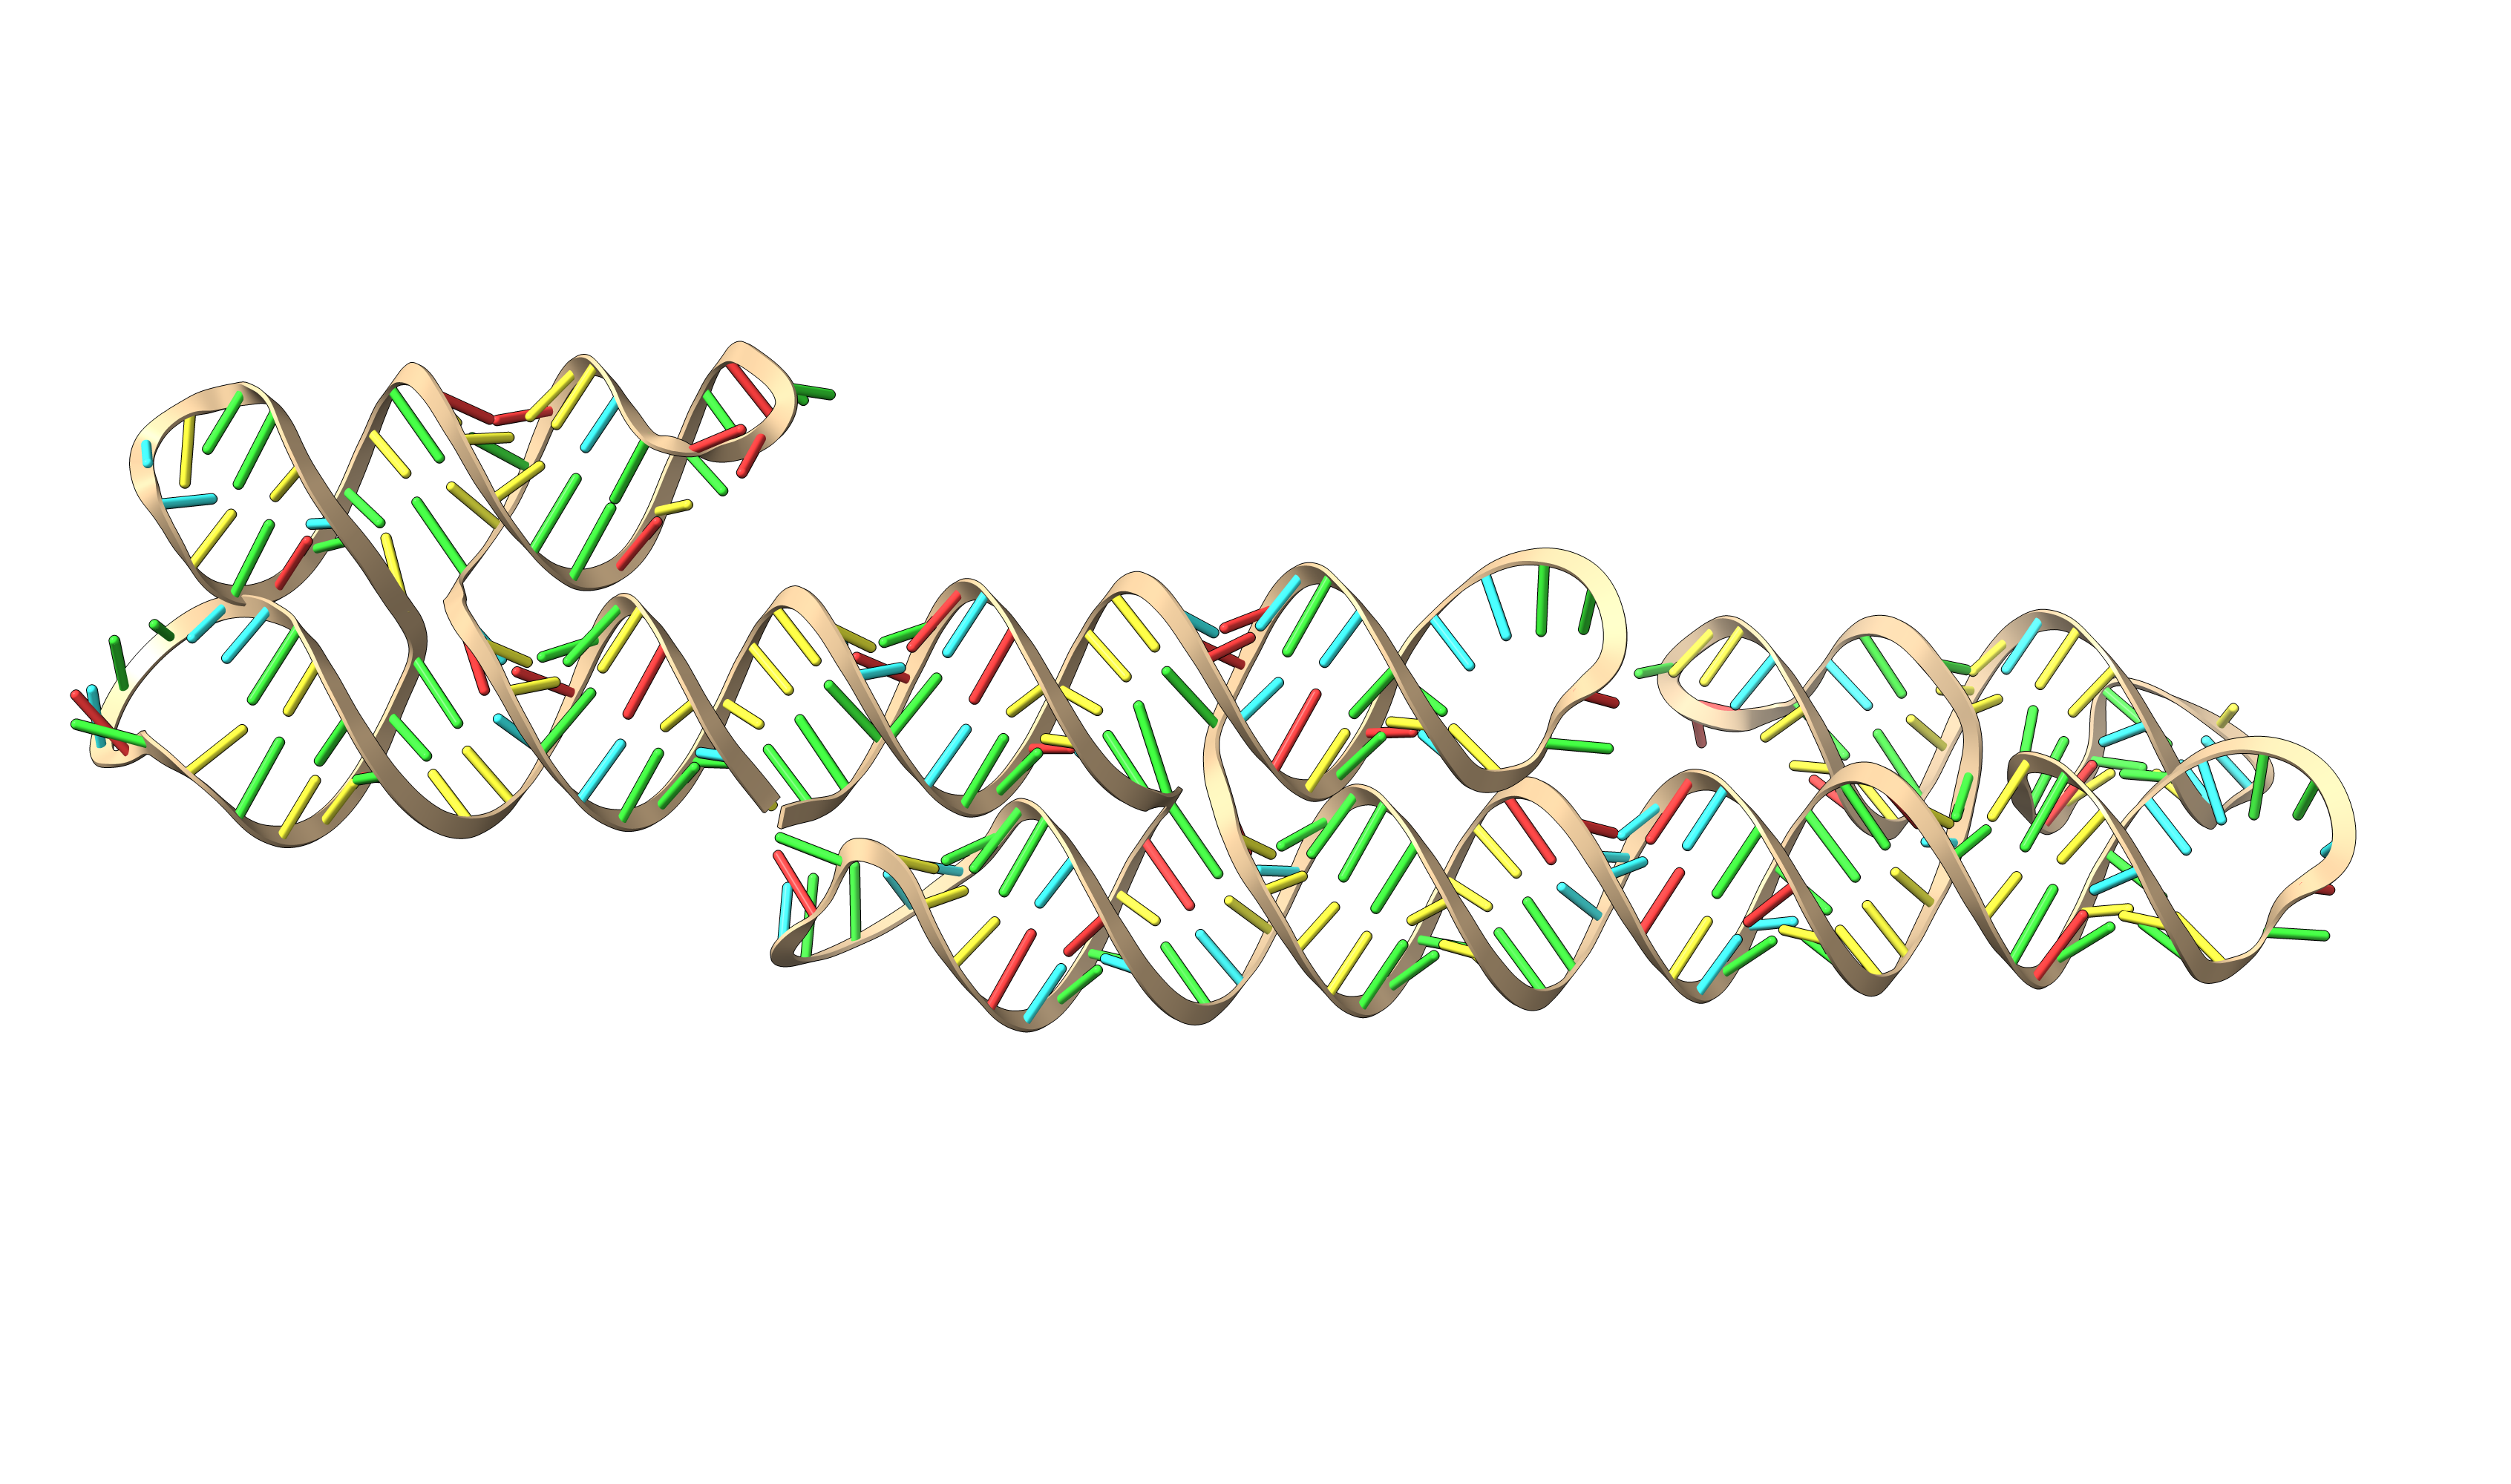
\includegraphics[align=c,width=\textwidth/3]{figures/oxrna_sims/3H-Tri6_pre.png}
  \centering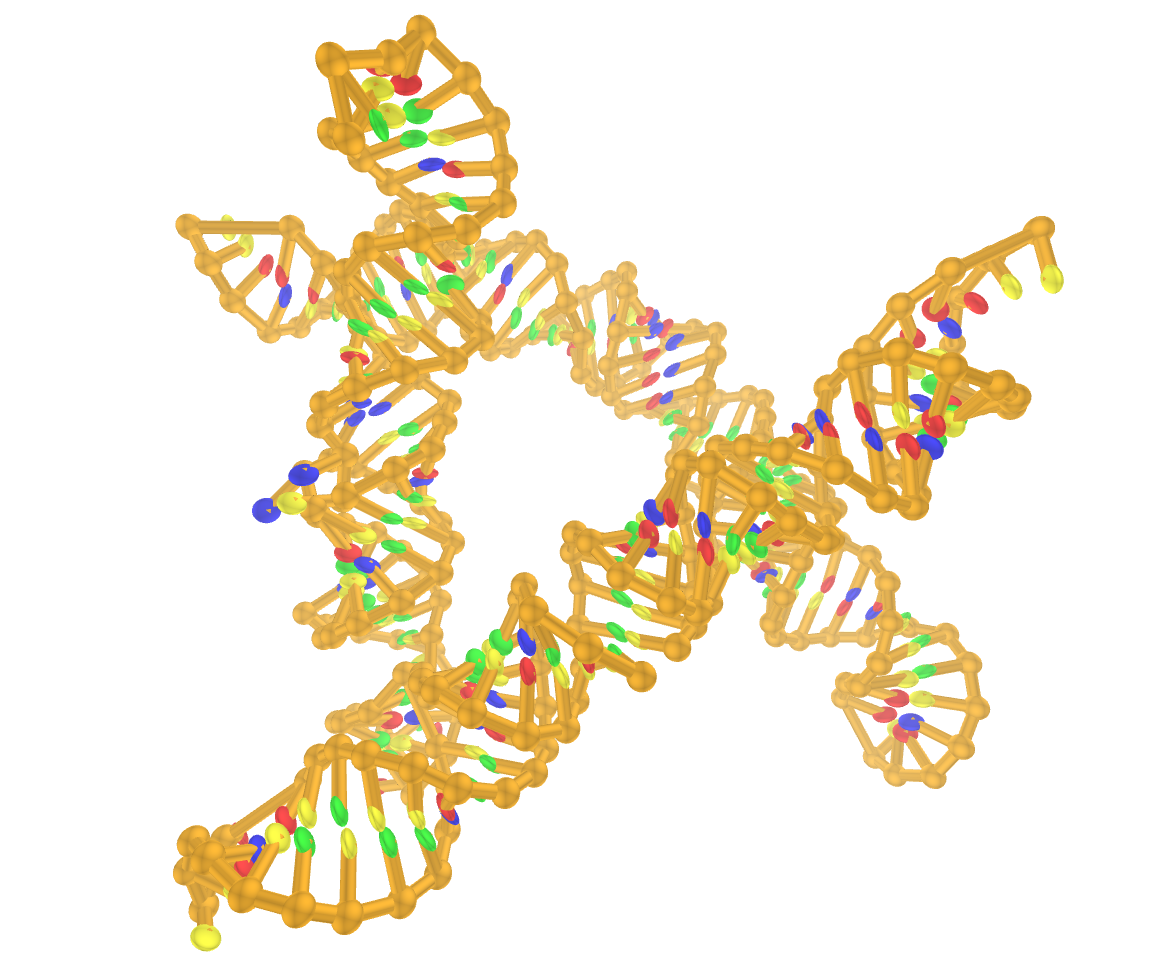
\includegraphics[align=c,width=\textwidth/3]{figures/oxrna_sims/2H-Tri6_tri.png}
}
\makebox[\textwidth][c]{e)  
  \centering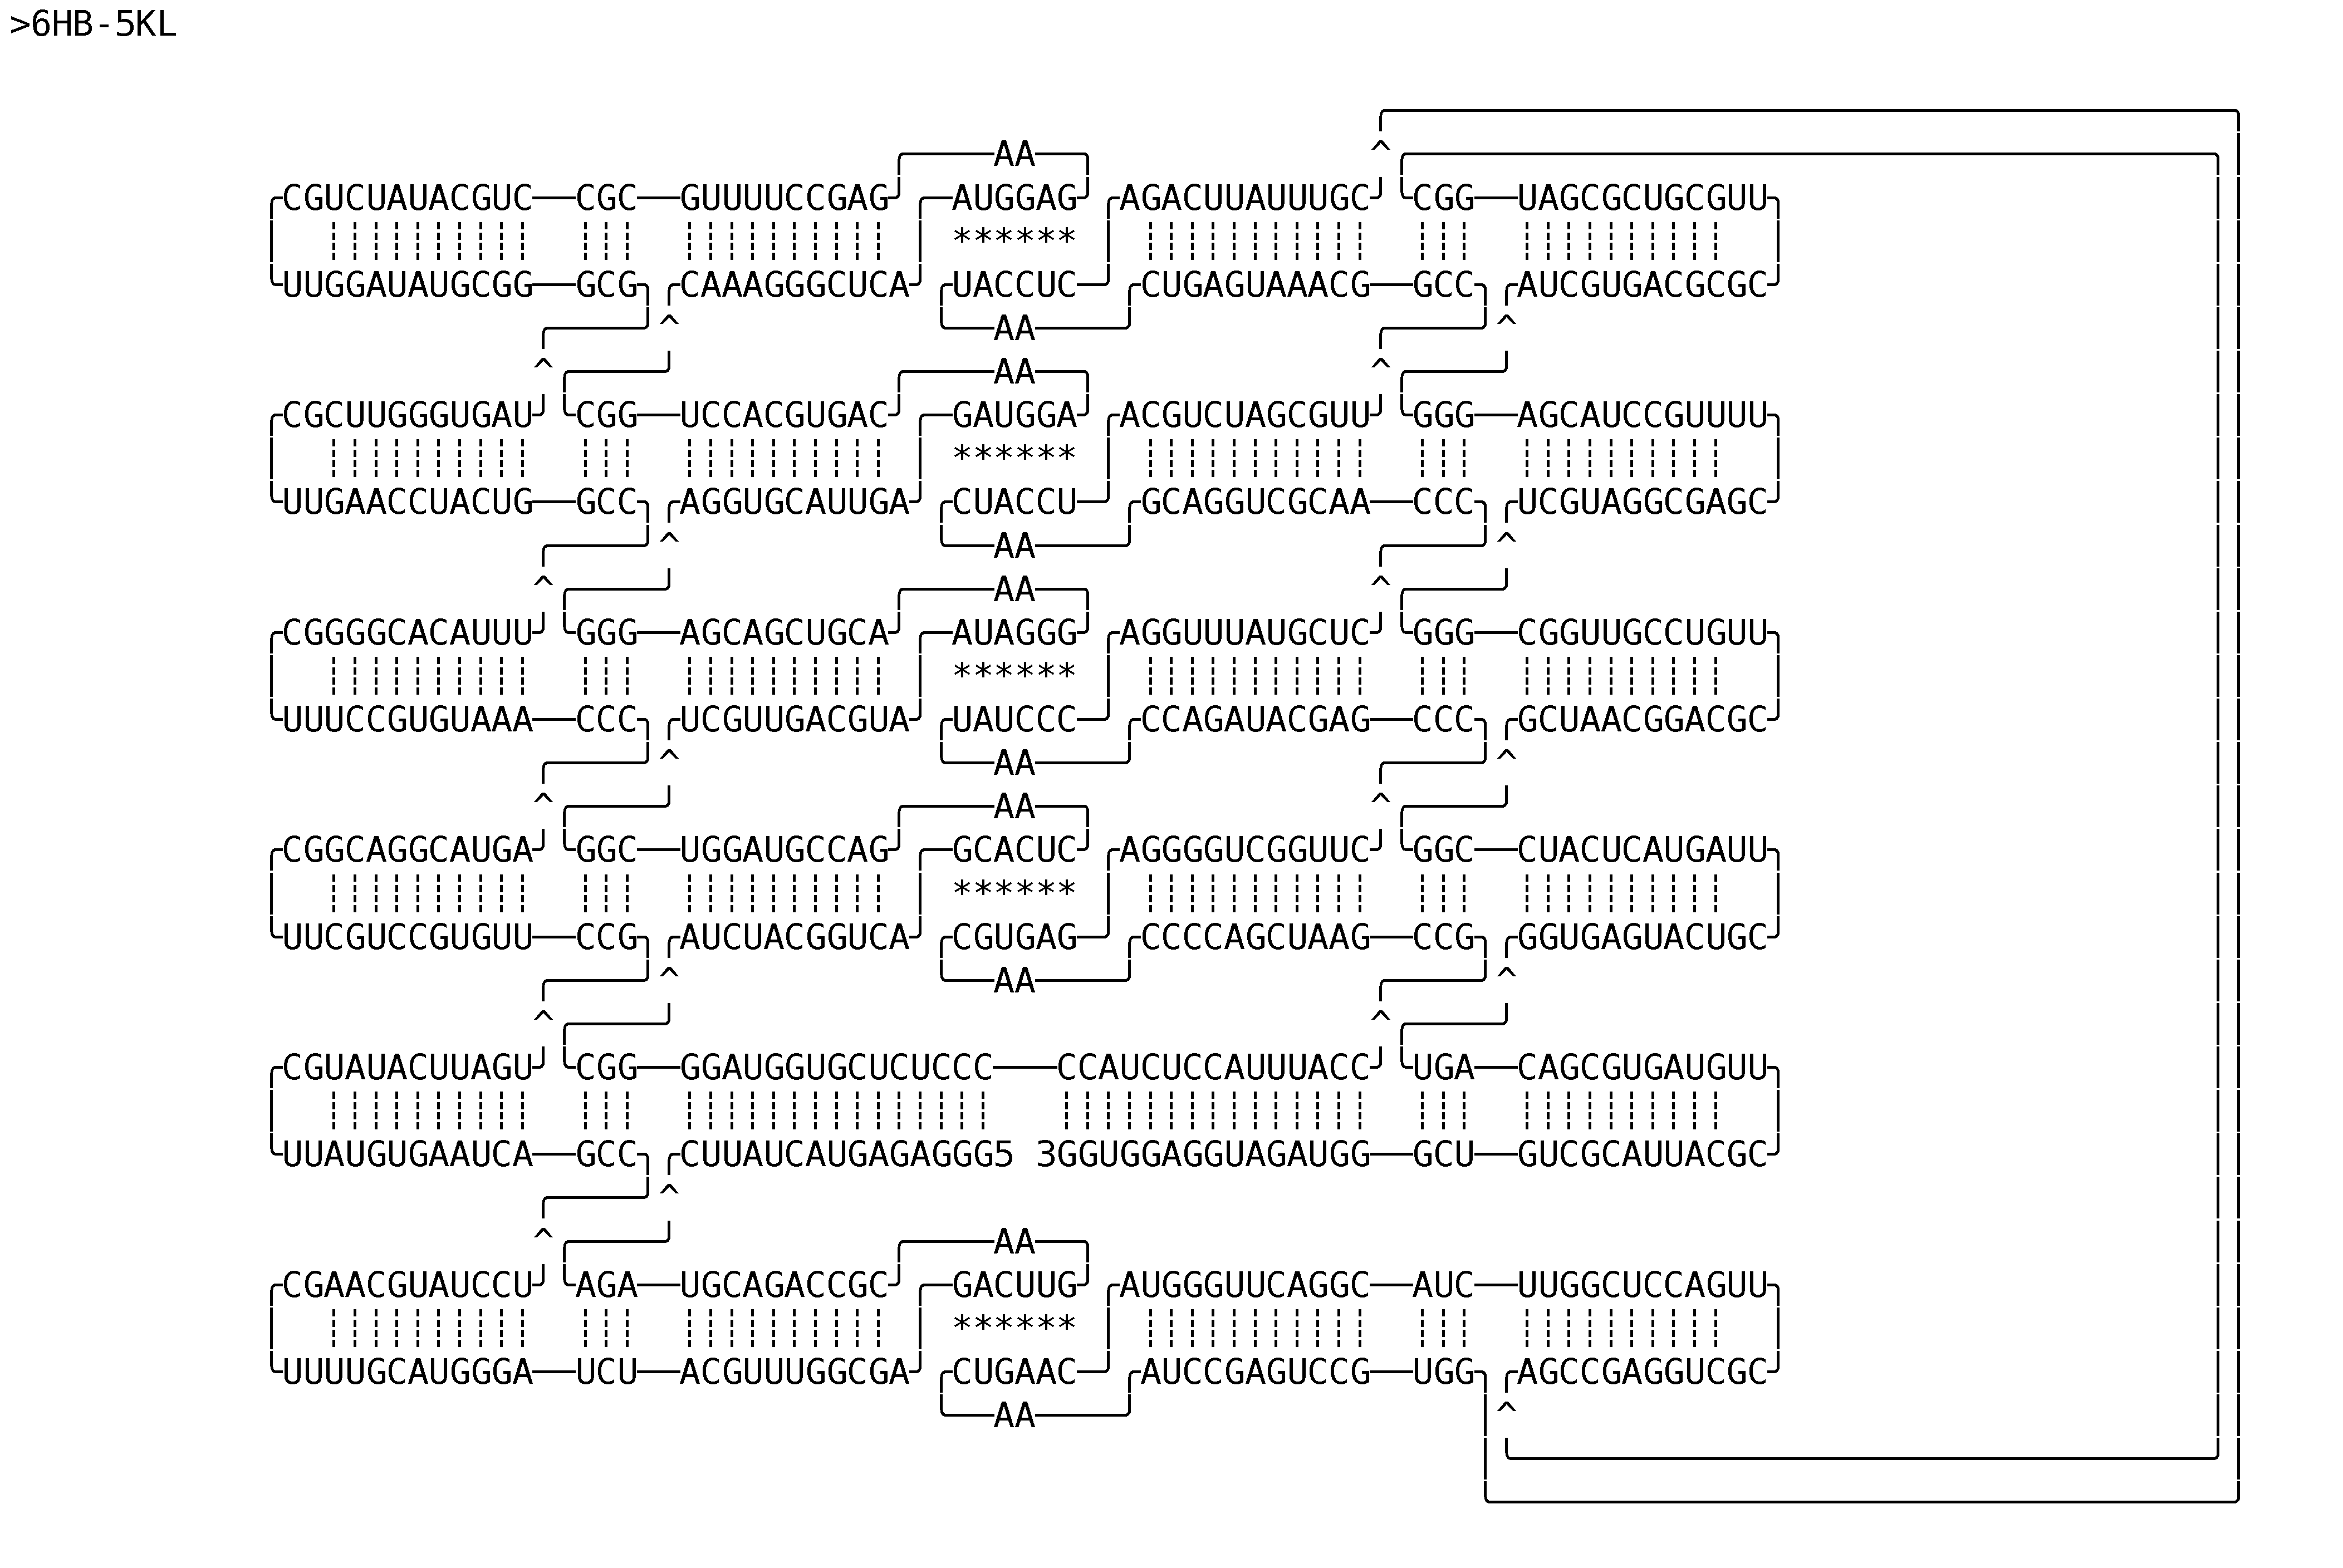
\includegraphics[align=c,width=\textwidth/3]{figures/oxrna_sims/6HB-5KL.eps} \centering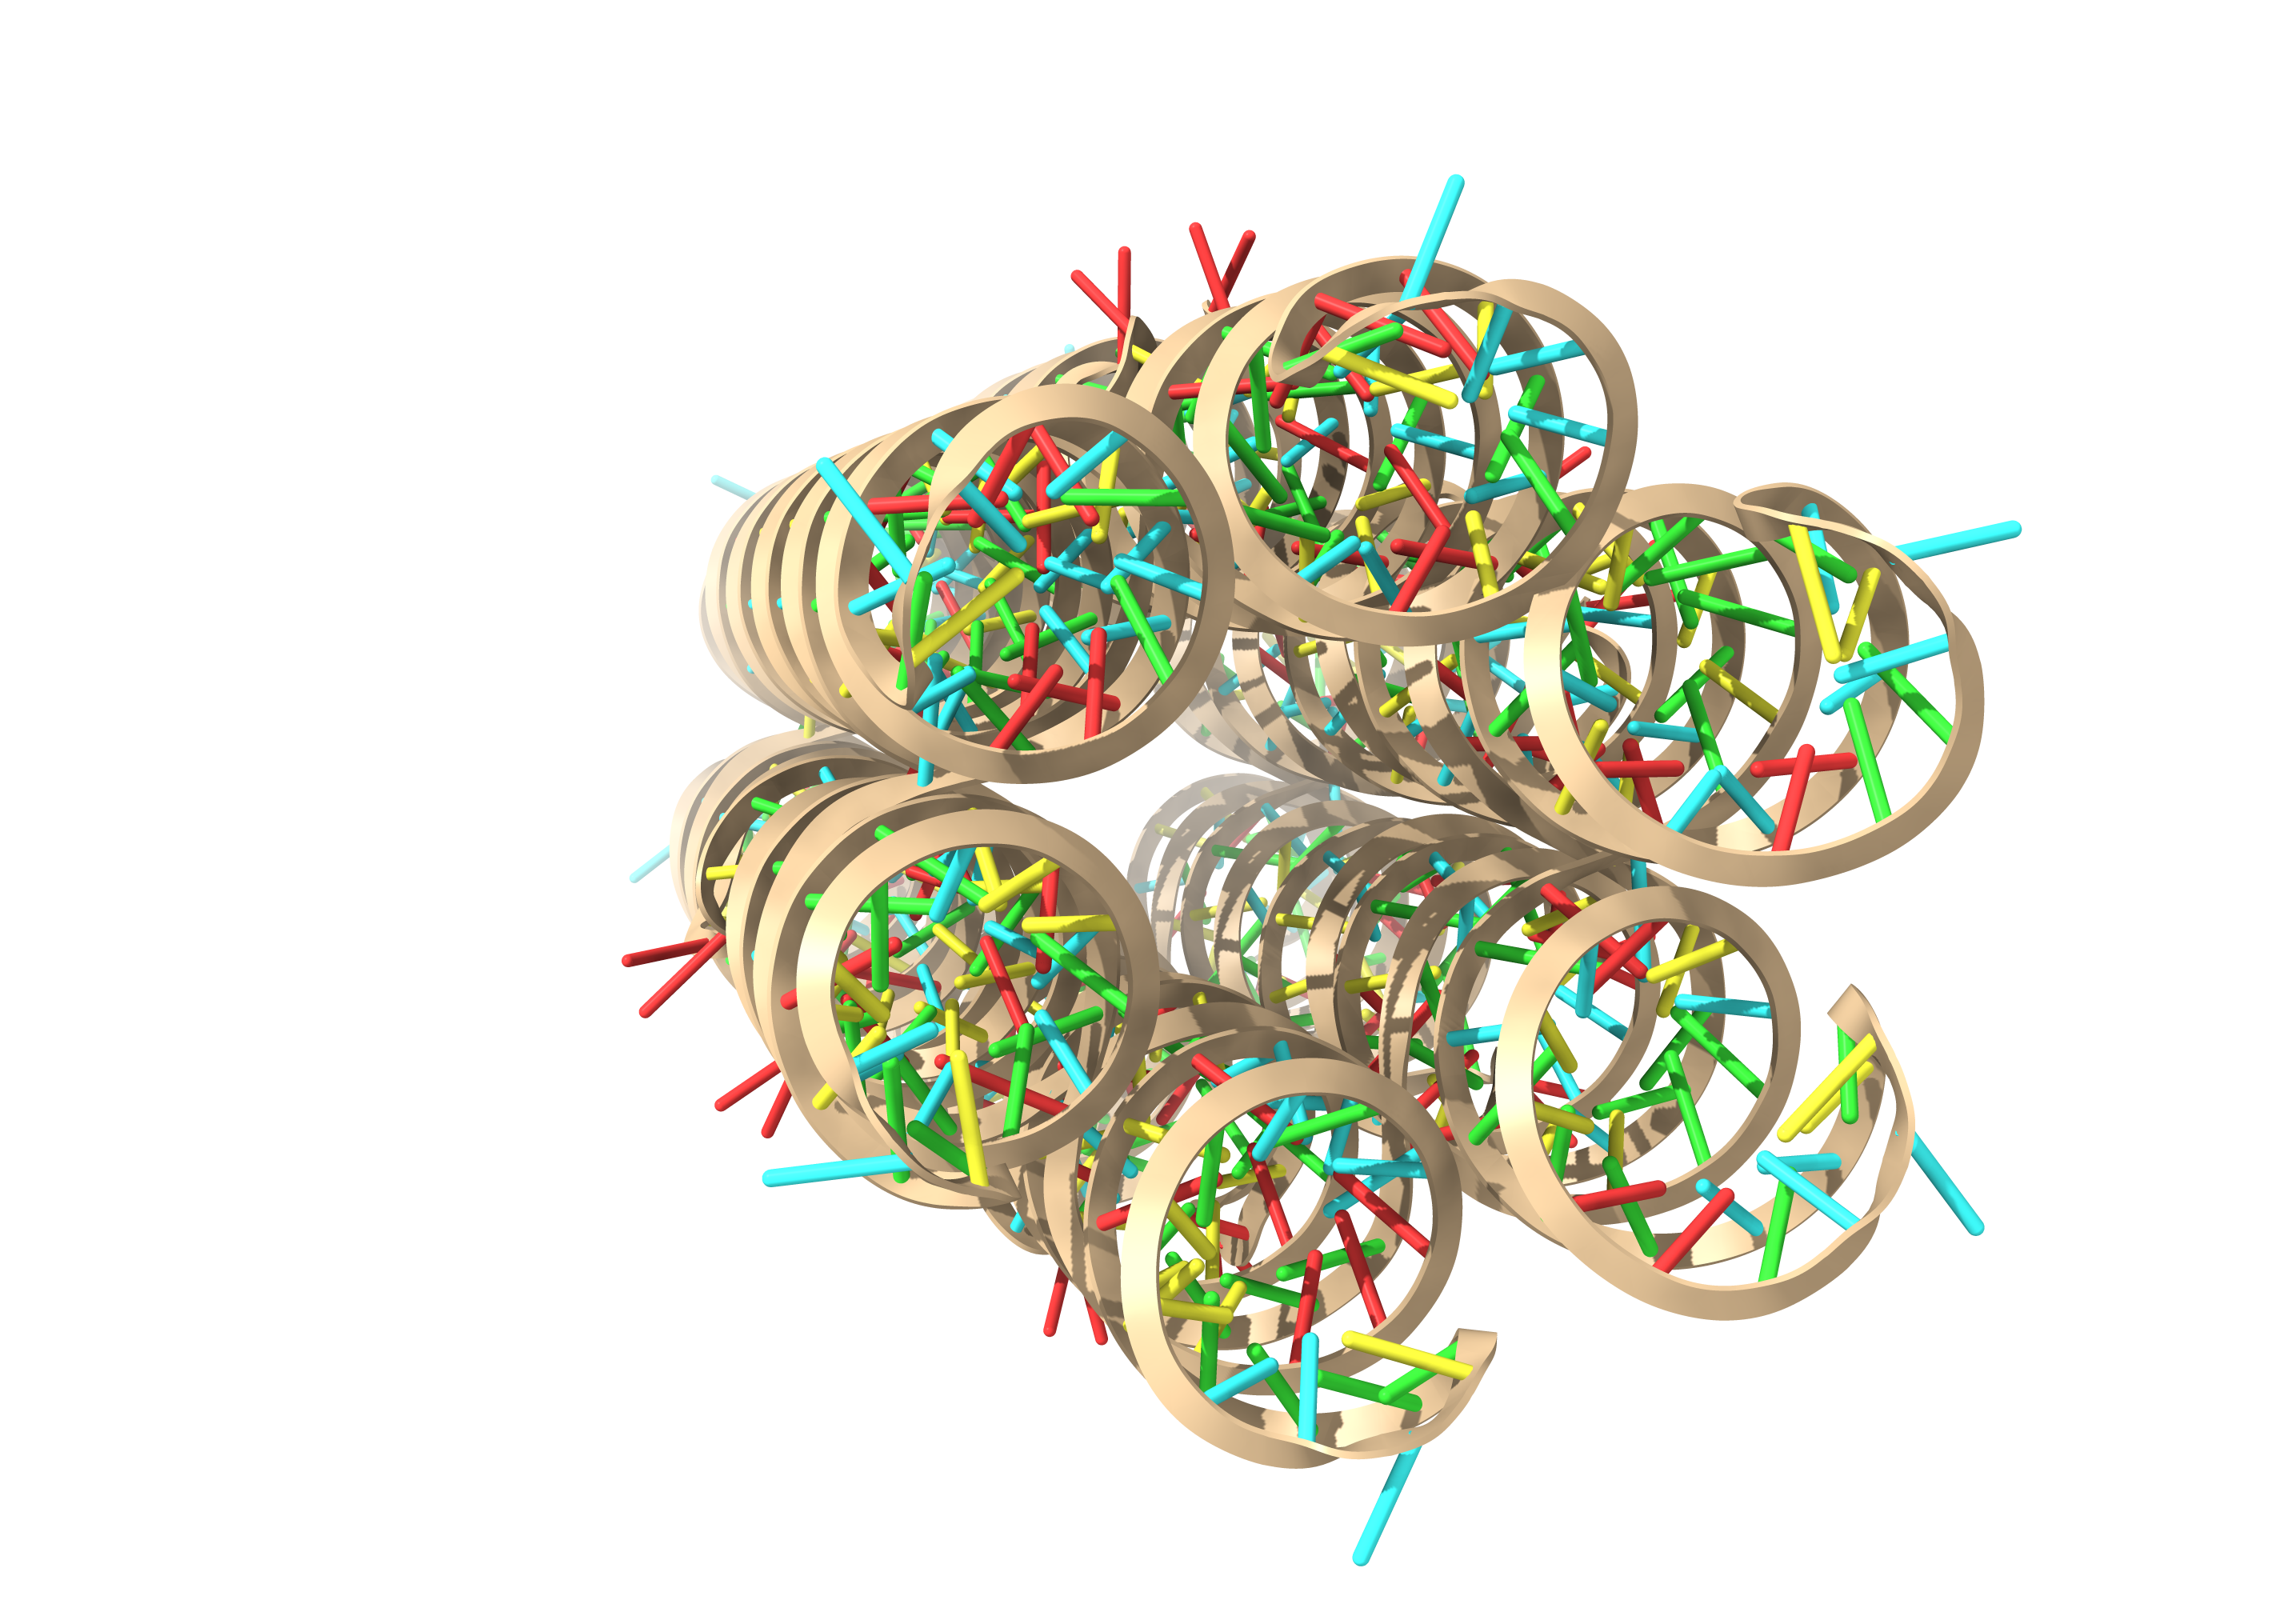
\includegraphics[align=c,width=\textwidth/3]{figures/oxrna_sims/6HB-5KL.png}
  \centering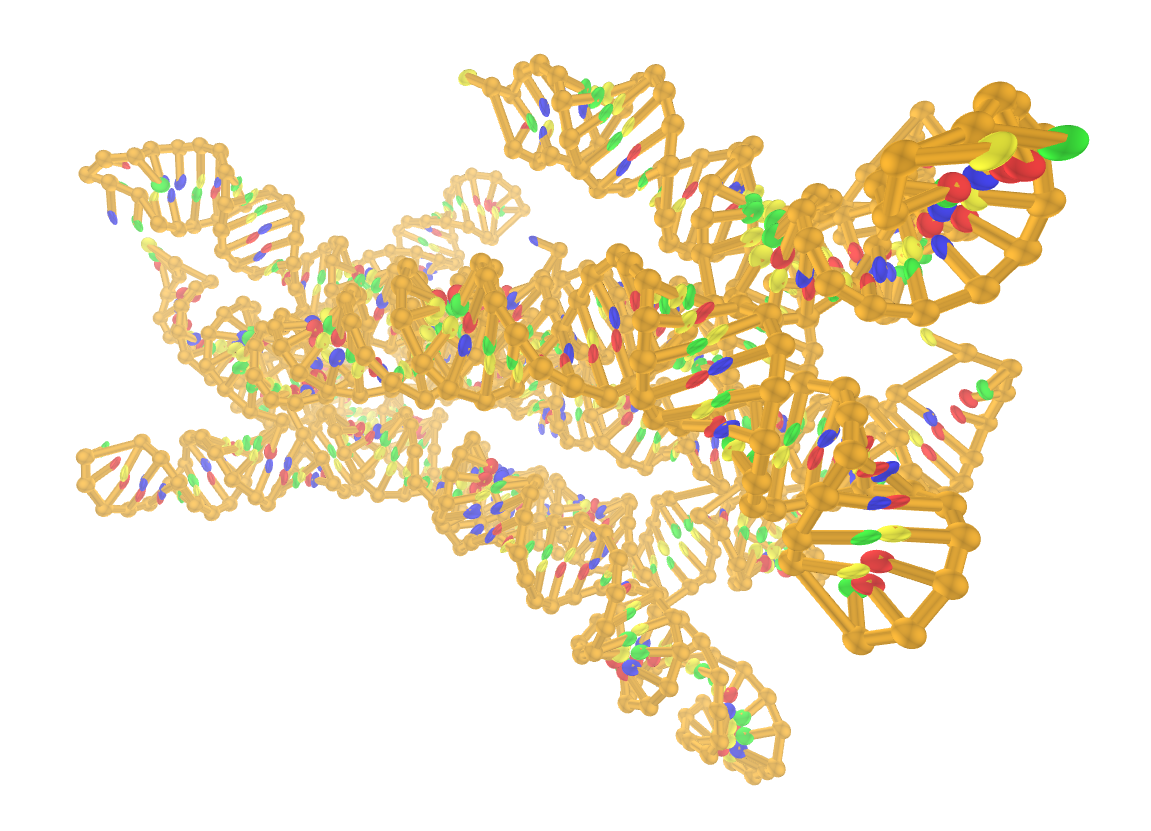
\includegraphics[align=c,width=\textwidth/3]{figures/oxrna_sims/6HB-5KL_last_conf.png}
}
\end{center}
\caption{Conversion and simulation of various RNA designs. Each row, from left to right, shows the ASCII blueprint design, the PDB model (visualised using ChimeraX), and a frame from the simulated structure (visualised using oxView).  \textbf{a)} Is a simple hairpin loop.  \textbf{b)} is a two-helix bundle tile used in \cite{geary2014single}.  \textbf{c)} is two helices connected by a double crossover, analysing the flexibility of such a motif.  \textbf{d)} is a possible design for a tensegrity triangle.  \textbf{e)} is a siz-helix bundle.}
\label{fig:oxRNA_sims}\end{figure}




\begin{savequote}[8cm]
You live and learn. At any rate, you live.
  \qauthor{--- Douglas Adams, Mostly Harmless}
\end{savequote}

\chapter{Conclusion}

In conclusion, nanostructures self-assembly design has been investigated on both an abstract and a more detailed level. The presented projects have resulted in tools and methods for creating, simulating and analysing self-limiting modular structures with minimal complexity, potentially containing building blocks created in different design software.

\section{Individual module design}

\section{Modular assembly}

\section{Future work}

Staged assembly

Given a maximum complexity - for example, a limited number of possible colours - what is the largest bounded structure that can deterministically assemble?


%% APPENDICES %% 
% Starts lettered appendices, adds a heading in table of contents, and adds a page that just says "Appendices" to signal the end of your main text.
\startappendices
% Add or remove any appendices you'd like here:
\begin{savequote}[8cm]
\textlatin{Cor animalium, fundamentum e\longs t vitæ, princeps omnium, Microco\longs mi Sol, a quo omnis vegetatio dependet, vigor omnis \& robur emanat.}

The heart of animals is the foundation of their life, the sovereign of everything within them, the sun of their microcosm, that upon which all growth depends, from which all power proceeds.
  \qauthor{--- William Harvey \cite{harvey_exercitatio_1628}}
\end{savequote}

\chapter{Possible appendix chapter}

\minitoc

Appendices are just like chapters.  Their sections and subsections get numbered and included in the table of contents; figures and equations and tables added up, etc.  Lorem ipsum dolor sit amet, consectetur adipiscing elit. Sed et dui sem. Aliquam dictum et ante ut semper. Donec sollicitudin sed quam at aliquet. Sed maximus diam elementum justo auctor, eget volutpat elit eleifend. Curabitur hendrerit ligula in erat feugiat, at rutrum risus suscipit. Pellentesque habitant morbi tristique senectus et netus et malesuada fames ac turpis egestas. Integer risus nulla, facilisis eget lacinia a, pretium mattis metus. Vestibulum aliquam varius ligula nec consectetur. Maecenas ac ipsum odio. Cras ac elit consequat, eleifend ipsum sodales, euismod nunc. Nam vitae tempor enim, sit amet eleifend nisi. Etiam at erat vel neque consequat.


%%%%% REFERENCES

% JEM: Quote for the top of references (just like a chapter quote if you're using them).  Comment to skip.
%\begin{savequote}[8cm]
%The first kind of intellectual and artistic personality belongs to the hedgehogs, the second to the foxes \dots
%  \qauthor{--- Sir Isaiah Berlin \cite{berlin_hedgehog_2013}}
%\end{savequote}

\setlength{\baselineskip}{0pt} % JEM: Single-space References

{\renewcommand*\MakeUppercase[1]{#1}%
\printbibliography[heading=bibintoc,title={\bibtitle}]}


\end{document}
